\documentclass[letterpaper,titlepage,12pt,oneside,spanish,final]{report_eie}

%\documentclass[letterpaper,titlepage,12pt,twoside,openright,spanish,final]{report_eie}

%%%%%%%%%%%%%%%%%%%%%%%%%%%%%%%%%%%%%%%%%%%%%%%%%%%%%%%%%%%%%%%%%%%%%%%%
\usepackage[spanish]{babel}
\usepackage[utf8]{inputenc}
\usepackage[T1]{fontenc}  %Estilo de fuente time new roman
\usepackage{amssymb}
\usepackage{amsfonts}
\usepackage{amsmath}
\usepackage{latexsym}
\usepackage[letterpaper]{geometry}

\usepackage{float}
\usepackage{makeidx}
\usepackage{color}
\usepackage{tocbibind}
\usepackage{acronym}
\usepackage{epsfig}
\usepackage{graphicx}
\usepackage{setspace}
\usepackage{multicol}
\usepackage{longtable}
%\usepackage{doublespace}
\usepackage[document]{ragged2e}
\usepackage{fancyhdr}
%\usepackage{fancyheadings}
\usepackage{indentfirst}
\usepackage{booktabs}
\usepackage{minted} % Formato de codigo en python
\usepackage{listings}
\usepackage{caption}
\usepackage{subcaption}
%========= Define el estilo de referencias ===============
%\usepackage[round,authoryear]{natbib}%\usepackage[square,numbers]{natbib}%
%\usepackage[comma,authoryear]{natbib} esto está abajo

%========= Define el estilo de referencias APA ===============
\usepackage[
backend=biber,
style=ieee,
citestyle=numeric
]{biblatex}

\addbibresource{referencias.bib} %Imports bibliography file
\usepackage{csquotes}
\usepackage[compact]{titlesec} %modificar espaciado


\usepackage{url}
\usepackage{hyperref}
%\usepackage[dvips,colorlinks=true,urlcolor=red,citecolor=black,anchorcolor=black,linkcolor=black]{hyperref}
%%%%%%%%%%%%%%%%%%%%%%%%%%%%%%%%%%%%%%%%%%%%%%%%%%%%%%%%%%%%%%%%%%
%            Definición del Documento PDF, (PDFLaTeX)            %
%%%%%%%%%%%%%%%%%%%%%%%%%%%%%%%%%%%%%%%%%%%%%%%%%%%%%%%%%%%%%%%%%%

\hypersetup{pdfauthor=Guillermo Raven}

\hypersetup{pdftitle=Trabajo Especial de Grado}%

\hypersetup{pdfkeywords=Robot manipulador}

\pdfstringdef{\Produce}{Escuela de Ingeniería Eléctrica, Facultad de Ingeniería, UCV}%

\pdfstringdef{\area}{Área del trabajo}

\hypersetup{pdfproducer=\Produce}

\hypersetup{pdfsubject=\area}

\hypersetup{bookmarksnumbered=true}

%%%%%%%%%%%%%%%%%%%%%%%%%%%%%%%%%%%%%%%%%%%%%%%%%%%%%%%%%%%%%%%%%%
%\setcounter{MaxMatrixCols}{10}


%===================== Re-definición de Ambientes =================
\newtheorem{theorem}{Teorema}
\newtheorem{acknowledgement}[theorem]{Acknowledgement}
\newtheorem{algoritmo}[theorem]{Algorithm}
\newtheorem{supuestos}[theorem]{Supuestos}
\newtheorem{hipotesis}[theorem]{Hipótesis}
\newtheorem{axiom}[theorem]{Axiom}
\newtheorem{case}[theorem]{Case}
\newtheorem{claim}[theorem]{Claim}
\newtheorem{conclusion}[theorem]{Conclusión}
\newtheorem{condition}{Condición}
\newtheorem{conjecture}{Conjecture}
\newtheorem{corollary}{Corollary}
\newtheorem{criterion}{Criterion}
\newtheorem{definition}{Definición}  %{Definition}
\newtheorem{example}[theorem]{Ejemplo}%{Example}
\newtheorem{exercise}[theorem]{Exercise}
\newtheorem{lemma}{Lemma}
\newtheorem{notation}[theorem]{Notation}
\newtheorem{problem}{Problem}
\newtheorem{property}{Property}
\newtheorem{proposition}{Proposition}
\newtheorem{remark}[theorem]{Remark}
\newtheorem{solution}{Solution}
\newtheorem{summary}[theorem]{Summary}
\newenvironment{proof}[1][Proof]{\noindent\textbf{#1.} }{\ \rule{0.5em}{0.5em}}%

\numberwithin{equation}{chapter}%
\numberwithin{figure}{chapter}%
\numberwithin{table}{chapter}%
\numberwithin{definition}{chapter}%
\numberwithin{lemma}{chapter}%
\numberwithin{theorem}{chapter}%
\numberwithin{corollary}{chapter}%
\numberwithin{condition}{chapter}%
\numberwithin{criterion}{chapter}%
 \numberwithin{problem}{chapter}%
\numberwithin{property}{chapter}%
\numberwithin{proposition}{chapter}%
\numberwithin{solution}{chapter}%
\numberwithin{conjecture}{chapter}%

%==================== Separación en sílabas ========================
\hyphenpenalty=6800%

%A
\hyphenation{a-pro-xi-ma-do}


%B
\hyphenation{ba-lan-ce}%

%C
\hyphenation{co-la-bo-ra-do-res}%
\hyphenation{co-rres-pon-dien-tes}%
\hyphenation{co-rres-pon-dien-te}%
\hyphenation{con-ti-nua-men-te}%
\hyphenation{con-si-de-ra-cio-nes}%
\hyphenation{cons-tru-ir}%
\hyphenation{con-si-de-ra-do}%


%D
\hyphenation{di-fe-ren-cia}%
\hyphenation{des-cri-tos}%
\hyphenation{dis-mi-nu-ye}%
\hyphenation{des-cri-to}%
\hyphenation{de-pen-dien-tes}%


%E
\hyphenation{ex-pe-ri-men-to}
\hyphenation{ex-pe-ri-men-ta-cion} %


%P
\hyphenation{pro-ba-bi-li-da-des}%
\hyphenation{pro-ba-bi-li-dad}%
\hyphenation{par-ti-cu-lar}%

%M
\hyphenation{mo-da-li-da-des}%
\hyphenation{mo-de-lo} %
\hyphenation{me-dian-te}%
 \hyphenation{man-te-ni-mien-tos}%
%N

%O
\hyphenation{ope-ra-cio-nal}%
\hyphenation{o-pe-ra-cion}%
\hyphenation{o-pe-ra-cio-nes} %
\hyphenation{o-pe-ra-do-ra}%

%==================== Diseño de Página =============================
%\pagestyle{headings}
%\setlength{\headheight}{0.2cm}
\setlength{\textwidth}{14.52cm}%
%\pagestyle{fancy}
%\renewcommand{\sectionmark}[1]{\markright{\thesection\ #1}}
%\rhead[\fancyplain{}{\bfseries\thepage}]{\fancyplain{}{\bfseries\rightmark}}%\thepage
%\lhead[\fancyplain{}{\bfseries\leftmark}]{\fancyplain{}{\bfseries}} \cfoot{}%

%\fancyhead[R]{}


\rfoot[\fancyplain{}{\textit{E. Brea}}] {\fancyplain{}{}}
\lfoot[\fancyplain{}{}] {\fancyplain{}{\textit{}}}    %%%%%%%%%%%%%%%%%%% OJO ACA %%%%%%%%%%
\cfoot[\fancyplain{}{}] {\fancyplain{}{\bfseries\thepage}}
%\setlength{\footrulewidth}{0.0pt}%
%\setlength{\headrulewidth}{0.1pt}%

%===================================================================



%================== Diseño de Párrafo y delimitador ================
\renewcommand{\baselinestretch}{1.5}% Espaciado entre linea
\geometry{left=4cm,right=3cm,top=3cm,bottom=3cm}
\frenchspacing %
%\raggedright % Sólo para justificar el texto a la izquierda
\setlength{\parindent}{0.7cm}% Espacio de la sangría
\setlength{\parskip}{14pt plus 1pt minus 1pt}% Separación entre párrafos

%\setlength{\parskip}{1ex plus 0.5ex minus 0.2ex}%

%==========================  Español venezolano =====================
%%Personalización de caption
\addto\captionsspanish{%
  \def\prefacename{Prefacio}%
  \def\refname{REFERENCIAS}%
  \def\abstractname{Resumen}%
  \def\bibname{REFERENCIAS}%{Bibliografía}%
  \def\chaptername{CAPÍTULO}%
  \def\appendixname{Apéndice}%{Anexo}
  \def\contentsname{ÍNDICE GENERAL}
  \def\listfigurename{LISTA DE FIGURAS}%Índice de Figuras\hspace*{10em}
  \def\listfigurenameTofC{LISTA DE FIGURAS}%Índice de Figuras
  \def\listtablename{LISTA DE TABLAS}%Índice de Tablas
  \def\indexname{Índice alfabético}%
  \def\figurename{Figura}%
  \def\tablename{Tabla}%
  \def\partname{Parte}%
  \def\enclname{Adjunto}%
  \def\ccname{Copia a}%
  \def\headtoname{A}%
  \def\pagename{Página}%
  \def\seename{véase}%
  \def\alsoname{véase también}%
  \def\proofname{Demostración}%
  \def\glossaryname{Glosario}
  }%



%==================================================================

%\setcounter{secnumdepth}{1}
%\setcounter{page}{4}
%\addtocounter{page}{4}%

\pagenumbering{roman}

\makeindex



%%%%%%%%%%%%%%%%%%%%%%%%%%%%%%%%%%%%%%%%%%%%%%%%%%%%%%%%%%%%%%%%%

\begin{document}
%\frontmatter
%===================================================================
%                            Primera Página
%================================== Portada =================================================
\renewcommand{\baselinestretch}{1.0}% Espaciado entre linea
\begin{titlepage}

\setlength{\unitlength}{1cm}%
\begin{picture}(5,5)(-5,0)
\put(-6,3){{
\begin{minipage}[h]{2cm}
%\includegraphics[width=2cm]{ucv.eps}
%\includegraphics[width=2cm]{newton.eps}
\end{minipage}}
}%
\put(-4,4){{
\begin{minipage}[h]{11cm}
\begin{center}
\begin{large}
\textbf{TRABAJO ESPECIAL DE GRADO}

%Facultad de Ingeniería

%Escuela de Ingeniería Eléctrica

\end{large}
\end{center}
\end{minipage}}
}%
\put(8,3){{
\begin{minipage}[h]{2cm}
%\includegraphics[width=2cm]{fi.eps}
%\includegraphics[width=2cm]{lagrange.eps}
\end{minipage}}
}%
\put(1,-12){{
\begin{minipage}[h]{8cm}
\begin{flushright}
\renewcommand{\baselinestretch}{1.0}% Espaciado entre linea
\begin{spacing}{1}
    Presentado ante la ilustre\\
Universidad Central de Venezuela\\
por el Br. Guillermo Raven\\
para optar al título de \\
Ingeniero Electricista.
\end{spacing}
\end{flushright}

\end{minipage}}
}%

\put(-1,-16){{
\begin{minipage}[h]{8cm}
Caracas, septiembre de 2022
\end{minipage}}
}%

\end{picture}
\begin{center}
\vspace{2.1cm}%
\begin{large}
\textbf{DESARROLLO DE UN PAQUETE EN PYTHON PARA EL POSICIONAMIENTO DE OBJETOS EN UNA ESCENA MEDIANTE VISIÓN ESTEREOSCÓPICA Y TÉCNICAS DE RECONOCIMIENTO BASADAS EN APRENDIZAJE AUTOMÁTICO
 }
\end{large}
\end{center}
\end{titlepage}

%%%%%%%%%%%%%%%%%%%%%%%%%%%%%%%%% Anteportada %%%%%%%%%%%%%%%%%%%%%%%%%%%%%%%%%%%%%%%%%
\newpage


\begin{titlepage}

\setlength{\unitlength}{1cm}%
\begin{picture}(5,5)(-5,0)
\put(-6,3){{
\begin{minipage}[h]{2cm}
%\includegraphics[width=2cm]{ucv.eps}
%\includegraphics[width=2cm]{newton.eps}
\end{minipage}}
}%
\put(-4,4){{
\begin{minipage}[h]{11cm}
\begin{center}
\begin{large}
\textbf{TRABAJO ESPECIAL DE GRADO}

%Facultad de Ingeniería

%Escuela de Ingeniería Eléctrica

\end{large}
\end{center}
\end{minipage}}
}%
\put(8,3){{
\begin{minipage}[h]{2cm}
%\includegraphics[width=2cm]{fi.eps}
%\includegraphics[width=2cm]{lagrange.eps}
\end{minipage}}
}%
\put(2,-12){{
\begin{minipage}[h]{8cm}
\begin{flushright}
\begin{spacing}{1}
    Presentado ante la ilustre\\
Universidad Central de Venezuela\\
por el Br. Guillermo Jose Raven Lusinche\\
para optar al título \\
de Ingeniero Electricista.
\end{spacing}
\end{flushright}

\end{minipage}}
}%

\put(-5.8,-8.5){{
\begin{minipage}[h]{11cm}
TUTORA: Profesora Tamara Pérez\\
\end{minipage}}
}%

\put(-1,-16){{
\begin{minipage}[h]{8cm}
Caracas, septiembre de 2022
\end{minipage}}
}%

\end{picture}
\begin{center}
\vspace{2.1cm}%
\begin{large}
\textbf{DESARROLLO DE UN PAQUETE EN PYTHON PARA EL POSICIONAMIENTO DE OBJETOS EN UNA ESCENA MEDIANTE VISIÓN ESTEREOSCÓPICA Y TÉCNICAS DE RECONOCIMIENTO BASADAS EN APRENDIZAJE AUTOMÁTICO
 }
\end{large}
\end{center}
\end{titlepage}
%===================================================================
% Una manera diferente, pero no permite muchas facilidades,
% de diseñar la primera página

%\title{\textbf{Título del Trabajo}}
%\author{Tu nombre}
%\date{\today}
%\maketitle

%======================= Constancia de Aprobación ===================
%\newpage
\begin{figure}
        \begin{center}
        %\centering
        %\includegraphics[height=23cm]{aprobacion.eps}

        \vspace{0.5mm}
        \label{Fig.aprobacion}
        \end{center}
        \end{figure}
\thispagestyle{empty}
%======================= Mención Honorífica =========================
\newpage
%\thispagestyle{empty}

\begin{figure}
        \begin{center}
        %\centering
        %\includegraphics[height=24cm]{mencion.eps}
        \vspace{0.5mm}
        \label{Fig.mencion}
        \end{center}
\end{figure}
\thispagestyle{empty}
%======================= Página de Dedicatoria ======================
\newpage%
\newenvironment{dedication}%
{\cleardoublepage \thispagestyle{empty} \vspace*{\stretch{1}}%
\begin{center} \em} {\end{center} \vspace*{\stretch{3}} }%
\begin{dedication}%
A mi madre Yuraima que con su amor, paciencia y esfuerzo me ha permitido alcanzar hoy un sueño mas y a mi hermana María que siempre me ha apoyado y creído en mi incluso cuando nadie mas creía en mi.
\end{dedication}%
\newpage
%==================================================================
\chapter*{RECONOCIMIENTOS Y AGRADECIMIENTOS}
%\markboth{Reconocimientos}{Reconocimientos}%
\addcontentsline{toc}{chapter}{RECONOCIMIENTOS Y AGRADECIMIENTOS}%
%\setlength{\parskip}{0.2cm}%
\hspace{0.5cm}En primer lugar quiero agradecer a mi madre Yuraima que fungió como motor de arranque para que culminara este trabajo, a la vez que siempre me apoyo todos esos años para que pudiese estudiar lo que me apasiona y por supuesto agradezco tenerla con vida a mi lado. A mi hermana Maria que siempre a creído en mí y me ha apoyado tanto en las buenas como en las malas y a mi familia que nos apoyó cuando nos enteramos de la enfermedad de mi madre.

\vspace{2mm}

\hspace{0.5cm}Una mención especial a mi tutora Tamara Pérez que a pesar de que pasara tanto tiempo para la culminación de este trabajo, me ayudo a permitirme el tiempo suficiente para terminarlo en reiteradas oportunidades, por este motivo le agradezco su empatia, sinceridad.

\vspace{2mm}

\hspace{0.5cm}Al profesor William La Cruz por ser el primero en mostrarme la realidad de lo que significaba estudiar esta profesión, el profesor Raúl Arreaza por enseñarme que en ocasiones es mejor decir ``No sé'' en lugar de mentir descaradamente para quedar bien, a Servandos que aunque ya no esté con nosotros siempre motivo a sus estudiantes a pensar en cada pequeño detalle de un circuito y a emprender nuevas ideas y al profesor Simón por demostrarme que la ingeniería en sí misma puede llegar a ser un arte.

\vspace{2mm}

\hspace{0.5cm}Agradezco a mis compañeros Enderson Omaña, Jesus Correa, Karla Arteaga y Alexis Fraudita por apoyarme y aconsejarme en todos estos años de carrera.%
%======================= Página de Resumen ==========================
\newpage
\renewcommand*{\abstract}{\begin{center}\end{center}}
%\begin{abstract}
\begin{spacing}{1}
\begin{center}%

\textbf{Guillermo Jose Raven Lusinche}

\begin{large}
\textbf{Desarrollo de un paquete en Python para el posicionamiento de objetos en una escena mediante visión estereoscópica y técnicas de reconocimiento basadas en aprendizaje automático}
\end{large}
\end{center}

%\noindent%
\justifying
\textbf{Tutora: Tamara Pérez. Tesis.
Caracas, Universidad Central de Venezuela. Facultad de Ingeniería.
Escuela de Ingeniería Eléctrica. Mención Electrónica, Computación y Control. Año 2022}

%\noindent
%\noindent \textbf{Resumen.-} Escribe acá tu resumen
Se creó el paquete de Python ``Py2vision'', el cual puede determinar las coordenadas homogéneas de un objeto detectado por la red neuronal YOLO V3. Además de dicha arquitectura de red, emplea el algoritmo semi-global block matching (SGBM) para determinar los mapas de disparidad y los refina con un filtro de mínimos cuadrados ponderados, para finalmente aplicar la segmentación binaria de Otsu dentro de cada ventana de detección y son estos píxeles segmentados, los que se utilizan para hallar la posición real del objeto en el espacio 3D. 
\vspace{0.2cm}

El paquete tiene la suficiente flexibilidad para que los módulos principales como lo son el estéreo y el de reconocimiento, sean independientes uno del otro. A su vez, cuenta con la documentación necesaria de cada función y un conjunto de tutoriales ejecutables en Google colab, que explican como utilizar los principales componentes, por este motivo es recomendable profundizar en el estudio de estas técnicas colaborando en el desarrollo de nuevas funcionalidades para dicho software, que utilicen diferentes estrategias estéreo y otros modelos de reconocimiento.

\vspace{0.2cm}

\textbf{Palabras Claves:} Python, paquete, mapa de disparidad, YOLO V3, coordenadas homogeneas, estereo, reconocimiento. \\[1ex]
\end{spacing}

%\underline{RESUMEN}
%
\thispagestyle{empty}%
%\input{resumen.tex}%
%\end{abstract}
\newpage
%====================== Páginas de Contenidos =====================
\addtocounter{page}{3}%
\setlength{\parskip}{3pt}% Separación entre párrafos
\tableofcontents%
\listoffigures%
\listoftables%

\newpage

%==================================================================
\chapter*{LISTA DE ACRÓNIMOS}%
%\markboth{Lista de Acrónimos}{Lista de Acrónimos}%
\addcontentsline{toc}{chapter}{LISTA DE ACRÓNIMOS}%
AA : Aprendizaje automático \\
RNA: Redes Neuronales Artificiales \\
VC: Visión por Computador\\
UCV: Universidad Central de Venezuela\\
ECM: Error Cuadrático Medio \\
CNN: Convolutional Neural Networks\\
ROS: Robot Operating System\\
SSD: Single Shot MultiBox Descriptor\\
ORB: Oriented FAST and Rotated BRIEF\\
DOPE: Deep Object Pose Estimation \\
3D: Tres dimensiones\\
2D: Dos dimensiones \\
FC: fully conected \\
%

%==================================================================
\justifying
\chapter*{INTRODUCCIÓN}\label{CAP:intro}
\setlength{\parskip}{14pt}% Separación entre párrafos
\addcontentsline{toc}{chapter}{INTRODUCCIÓN}%
%\markboth{Introducción}{Introducción}%

\pagenumbering{arabic}%
Se entiende por posicionamiento en el campo de visión por computador (VC) a todas aquellas técnicas que permiten extraer las coordenadas espaciales de un objeto a partir de su representación en 2 dimensiones. Entre las técnicas empleadas para el posicionamiento, aquellas que utilizan visión estéreo son ampliamente utilizadas en el campo de la robótica y los vehículos autónomos. Este hecho no es de extrañar, debido a que los inicios de esta tecnología datan de 1838 cuando Sir Charles Wheatstone publico un artículo en el que describía la visión estereoscópica \cite{Wheatstone1837}, en dicho artículo explica el como esta tecnología se basaba en la visión humana y en la separación de, aproximadamente, 65 mm que existe entre nuestros ojos. Estos reciben cada uno una imagen diferente que el cerebro une creando el efecto de tridimensionalidad. Por supuesto no tardo mucho hasta que decidieron aplicar esta teoría en el invento de moda de la época, las cámaras, y hoy en día el camino que se ha recorrido para permitir que un computador pueda interpretar coordenadas espaciales de una imagen nos ha permitido emplear las cámaras como sensores que interpretan el entorno que les rodea. 

En robótica se han desarrollado diversas metodologías de control basadas en sensores que dotan al robot de sentidos para percibir el mundo que le rodea. Algunas de las técnicas más usadas en el entorno industrial dependen de la odometría, que no es más que el estudio de la estimación de la posición de vehículos con ruedas durante la navegación. Para realizar esta estimación se usa información sobre la rotación de las ruedas mediante encoders con el fin de estimar cambios en la posición a lo largo del tiempo. Por otro lado, las técnicas de visión por computador en las décadas recientes, se han vuelto cada vez más importantes debido al incremento en la capacidad de procesamiento y almacenamiento de los dispositivos electrónicos, además de la creciente necesidad realizar tareas más complejas con los autómatas, son flexibles a tal punto de que pueden ser implementadas con una o varias cámaras, las imágenes captadas son pre-procesadas mediante filtros y luego con algoritmos, es posible determinar que objetos se encuentran en la imagen. Si se emplean metodologías basadas en visión estéreo, cámaras RGBD o láser, el robot gana la capacidad de localizarse en el entorno de trabajo o localizar objetos respecto al mismo.

En la actualidad las técnicas mas avanzadas de visión por computador (VC) utilizan las abstracciones conocidas como redes neuronales artificiales (RNA), las cuales suelen ser programadas en \textit{frameworks OpenSource} basados en \textit{python}, orientados al aprendizaje automático (AA). Algunos de los más populares son Tensorflow o Keras por su compatibilidad con dispositivos embebidos e incluso OpenCV para el preprocesamiento de las imágenes. Estas redes son capaces de aprender patrones en conjuntos de datos que se le suministra y dependiendo de como se le entrene pueden generalizar para datos que no se encuentren en el conjunto de datos de entrenamiento. En el campo de VC se traduce en detectar objetos para obtener la localización del mismo en una imagen o clasificar el tipo de objeto.

En la industria Venezolana no son habituales los desarrollos en el campo de la localización de objetos en una escena, por lo que las técnicas de visión para el control no son muy comunes, de modo que las estrategias de control de robots suelen basarse en odometría o fusión de sensores, sumados a un conjunto de restricciones e instrucciones que controlen el movimiento de los autómatas. Por este motivo se propone desarrollar un paquete en \textit{Python} que permita a programadores e ingenieros implementar sistemas de control cuya entrada sean imágenes provenientes de escenas estereoscópicas, dicho paquete podría ser implementado en robots de uso doméstico e industrial.%
%==================================================================

\chapter{MARCO REFERENCIAL}\label{CAP:marcoref}
En este capitulo se declarara el problema que fundamenta este trabajo, basado en el desarrollo de un paquete de python que permita obtener la localización de objetos en una escena con el fin de facilitar el desarrollo de sistemas de control basados en visión por computador. Además se expone la justificación, objetivos, alcance, factibilidad y antecedentes para este proyecto.

\section{Planteamiento del problema}
Las técnicas de control y automatización de procesos, aplicadas en el campo de la robótica, permiten realizar tareas sencillas en entornos estructurados donde se conoce el espacio de trabajo por completo y los objetos que interactúan en el mismo. No obstante, hoy en día los autómatas son capaces de realizar tareas complejas en espacios de trabajo dinámicos, es decir, entornos que varían en el tiempo, donde los eventos son de carácter estocástico. Sin embargo, para lograr dicha proeza es necesario expandir el conjunto de técnicas de control convencionales mediante la incorporación de nuevos algoritmos y estrategias.  

Para resolver problemas de robótica en entornos complejos, las mejores estrategias actuales son aquellas que dotan al robot de la capacidad de aprender y adaptarse a los cambios, estas técnicas de inteligencia artificial requieren de información del entorno la cual es extraída mediante algoritmos de VC que otorgan al autómata la habilidad de reconocer los objetos en su campo de visión y a partir de imágenes en 2D captar las posiciones relativas entre los objetos de interés y el robot. 

Existen diversas formas de conocer las posiciones de de objetos en escenas, una de ellas es la visión estéreo, aunque su implementación puede ser complicada si no se poseen los conocimientos apropiados, por este motivo se busca desarrollar un paquete que facilite la implementación de técnicas de posicionamiento de objetos en escenas mediante visión estéreo y reconocimiento basado en AA.
\section{Justificación}
El paquete para el posicionamiento basado en reconocimiento, facilitara la implementación de estrategias de control que empleen visión por computador a ingenieros y programadores. Y servirá para la comprensión de algunas de las técnicas de VC implementadas mediante tecnologías Open Source, como lo son Tensorflow, Keras y OpenCV.

Además de establecer algunos métodos para fortalecer los conocimientos en el área de control  que se imparten en la Escuela de Ingeniería Eléctrica, el estudio de tecnologías que se encuentran en auge usadas en el campo de inteligencia artificial aplicada a la robótica. 
\section{Objetivos}
\subsection{Objetivo general}
Desarrollar un paquete en Python para el posicionamiento de objetos en una escena empleando visión estereoscópica y técnicas de reconocimiento basadas en aprendizaje automático.
\subsection{Objetivo especifico}
\begin{itemize}
    \item Describir al menos dos técnicas de reconocimiento basadas en aprendizaje automático empleadas en el posicionamiento de objetos.
    \item Realizar el análisis de requerimientos necesarios del software a desarrollar.
    \item Definir la arquitectura del software.
    \item Definir los patrones de diseño aplicables.
    \item Seleccionar el modelo de aprendizaje automático para el reconocimiento de imágenes en vídeo.
    \item Implementar el sistema de reconocimiento con Tensorflow/Keras y OpenCV, en el lenguaje de programación Python.
    \item Implementar un algoritmo para el posicionamiento, basado en el reconocimiento de objetos en la escena.
    \item Diseñar un banco de pruebas para la validación del paquete.
    \item Elaborar un documento descriptivo del paquete con ejemplos de uso.
    \item Empaquetar el software para su distribución o instalación.
\end{itemize}
\section{Alcance y limitaciones}
El presente trabajo estará acotado en el desarrollo del paquete para el posicionamiento de objetos, en un entorno cerrado con la iluminación adecuada, para el correcto funcionamiento del modulo de reconocimiento. Se realizaran pruebas mediante cámaras de teléfono cuyos datos serán enviados a través de la aplicación gratuita de android IP webcam, para luego ser procesados en un computador o en un dispositivo embebido.
\section{Análisis de factibilidad}
Para la realización de este trabajo se cuenta con la documentación necesaria, además de casos de estudio donde lograron implementar sistemas similares en computadores y microcontroladores de gama baja y media. En caso de requerir la potencia de procesamiento que ofrece un servidor en la nube, se tiene un internet estable. El autor ya posee cierto nivel de conocimiento en las áreas de visión por computador y aprendizaje automático. Por otro lado se cuenta con el apoyo del ingeniero Carlos Gonzalez el cual se comprometió en prestar ayuda en el área de aprendizaje automático mediante el framework Tensorflow/Keras.

De ser necesaria alguna otra herramienta o equipo el autor cubrirá los gastos. Y la cantidad de tiempo que se propone se considera suficiente para la realización de este trabajo.
\section{Antecedentes}
En primer lugar se tiene el trabajo de fin de máster presentado en 2010 por
Martín Montalvo Martínez en la Universidad computense de Madrid, titulado "Técnicas de visión estereoscópica para determinar la estructura tridimensional de la escena"  \cite{MartinMM}.

En este trabajo se estudió la efectividad de diversos métodos de correspondencia estereoscópica, las técnicas utilizadas fueron comparadas mediante un estimador conocido como Error Cuadrático Medio (ECM), con este estimador se comparó el mapa de disparidad obtenido con cada uno de los métodos y el mapa de disparidad considerado como correcto "ground-truth". 
\\
El estudio se centro en la factibilidad para la implementación de sistemas estereoscópicos que han de operar en el exterior y bajo condiciones adversas, ya que las actividades de investigación planteadas por el grupo ISCAR en 2010 estaban orientadas en la navegación autónoma de vehículos. En estos vehículos el principal problema era el de la correspondencia estereoscópica, por este motivo el proyecto se oriento en la identificación de un algoritmo apropiado para el caso correspondiente.
\\
\\
La metodología empleada por el autor consistió en primer lugar, en realizar una revisión bibliográfica sobre los métodos descritos hasta la fecha, luego selecciono aquellos que encajaran con la problemática de estudio, para posteriormente implementarlos en el entorno de Matlab en su versión 2007b utilizando imágenes sintéticas y reales de las que poseía información sobre los mapas de disparidad. Luego evaluó su efectividad mediante el ECM y se obtuvo que de los métodos estudiados el que presenta mejores resultados es aquel basado en la segmentación y medida de similitud, además dicho método  se posiciona como el segundo más rápido al evaluar el promedio de tiempo. Sin embargo el problema que plantea radica en que los objetos existentes en la escena con una tonalidad uniforme y con distintos valores de disparidad son representados incorrectamente en el mapa final. Con este trabajo de maestría se logro comparar el comportamiento de varias metodologías que permiten obtener una representación tridimensional de una escena mediante visión estéreo.
\\
\\
En octubre Dembys, Gao, Shafiekhani, y Desouza (2019) presentaron un paper en una conferencia titulado "Detección de objetos y estimación de pose utilizando CNN (Convolutional Neural Networks) en hardware integrado para tecnología de asistencia" \cite{AssistiveTech}.
\\
\\
En este trabajo se desarrollo un algoritmo de visión estéreo el cual puede ser ejecutado en una placa Raspberry Pi 3 utilizando dos camaras RPi V2 como sensores. Este sistema se interconecta a un computador mediante el framework ROS (Robot Operating System) el cual posee una interfaz donde muestra el resultado final del sistema estereoscópico. El algoritmo utilizado esta compuesto por dos fases principales, la primera sería la fase de detección donde emplea una red neuronal convolucional (CNN) llamada MobileNet SSD (Single Shot MultiBox Descriptor) para reconocer y seguir los objetos de interés en una escena, mientras que en la fase de estimación de posición emplea correspondencias estéreo para reconstruir en 3D las coordenadas espaciales basadas en el algoritmo ORB (Oriented FAST and Rotated BRIEF) desarrollado por OpenCV. La motivación de esta investigación fue el desarrollo de equipamiento médico de bajo coste que pueda servir de apoyo para personas con discapacidades.
\\
\\
Los investigadores compararon sus resultados con la tecnología del estado del arte DOPE (Deep Object Pose Estimation) y llegaron a la conclusión de que es posible integrar redes ligeras para la detección de objetos en tiempo real y estimación de pose en tecnologías de asistencia a un bajo costo. Sin embargo, el algoritmo propuesto depende de la iluminación de la escena y la calidad de las características extraídas del objeto de destino, aunque los resultados demuestran que su enfoque también puede ser empleado en tareas de pick-and-place de brazos manipuladores.
%

%==================================================================
\chapter{MARCO TEÓRICO}\label{CAP:teor}
%\markboth{Tu Primer Capítulo}{Tu Primer Capítulo}%
\section{El paquete de Python y los bloques que lo conforman}
Python es un lenguaje de código abierto, con una comunidad activa de colaboradores y usuarios que comparten su software para que otros desarrolladores lo utilicen. Son colaboradores aquellos que comparten sus códigos o scripts, en forma de paquetes en el Python Packaging Index (PyPI). Los paquetes son similares a directorios de un sistema de archivos ya que estos permiten separar el código de forma jerárquica \cite{Paquetes}. De acuerdo con la documentación oficial, existen 3 tipos de paquetes:
\begin{itemize}
    \item \textbf{Paquetes regulares:} Son implementados como un directorio o carpeta, que contiene un archivo \mintinline{Python}{init__.py}. Cuando se importa un paquete regular, este archivo \mintinline{Python}{init__.py} se ejecuta implícitamente y los objetos que define, están vinculados a nombres en el espacio de nombres del paquete. Por ejemplo, la siguiente disposición del sistema de archivos define un paquete "parent" de nivel superior con tres sub-paquetes:
\begin{figure}[H]
    \centering
    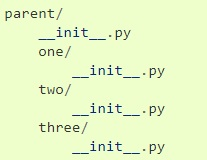
\includegraphics[scale = 0.8]{Recursos/paqueteRegular.jpg}
    \caption{Organización de directorios de un paquete regular}
    \label{PaqueteRegular}
\end{figure}
Cuando se requiere emplear un paquete es necesario primero importarlo; por lo que al importar parent.one (Ver Figura \ref{PaqueteRegular}) se ejecutará implícitamente \mintinline{Python}{parent/__init__.py} y \mintinline{Python}{parent/one/__init__.py}. 
\item \textbf{Paquetes de espacio de nombre (namespace package):} Pertenecen a esta categoría aquellos paquetes compuestos por un conjunto de archivos en un único directorio, donde cada grupo de archivos contribuye con un sub-paquete del paquete padre. A diferencia de los paquetes regulares, los conjuntos pueden estar en diferentes lugares del sistema de archivos, pueden estar en archivos .zip, en la red o cualquier otro lugar que Python busque durante la importación.
\\
Un ejemplo en donde se separa el paquete en dos distribuciones utilizando namespaces sería:
\begin{figure}[H]
    \centering
    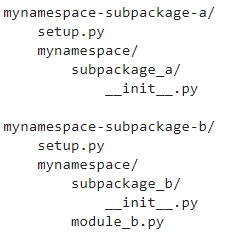
\includegraphics{Recursos/namespacePaquete.jpg}
    \caption{Organización de directorios de un paquete de espacios de nombre}
    \label{namespacePaquete}
\end{figure}
La forma de organizar el paquete utilizada en la Figura \ref{namespacePaquete} no es la única, existen otras formas donde el fichero setup.py, se encuentra en la raíz del paquete, como es el caso de los paquetes con namespace implícito \cite{PEP420}.  El fichero setup.py es aquel que permite la construcción, distribución e instalación de módulos.
\item \textbf{Paquete de importaciones relativas:} Basados en puntos iniciales. Un punto inicial indica una importación relativa, empezando por el paquete actual. Dos o más puntos iniciales indican una importación relativa a los elementos primarios del paquete actual, un nivel por punto después del primero. Por ejemplo, dado el siguiente diseño de paquete:
\begin{figure}[H]
    \centering
    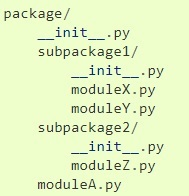
\includegraphics{Recursos/paqueteImportacionRelativa.jpg}
    \caption{Organización de directorios de un paquete de importaciones relativas}
    \label{paqueteIR}
\end{figure}
En \mintinline{Python}{subpackage1/moduleX.py} o \mintinline{Python}{subpackage1/__init__.py}, las siguientes son importaciones relativas válidas:
\begin{figure}[H]
    \centering
    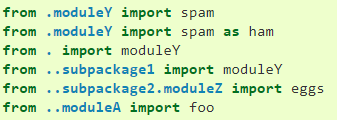
\includegraphics{Recursos/importarRelativamente.png}
    \caption{Ejemplo de importaciones relativas}
    \label{importarIR}
\end{figure}
\end{itemize}
\subsection{Módulos}
Se conoce como modulo a todo fichero o script de Python cuya extensión es .py. Separar el código en módulos permite facilitar el mantenimiento del programa a medida que crezca. Algunos aspectos a tomar en cuenta sobre los módulos serían:
\begin{itemize}
    \item Pueden contener tanto declaraciones ejecutables como definiciones de funciones. Estas declaraciones están pensadas para inicializar el módulo. Se ejecutan únicamente la primera vez que el módulo se encuentra en una declaración import\cite{ModuloPython}.
    \item Cada módulo tiene su propio espacio de nombres, el cual es usado como espacio de nombres global para todas las funciones definidas en su interior.
    \item Para optimizar la importación de módulos el autor del modulo deberá proveer un índice explícito del paquete. Esto se logra cuando el código en el archivo \mintinline{Python}{__init__.py} de un paquete define una lista llamada \mintinline{Python}{__all__.py}, dicha lista debe poseer los nombres de módulos que deberían ser importados cuando se hace \mintinline{Python}{from package import *}\cite{ModuloPython}.
\end{itemize}
\subsection{Tipos de  scripts de configuración del paquete}
\subsubsection{Distutils}
Es un paquete de Python que da soporte, para la creación, distribución e instalación de módulos, los módulos pueden ser hechos únicamente en Python o escritos en C. Distutils como paquete presenta las siguientes funcionalidades:
\begin{itemize}
    \item Soporte para declarar dependencias del proyecto, siendo las dependencias aquellos paquetes o módulos externos necesarios para el funcionamiento del proyecto.
    \item Mecanismos adicionales para configurar cuáles archivos incluir en lanzamientos de código fuente, esto se logra mediante el uso de sistemas de control de versiones.
    \item La capacidad de generar, automáticamente, ejecutables de línea de comandos de Windows en el momento de la instalación, en lugar de tener que compilarlos previamente.
    \item Comportamiento consistente en todas las versiones de Python soportadas por el paquete.
\end{itemize}
Un ejemplo de como estructurar el archivo setup.py que maneja Distutils sería:
\begin{figure}[H]
    \centering
    \begin{minted}{Python}
		from distutils.core import setup
		setup(name='Distutils',
                version='1.0',
                description='Python Distribution Utilities',
                author='Greg Ward',
                author_email='gward@python.net',
                url='https://www.python.org/sigs/distutils-sig/',
                packages=['distutils', 'distutils.command'],)
	\end{minted}
    \caption{Ejemplo de archivo setup.py utilizando el paquete Distutils}
    \label{ejDistutils}
\end{figure}
En la Figura \ref{ejDistutils} es importante resaltar la opción ``packages'' debido a que esta le dice a Distutils que procese (compile, distribuya, instale, etc.) todos los módulos de Python que se encuentran en cada paquete mencionado en la lista de "packages".
\subsubsection{Setuptools}
Es un paquete que contiene una serie de mejoras a las capacidades de Distutils, cuya cualidad principal es permitir que los desarrolladores puedan distribuir paquetes de forma más sencilla, con especial énfasis en paquetes que posean dependencias externas. Esto no implica que distutils sea obsoleto, puesto que setuptools aun se encuentra en desarrollo. A diferencia de su contra parte, las configuraciones requieren de al menos 2 archivos y un paquete, el archivo pyproject.toml; es aquel donde se debe declarar que se empleara Setuptools, este archivo debe poseer la siguiente estructura:
\begin{figure}[H]
    \centering
    \begin{minted}{Python}
		[build-system]
        requires = ["setuptools", "wheel"]
        build-backend = "setuptools.build_meta"
	\end{minted}
    \caption{Ejemplo de archivo pyproject.toml}
    \label{pyproject.toml}
\end{figure}
El archivo setup.cfg es el reemplazo al archivo setup.py y puede conformarse de la siguiente manera:
\begin{figure}[H]
    \centering
    \begin{minted}{Python}
		[metadata]
        name = "mypackage"
        version = 0.0.1

        [options]
        packages = "mypackage"
        install_requires =
        requests
        importlib; python_version == "2.6"
        
        [options.entry_points]
        console_scripts =
        main = mypkg:some_func
	\end{minted}
    \caption{Ejemplo de archivo setup.cfg}
    \label{setup.cfg}
\end{figure}
Como se puede ver en la Figura \ref{setup.cfg} el archivo es bastante similar en estructura al fichero setup.py; no obstante, tiene varias ventajas, ya que los elementos que pertenecen a la opción \mintinline{Python}{install_requires}, son directamente las dependencias del paquete, e incluso al momento de instalar un paquete externo, setuptools actualiza las dependencias necesarias. Para proyectos muy grandes es posible automatizar la busqueda de paquetes, con el fin de que no sea necesario declarar cada paquete en el fichero setup.cfg. 
Las herramientas de configuración admiten la creación automática de scripts tras la instalación mediante "\mintinline{Python}{options.entry_points}". Un paquete que emplee setuptools debe poseer la siguiente estructura de directorios:
\begin{figure}[H]
    \centering
    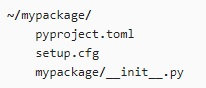
\includegraphics{Recursos/estructuraSetupTools.jpg}
    \caption{Estructura de paquete mediante setuptools}
    \label{estructuraSetupTools}
\end{figure}
El último elemento que requiere Setuptools es el paquete pep517, el cual se puede instalar mediante el instalador de paquetes de python "pip", posteriormente se debe invocar con el comando \mintinline{Python}{python -m pep517.build}.
\subsection{El paquete wheel}
Es un proyecto compatible con distutils y setuptools, que produce un formato de empaquetado binario multiplataforma (llamado ``wheels'' o ``wheel files'' y definido en PEP 427) es decir; la función de wheels es permitir la distribución de paquetes sin importar el sistema operativo empleado \cite{wheel}.
\subsection{Pruebas de regresión mediante modulo unittest}
El objetivo de las pruebas de regresión implementadas mediante el modulo unittest, es probar situaciones donde el codigo deje de funcionar, para encontrar errores en el mismo y solventar problemas en el software, de acuerdo con la documentación oficial existen una serie de pautas a seguir para ejecutar dichas pruebas, las más importantes en el caso del software a desarrollar son:
\begin{itemize}
    \item El conjunto de pruebas se debe hacer a todas las clases, funciones y constantes.
    \item Importar la menor cantidad de módulos posible. Esto minimiza las dependencias externas de las pruebas y también minimiza el posible comportamiento anómalo de los efectos secundarios de importar un módulo.
    \item Maximizar la reutilización del código. En ocasiones, las pruebas variarán en algo tan pequeño como qué tipo de entrada se utiliza.
    \item Asegurar la limpieza después de las pruebas (así como cerrar y eliminar todos los archivos temporales).
    \item Asegurar que todos los valores posibles son probados, incluidos los no válidos. Esto permite que no solo todos los valores válidos sean aceptables, sino que los valores incorrectos se manejen correctamente.
    \item Añadir una prueba explícita para cualquier error descubierto para el código probado. Esto asegurará que el error no vuelva a aparecer si el código se cambia en el futuro.
\end{itemize}
\subsection{Pruebas integradas en cadenas de caracteres de documentación mediante modulo doctest}
Este modulo busca fragmentos de código comentado en el fichero y luego ejecuta esas secciones para verificar que funcionan exactamente como se muestran. Hay varias formas comunes de usar doctest:
\begin{itemize}
    \item Para comprobar que las cadenas de documentación de un módulo estén actualizadas, verificando que todos los ejemplos interactivos sigan funcionando como se documenta.
    \item Para realizar pruebas de regresión verificando que los ejemplos interactivos de un archivo de prueba o un objeto de prueba funcionen como se espera.Esto implica que doctest no sustituye al modulo unittest, al contrario cuando se emplean en conjunto es posible automatizar las pruebas realizadas por doctest.
    \item Para escribir documentación didáctica para un paquete, ilustrada abundantemente con ejemplos de entrada y salida.
\end{itemize}
\section{Proceso de visión estereoscópica}
\subsection{Enfoque clásico}
Era el enfoque más empleado antes del rápido crecimiento de las técnicas basadas en aprendizaje automático, específicamente aquellas apoyadas en ``Deep Learning'' (DL), sin embargo aun se estudia debido a que los conceptos que engloba pueden ser aplicados en el nuevo enfoque. En general la visión estéreo consiste en recuperar las características tridimensionales de una escena a partir de múltiples imágenes tomadas desde varios puntos de vista. De acuerdo con lo propuesto por Barnard y Fischler en 1982, las investigaciones sobre soluciones computacionales para la generalización del problema estéreo siguen un simple paradigma \cite{Barnard1982}, el cual involucra los siguientes pasos:
\subsubsection{Adquisición de imágenes}
Este proceso depende de las condiciones externas del entorno, como la iluminación, el campo o dominio de aplicación, ya que no es igual captar imágenes en entornos cerrados donde la iluminación puede ser constante, que en entornos abiertos donde esta cambiará en el transcurso del día, incluso las condiciones climáticas puedan afectar la imagen, otra condición externa es la existencia de oclusión, la cual puede afectar al momento de interpretar las imágenes y posteriormente realizar satisfactoriamente el paso de correspondencia. El posicionamiento relativo entre cámaras es un factor a tomar en cuenta, ya que este modifica los modelos utilizados en el sistema.
\\
Hasta el momento se han mencionado únicamente los factores externos, sin embargo, al adquirir imágenes estos no son los únicos a tener en cuenta, el tiempo en que se toman las muestras de cada imagen; dependerá de las especificaciones técnicas del hardware empleado, ya que este posee limitaciones en cuanto a velocidad de transmisión y procesamiento, entre otros aspectos ligados a los instrumentos, se encuentra la resolución; que esta asociada al campo de aplicación, el campo de visión o field of view (FOV), que no es mas que el ángulo abarcable por el sensor de una cámara. Además hay ocasiones en las que el ruido presente en las imágenes es  reducido mediante un pre-procesamiento para así mejorar el resultado final del sistema. 
\subsubsection{Modelado de la cámara (geometría del sistema)}
Es una representación de los atributos geométricos y físicos más importantes de las cámaras utilizadas para la visión estéreo. Para poder representar los modelos de las cámaras se emplea el sistema de coordenadas homogéneas y la matriz homogénea, esta es una herramienta introducida por Forest en 1969 para resolver diferentes problemas de gráficos por computador a través de operaciones con matrices. Este tipo de transformaciones son empleadas para determinar en una sola matriz la posición y orientación de un objeto respecto a un sistema de referencia \cite{RSSFernando_homogeneusC}.

Cuando se emplean coordenadas homogéneas en imágenes, cada píxel tiene la siguiente representación:
\begin{equation}
(x, y) \Rightarrow
\begin{bmatrix}
x & y & 1
\end{bmatrix}^{T}
\end{equation}
Mientras que en el caso de una escena tridimensional la representación es:
\begin{equation}
(x, y, z) \Rightarrow
\begin{bmatrix}
x & y & z & 1
\end{bmatrix}^{T}
\end{equation}
Las traslaciones y rotaciones para las coordenadas homogéneas son operaciones lineales realizadas entre matrices, donde la nueva posición de un objeto, sera el producto entre la posición previa y la matriz de transformación. La matriz de transformación homogénea definida por Forest es de dimensiones 4x4 y esta compuesta a su vez por cuatro submatrices (Ecuación \ref{homogeneusMatrix}).
\begin{equation}
    T = \begin{bmatrix}
        \begin{array}{c|c}
                rotaci\acute{o}n & traslaci\acute{o}n\\
                \hline
                perspectiva & escalado
        \end{array}
        \end{bmatrix}
        =
        \begin{bmatrix}
        \begin{array}{c|c}
                3 x 3 & 3 x 1\\
                \hline
                1 x 3 & 1 x 1
        \end{array}
        \end{bmatrix}
\label{homogeneusMatrix}
\end{equation}
No obstante la matriz de transformación para 2D es de dimensiones 3 x 3 y tiene la siguiente representación:
\begin{equation}
    T = \begin{bmatrix}
        \begin{array}{c|c}
                rotaci\acute{o}n & traslaci\acute{o}n\\
                \hline
                perspectiva & escalado
        \end{array}
        \end{bmatrix}
        =
        \begin{bmatrix}
        \begin{array}{c|c}
                2 x 2 & 2 x 1\\
                \hline
                1 x 2 & 1 x 1
        \end{array}
        \end{bmatrix}
\end{equation}
Cuando se emplean coordenadas homogéneas no solo es más eficaz a nivel computacional, ya que permite efectuar cambios en la posición y orientación mediante productos matriciales, estas incluso se pueden convertir en coordenadas convencionales mediante una simple operación de división como en las siguientes expresiones:
\begin{align}
\begin{bmatrix}
x & y & w
\end{bmatrix}^{T} \Rightarrow (x/w, y/w)\label{homogeneus2d}\\
\begin{bmatrix}
x & y & z & w
\end{bmatrix}^{T} \Rightarrow (x/w, y/w, z/w)\label{homogeneus3d}
\end{align}
La ecuación \ref{homogeneus2d} se utiliza para convertir un píxel de una imagen 2D que se encuentra en coordenadas homogéneas a cartesianas, mientras que la ecuación \ref{homogeneus3d} se utiliza en el caso de tres dimensiones.
\\
Para poder estudiar un modelo de múltiples cámaras, es menester comprender  como se aplican las coordenadas homogéneas en uno de una sola cámara. Por este motivo a continuación se presentara el ``modelo de pinhole'', este consiste en que cada punto de un objeto situado en el entorno de trabajo (espacio tridimensional) se proyecta en un punto de un plano denominado plano imagen ó plano de proyección. En la Figura \ref{pinholeModel} ``PP'' es el plano de proyección y ``COP'' se refiere al centro de proyección o centro óptico de la cámara. El punto en la escena 3D se denota como $p^{M}$, dicho punto se encuentra en las coordenadas del mundo $p^{M}$ $(x, y, z)$ y su proyección en el plano de imagen se denota como $p^{I}$ $(x', y')$ y corresponde con la intersección entre la linea que une $p^{M}$ y COP con el plano de imagen, además a la distancia entre el plano de proyección y COP se le conoce como distancia focal. 
\begin{figure}[H]
    \centering
    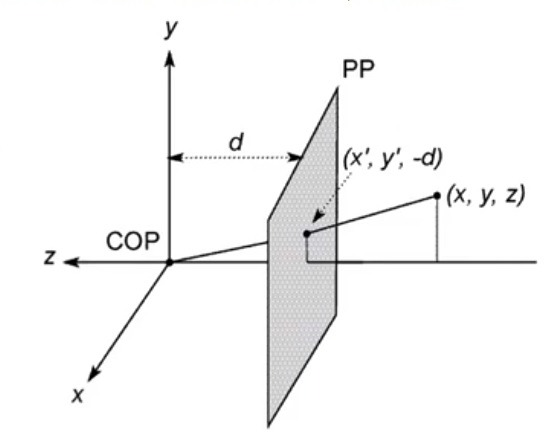
\includegraphics[scale=0.5]{Recursos/pinholeModel.jpg}
    \caption{Modelo de cámara pinhole}
    \label{pinholeModel}
\end{figure}
La razón del porque en el modelo presentado en la Figura \ref{pinholeModel} el plano de proyección se encuentra por delante del lente (a pesar de que en la realidad la luz ingresa a través del punto focal y luego impacta con el plano de imagen) es porque matemáticamente es más conveniente, debido a que de esta forma las imágenes no son invertidas.

Utilizando el teorema de Tales es posible determinar las proyecciones de los puntos en el plano de forma tal que se cumple la siguiente ecuación:
\begin{equation}
    (X, Y, Z) \longrightarrow (-d\frac{X}{Z}, -d\frac{Y}{Z}, -d)  \label{convert3Dto2Dpinhole}
\end{equation}
La operación realizada en la ecuación \ref{convert3Dto2Dpinhole}, permite proyectar los puntos del espacio 3D en el plano de imagen, dicha operación puede ser realizada mediante coordenadas homogéneas de la siguiente forma:
\begin{align}
            \begin{bmatrix}
            1 & 0 & 0 & 0\\
            0 & 1 & 0 & 0\\
            0 & 0 & 1/f & 0
            \end{bmatrix}
            \begin{bmatrix}
            x\\
            y\\
            z\\
            1
            \end{bmatrix}
            =
            \begin{bmatrix}
            x\\
            y\\
            z/f\\
            \end{bmatrix} \Rightarrow \left(-f\frac{X}{Z}, -f\frac{Y}{Z}\right)\label{convert3Dto2Dperspective}
\end{align}
A la forma en la que se proyecta en la ecuación \ref{convert3Dto2Dperspective} se le conoce como proyección de perspectiva y esta llega al mismo resultado que el de la ecuación \ref{convert3Dto2Dpinhole}, ya que $f$ es la distancia focal.
\\
El modelo de dos cámaras o modelo estéreo, es una extrapolación del modelo de pinhole. En general se pueden tener 3 casos en función de cómo se encuentren orientados los ejes de ambas cámaras: disposición convergente, disposición alineada y la disposición divergente, la tercera no permite llevar a cabo un análisis estéreo. En la figura \ref{estereoSystemParallel}, se puede observar el modelo geométrico de dos cámaras  cuando sus ejes ópticos son paralelos, a continuación se listan cada uno de los elementos relevantes:
\begin{itemize}
\item \textbf{Linea base:} es la distancia que separa los dos centros ópticos de ambas cámaras. Se denota B.
\item \textbf{distancia focal:} la distancia entre el plano de imagen y los centros ópticos. Se denota $f$.
\item\textbf{ El punto P:} corresponde con la distancia Z en las coordenadas de los sistemas de cámaras, siempre es medida hasta el centro de proyección (COP) de cada cámara. 
\item \textbf{Plano epipolar de un punto P en el espacio:} En la Figura \ref{estereoSystemParallel3D} se observa el mismo sistema pero con tres dimensiones, en este el plano que contiene el punto P y cada uno de sus centros ópticos $COP_{L}$ y $COP_{R}$ es conocido como el plano epipolar.
\item\textbf{ Linea epipolar:} hay una por cada punto ($p_{l}$ y $p_{r}$), en el caso de la Figura \ref{estereoSystemParallel3D} solo existe una linea debido a que esta es la intersección del plano epipolar con cada una de las imágenes.
\end{itemize}
\begin{figure}[H]
     \centering
     \begin{subfigure}[b]{0.4\textwidth}
        \centering
        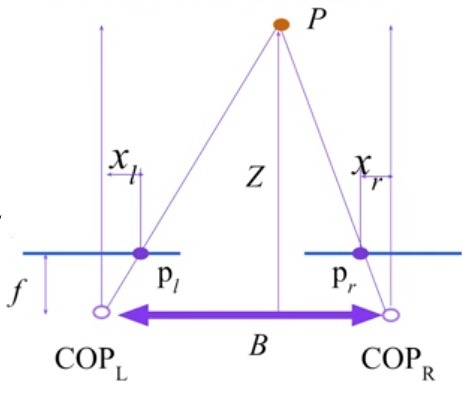
\includegraphics[scale=0.5]{Recursos/stereoGeometry.jpg}
        \caption{Representación del modelo de ejes alineados en el plano}
        \label{estereoSystemParallel}
     \end{subfigure}
     \hfill
     \begin{subfigure}[b]{0.4\textwidth}
         \centering
        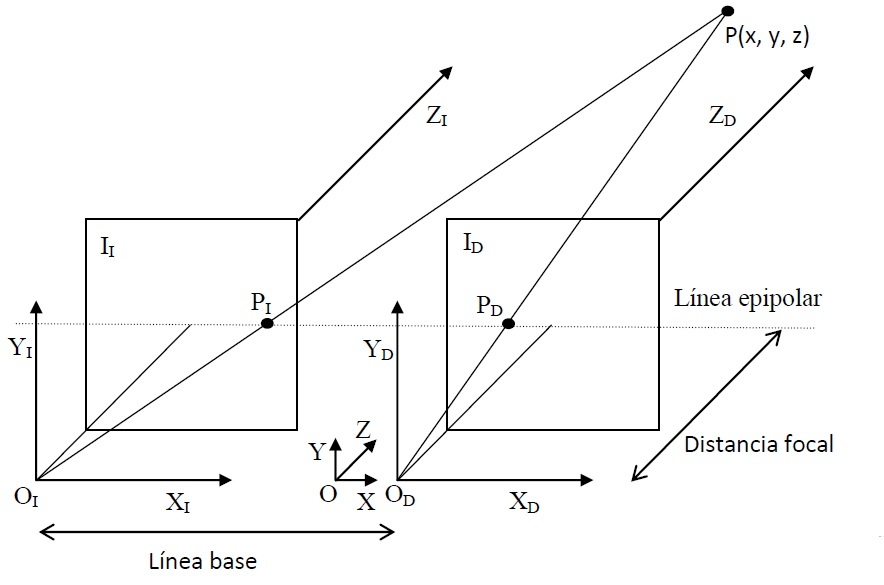
\includegraphics[scale=0.3]{Recursos/stereoGeometry3D.jpg}
        \caption{Representación del modelo de ejes alineados en el espacio}
        \label{estereoSystemParallel3D}
     \end{subfigure}
     \hfill
\caption{Modelo estéreo}
\label{stereoMODEL}
\end{figure}
Para el modelo de ejes alineados presentado en las Figuras \ref{estereoSystemParallel} y \ref{estereoSystemParallel3D}, es posible calcular las coordenadas de las proyecciones del punto P sobre cada una de las cámaras, utilizando el teorema de triángulos similares, de tal forma que su posición en el espacio estará dada por: 
\begin{align}
x_{p} = \frac{x_{l}\cdot B}{x_{l} - x_{r}}\\
y_{p} = \frac{y_{l}\cdot B}{x_{l} - x_{r}}\\
z_{p} = \frac{f\cdot B}{x_{l} - x_{r}}
\end{align}
La diferencia $x_{l} - x_{r}$ es conocida como disparidad.
\subsubsection{Extracción de las características}
En este paso se extraen los elementos que identifican a una imagen. De estos elementos, a su vez se tienen que extraer algunos atributos, los cuales se utilizarán en el siguiente paso. Por lo tanto, este paso está muy ligado al de correspondencia y al ser el paso de correspondencia el más importante de todos, primero se suele decidir qué método utilizar al realizar la correspondencia entre imágenes y según las características que se empleen, éstas serán las que se extraigan de las imágenes. Existen dos clases de técnicas para determinar la correspondencia entre dos imágenes estereoscópicas: las técnicas basadas en el área (“area-based”) y las técnicas basadas en las características (“feature-based”).
\\
Las técnicas basadas en área emplean la correlación cruzada entre patrones de intensidad en la vecindad local o vecindario de un píxel en una imagen, con patrones también de intensidad en una vecindad correspondiente a un píxel en la otra imagen del par estereoscópico. Por tanto, las técnicas basadas en el área utilizan la intensidad de los píxeles como característica esencial. Por otro lado las basadas en características se toman representaciones simbólicas obtenidas de las imágenes de intensidad en vez de utilizar las intensidades directamente. Algunas de las características cuyo uso está más extendido son: puntos de borde aislados, cadenas de puntos de bordes o regiones delimitadas por bordes.
\subsubsection{Correspondencia de las imágenes (características)}
Este paso puede tener como entradas pixeles o caracteristicas, de modo que con estas se calculen las profundidades a partir de la disparidad existente, la disparidad se puede entender como la diferencia entre las posiciones de las proyecciones en las imagenes y es representada por la siguiente expresión:
\begin{equation}
d = x_{l} - x_{r} = \frac{f\cdot B}{z_{p}}
\end{equation}
El problema de la disparidad es que existe cierta ambiguedad entre las imagenes. Habra puntos de caracteristicas similares en ambas imagenes y solo uno de esos puntos en cada uno de ellas son correspondientes entre si. De aqui la importancia del paso previo y es que en aquel paso se determina el conjunto inicial de caracteristicas faciles de distingir del resto de pixeles en las imagenes (esquinas, bordes, etc) y que serviran para inicializar el proceso de correspondencia. En la correspondencia se filtraran por medio de un conjunto de restricciones que vayan delimitando y reduciendo la ambiguedad de los posibles pares de proyecciones que se iran conjugando.
\\
Las restricciones pueden ser de tres tipos:
\begin{itemize}
\item\textbf{ Restricciones geométricas}: son aquellas impuestas por el sistema de visión estéreo. Entre todas ellas se destacan la restricción epipolar, la cual consiste en que las imágenes de una misma entidad 3D deben proyectarse sobre la misma línea epipolar. Esta restricción se deriva de la geometría de las cámaras y requiere que las mismas estén alineadas. Y la restricción de unicidad implica, que para cada característica en una imagen debe haber una única característica en la otra imagen, salvo que se produzca una oclusión y no haya correspondencia de alguna característica.
\item \textbf{Físicas y basadas en propiedades de la escena:} Dependen de la naturaleza de los objetos. Hacen  referencia a iluminaciones, superficies, formas, etc. Algunas de las mas usadas son la de ordenación, donde dadas dos características en una determinada imagen, por ejemplo la izquierda, situada una a la derecha de la otra, esta restricción supone que este mismo orden se mantiene en la imagen derecha para sus respectivas características homólogas. Y la restricción de continuidad límite de disparidad, asume que las variaciones de disparidad en la imagen son generalmente suaves, es decir que si consideramos un mapa de disparidad éste se presenta continuo salvo en unas pocas discontinuidades.
\end{itemize}
\subsubsection{Determinación de la distancia (profundidad)}
Una vez que se ha hecho corresponder los elementos que aparecen en la imagen izquierda con los elementos en la imagen derecha, la determinación de la profundidad es un proceso relativamente sencillo, reduciéndose a una simple triangulación. Sin embargo en algunas ocasiones, cuando se intenta hallar la distancia a la que se encuentra una característica, se presentan algunas dificultades debidas a una falta de precisión o una escasa fiabilidad cuando se intentó encontrar la correspondencia.
\\
Debido a las restricciones de epipolares, las proyecciones de un objeto real en cada una de las imágenes solamente se diferenciarán en la coordenada x de sus sistemas de referencia relativos, ya que la coordenada y será idéntica. De forma que dos elementos de las imágenes, que representan al mismo objeto, solo tendrán desplazamiento horizontal. Exactamente este desplazamiento es lo que hemos llamado disparidad.
\subsubsection{Interpolación}
Es un paso que no siempre es aplicado y se utiliza cuando se emplea el enfoque basado en características, ya que es cuando la información sobre distancias puede ser
insuficiente. Normalmente las aplicaciones requieren de mapas de profundidad más o
menos densos. Que un mapa de profundidad sea denso significa que hay mucha
información sobre la distancia a la que se encuentran los elementos de la escena por unidad de superficie, frente a un mapa de superficie disperso en el que la información que se dispone por unidad de superficie es menor. La densidad de un mapa es un valor que se puede cuantificar más o menos, pero que se considere lo suficientemente denso o no depende únicamente de la aplicación. Por ejemplo en el caso de un mapa de disparidad, donde cada píxel de la imagen capturada se disponga de un valor de la distancia a la que se encuentra ese punto de la cámara en la escena
tridimensional, se puede considerar muy denso.
\\
Sin embargo, en el caso de los métodos de correspondencia basados en características se suele llegar a mapas de disparidad dispersos, porque las características que tienen las imágenes suelen estar diseminadas y distribuidas irregularmente. Los métodos de correspondencia basados en el área son más apropiados que los métodos de correlación basados en las características si se quiere obtener un mapa de profundidades denso, aunque la información de los métodos basados en las características sea más fiable. La información de los métodos basados en el área suele ser menos fiable por problemas tales como la existencia de zonas donde el brillo es muy uniforme y no se puede realizar una correspondencia con certeza.
\\
Para solucionar estos problemas se emplea la interpolación, interpretando al mapa de disparidad, como un muestreo de una función de profundidad continua y utilizando el método de interpolación tradicional para hallar una función continua que la aproxime. Así se obtendría una función con la que obtener la profundidad para cualquier punto de espacio tridimensional, consiguiendo transformar un mapa de profundidad disperso en denso. Algunos de los métodos empleados para interpolar son: la interpolación de Lagrange, la interpolación de Hermite, interpolación mediante Splines, o mediante wavelets.
\subsection{Enfoque basado en Aprendizaje}
Los métodos basados en el aprendizaje pueden separarse en dos clases:
\begin{itemize}
    \item Las que imitan las técnicas de correspondencia estéreo, aprendiendo explícitamente cómo hacer coincidir los píxeles de la imagen de entrada de una cámara con los de la otra, para luego convertirlos en un flujo óptico o un mapa de disparidad y finalmente transformar cualquiera de los anteriores en su valor respectivo de profundidad. Esta estrategia posee tres módulos básicos: módulo de extracción, coincidencia de características y un modulo de agregación de costos, por ultimo se realiza la estimación de disparidad / profundidad (Ver Figura \ref{mimicStereo}). Es importante resaltar que esta estrategia se caracteriza porque cada modulo es entrenado independientemente de los otros \cite{laga2020survey}.
    \begin{figure}[H]
        \centering
        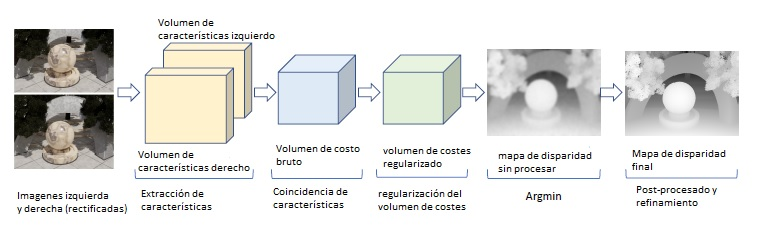
\includegraphics[scale=0.6]{Recursos/mimicStereo.jpg}
        \caption{Los componentes básicos para un proceso de correspondencia estéreo.}
        \label{mimicStereo}
    \end{figure}
    \item Las que resuelven el problema de correspondencia utilizando una ``pipeline'' o cadena de procesos que se puede entrenar de extremo a extremo. Esta categoría puede ser subdividida en dos tipos: aquellos métodos que formularon la estimación de profundidad como un problema de regresión. En otras palabras, el mapa de profundidad se infiere directamente de la entrada sin características que coincidan explícitamente a través de las vistas de ambas cámaras. Estos métodos son simples y rápidos en tiempo de ejecución, sin embargo; requieren una gran cantidad de datos de entrenamiento, el cual puede ser difícil de obtener. Por otro lado lo métodos que pertenecen a la segunda clase, imitan el canal de emparejamiento estéreo tradicional rompiendo el problema en etapas compuestas por bloques diferenciables y permitiendo así la formación de principio a fin.
\end{itemize}
\section{Fundamentos del aprendizaje profundo o deep learning}
El aprendizaje profundo, es una rama del aprendizaje automático ó machine learning, que se caracteriza por poseer un conjunto de datos de entradas, ejemplos de una salida esperada por el sistema y una forma de medir cuando un algoritmo esta realizando adecuadamente su trabajo, este ultimo elemento es necesario, ya que permite determinar la distancia entre la salida actual del algoritmo y la salida esperada, la medición de la salida es usada como una señal de realimentación para así ajustar la forma en que el algoritmo funciona. A este ajuste se le conoce como ``aprendizaje''.
\\
La idea base de este sub-campo del machine learning, nace del interés de replicar en sistemas computacionales el comportamiento de las neuronas presentes en los seres vivos, las cuales son responsables del aprendizaje y sus inicios datan de  1958 cuando Rosenblatt desarrollo el perceptron (Ver Figura \ref{perceptron}).
\begin{figure}[H]
    \centering
    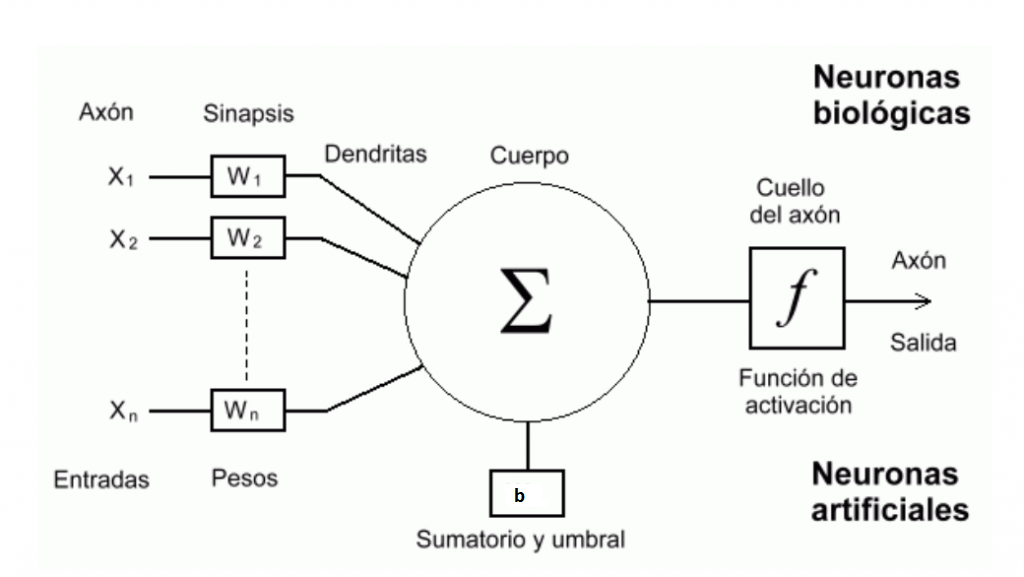
\includegraphics[scale=0.35]{Recursos/perceptron.png}
    \caption{Comparación de una neurona biológica con una neurona artificial}
    \label{perceptron}
\end{figure}
En comparación con otras técnicas de aprendizaje automático, que normalmente se basan en varias
etapas de pre-procesamiento para extraer características en las que se pueden construir clasificadores, el enfoque de aprendizaje profundo
generalmente se entrena de un extremo a otro, yendo directamente desde píxeles sin procesar hasta los resultados finales deseados \cite{Szeliski2020}.
\subsection{Elementos de las redes neuronales}
\subsubsection{Pesos y capas}
Una red neuronal profunda extiende la idea del perceptron (Ver Figura \ref{perceptron}) que utiliza una única neurona, a un grafo compuesto por miles de neuronas interconectadas. En la Figura \ref{NeuralNetworkArq} cada circulo corresponde con una neurona cuya salida estará dada por la siguiente expresión:
\begin{equation}
    s_{i} = w_{i}^{T} x_{i} + b_{i} \label{ponderedSum}
\end{equation}
el resultado de las sumas ponderadas (ecuación \ref{ponderedSum}) de cada neurona pasa por una función de activación no linear que redistribuirá los valores en un rango acotado:
\begin{equation}
    y_{i} = h(s_{i})
\end{equation}
En la ecuación \ref{ponderedSum}, los valores de $x_{i}$ son las entradas de de la i-esima neurona, $w_{i}$ y $b_{i}$ son parámetros que se van ajustando en el proceso de aprendizaje y corresponden con los pesos y el bias respectivamente. 
\begin{figure}[H]
    \centering
    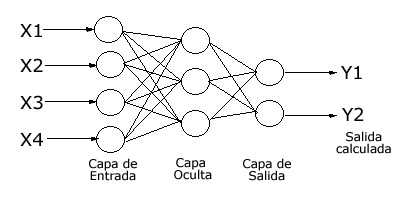
\includegraphics{Recursos/NeuralNetwork.jpg}
    \caption{Arquitectura de una red neuronal multicapas}
    \label{NeuralNetworkArq}
\end{figure}
A las capas de la Figura \ref{NeuralNetworkArq} se les conoce como ``fully conected'' (FC), debido a que todas las entradas de una capa están conectadas a todas sus salidas. Dado que las redes neuronales suelen estar organizadas en capas consecutivas, es posible agrupar cada neurona dentro de una capa en un vector, cuya combinación lineal se escribe como:
\begin{equation}
    s_{l} = w_{l}^{T} x_{l}
\end{equation}
donde $x_{l}$ son las entradas a la capa $l$, $W_{l}$ es una matriz de peso y $s_{l}$ es la suma ponderada, a la que se aplica una función de activación:
\begin{equation}
    x_{l+1} = y_{l} = h(s_{l)}
\end{equation}
Una red que consiste únicamente en capas FC, se le conoce como perceptron multicapa. 
\subsubsection{Funciones de activación}
Las funciones de activación se usan para propagar la salida de los nodos de una capa hacia la siguiente capa. Además este tipo de funciones permiten incorporar al modelo no linealidades, que permitirán que este se ajuste a cualquier distribución de datos. Algunas de las funciones de activación más comunes son:
\begin{itemize}
    \item \textbf{función logística o sigmoidea:} Este tipo de funciones permiten mitigar el efecto de ``outliers'' (valores atípicos que son numéricamente distantes del resto de los datos) en el entrenamiento del modelo. La imagen de este tipo de funciones suele estar contenida en los intervalos [0, 1]. Por lo que valores muy extremos siempre estarán cerca de los límites del intervalo de esa imagen. Su ecuación esta dada por:
    \begin{equation}
        h(x) = \frac{1}{1 + e^{-x}}
    \end{equation}
    \item \textbf{Tangente hiperbólica:} Es una función no lineal cuyo rango normalizado se encuentra entre [-1, 1] y su ventaja  es que puede manejar más fácilmente los números negativos. Su ecuación esta dada por:
    \begin{equation}
        h(x) = \frac{e^{x} - e^{-x}}{e^{x} + e^{-x}}
    \end{equation}
    \item \textbf{ReLu o rampa:} Es una de las funciones mas utilizadas en CNN y en redes profundas debido a que con ella se logran mejores resultados que con la sigmoidea y la hiperbólica, ya que en el procesamiento de imágenes los valores negativos  no son importantes y por lo tanto se establecen en 0. Pero los valores positivos después de la convolución deben pasar a la siguiente capa. En cambio si se emplean la hiperbólica o la sigmoidea,  la información se pierde ya que ambas funciones modificarán las entradas a un rango muy cerrado. Su ecuación esta dada por:
    \begin{equation}
        h(x) = max(0,x)
    \end{equation}
\end{itemize}
\subsubsection{Funciones de error}
Como se ha podido observar el proceso de aprendizaje de una red neuronal es de carácter iterativo, ya que, lo que se busca es ajustar un modelo a un conjunto de datos. Las funciones de error permiten medir la distancia a la que se encuentra un modelo del objetivo, de esta forma es posible tomar medidas adecuadas en la siguiente iteración, para así reducir el error hasta alcanzar valores mínimos. Dependiendo de la tarea a realizar se utilizan diferentes funciones de error. 
\\
Por ejemplo, en el caso de redes que utilicen como datos de entrada mapas de profundidad (mapas de disparidad) ó imágenes sin ruido, se suele realizar una regresión matemática que ajuste al modelo, por lo que es común utilizar la norma L2 como función de error
\begin{equation}
    E(w) = \sum_{n} E_{n}(w) = - \sum_{n} ||y_{n} - t_{n}||^{2}
\end{equation}
donde $y_{n}$ es la salida de la red para la muestra n y $t_{n}$ es el valor objetivo. Sin embargo, si son pocos los ``outliers'' en los datos de entrenamiento, o si los errores graves no son tan dañinos como para merecer una penalización cuadrática, se pueden utilizar normas más robustas como la L1
\begin{equation}
    E(w) = \sum_{n} E_{n}(w) = - \sum_{n} ||y_{n} - t_{n}||
\end{equation}
Cabe resaltar que no son las únicas funciones de error utilizadas en el campo de visión estéreo, pues existen variaciones, como en el trabajo realizado por Sizhang Dai y Weibing Huang en marzo del 2020 \cite{dai2020atvsnet} donde usan el error absoluto medio.
\subsubsection{Técnicas para la optimización de la red}
Cuando se entrena una red se emplean diversas técnicas que mejoran los resultados de la misma, o permiten que las redes neuronales no sufran de ``overfitting'' (sobre ajuste) para así poder generalizar mejor. A continuación se detallaran algunas de las técnicas mas empleadas así como lo es el ``dropout'' y la normalización del lote.
\begin{itemize}
    \item \textbf{Regularización:} es una técnica que surge cuando se optimizan los pesos dentro de una red neuronal, los pesos se vuelven más pequeños, a este fenómeno se le conoce como decaimiento de los pesos y es un problema debido a que al pasar por la función de activación un valor de suma ponderada muy cercano a 0, es mucho mas difícil para el algoritmo del descenso al gradiente desplazar el valor de ese peso a su óptimo. En la practica, valores muy pequeños se traducen a coeficientes con muchos decimales y esto es sinónimo de ``overfitting'', para solucionar esto se aplica regularización a la función de error, lo que penaliza en mayor medida a los pesos con largos coeficientes. A continuación se presentan las regularizaciones L1 y L2 respectivamente.
    \begin{align}
          E(w)_{L1} = - \sum_{n} ||y_{n} - t_{n}|| + \lambda \sum_{i} |w_{i}|\\
          E(w)_{L2} = - \sum_{n} ||y_{n} - t_{n}|| + \lambda \sum_{i} w_{i}^{2}\\
    \end{align}
    El valor de $\lambda$ corresponde con cuanto se quieren penalizar los coeficientes de los pesos $w_{i}$.
    \item \textbf{Dropout:} es una técnica aplicada a todas las neuronas de una capa, consiste en que a cada neurona de la capa en cuestión tendrá asociada una probabilidad de desactivación que puede estar entre 0 y 100\%, por lo que la red tendría un funcionamiento como el de la Figura \ref{dropout}.
    \begin{figure}[H]
        \centering
        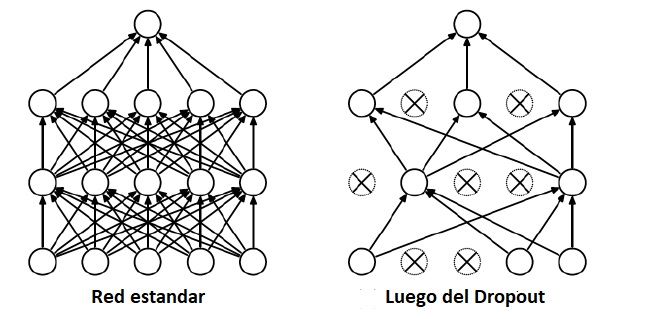
\includegraphics[scale=0.7]{Recursos/Dropout.jpg}
        \caption{Efecto del Dropout en el entrenamiento}
        \label{dropout}
    \end{figure}
    Colocar neuronas aleatoriamente a cero inyecta ruido en el proceso de formación y también evita que la red se especialice demasiado neuronas a muestras o tareas particulares, las cuales pueden ayudar a reducir el sobreajuste y mejorar la generalización.
    \item \textbf{Aumento del conjunto de datos:} Otra técnica poderosa para reducir el ajuste excesivo es agregar más muestras de entrenamiento perturbando las entradas y / o salidas de las muestras que ya han sido recolectadas. Esta técnica es eficaz en tareas de clasificación de imágenes, ya que es caro obtener ejemplos etiquetados, y también dado que las clases de imágenes no deben cambiar bajo pequeñas perturbaciones.
\end{itemize}
\subsubsection{Algoritmo de backpropagation}
Propuesto en 1986 por  Rumelhart, Hinton y Williams, es el responsable de que una red neuronal sea capaz de auto ajustar sus parámetros para así aprender una representación interna de la información que estaba procesando. Para su ejecución se requiere de un algoritmo conocido como descenso al gradiente, el cual consiste en que en cada iteración del entrenamiento se evalué el error del modelo y se calculen las derivadas parciales (gradientes) de dicho error, los gradientes indicaran la pendiente de la función hacia donde el error incrementa, por lo que para reducir el error en cada iteración, es necesario substraer el vector de gradientes al resultado final. 
\\
No obstante, debido a la estructura de una red neuronal, los valores de los parámetros en las capas posteriores dependen de las capas previas y a su vez de las conexiones entre neuronas, por lo que calcular el gradiente de forma directa no es una opción, la solución es utilizar el descenso del gradiente para optimizar la función de coste (función de error) empleando la técnica de de backpropagation para calcular el vector de gradientes dentro de la complejidad de la arquitectura de la red. 
\\
El funcionamiento de este algoritmo parte de analizar desde el final de la red con la señal de error hacia las primeras capas, la razón del porque se va desde la ultima capa hacia la primera capa, es que en una red neuronal el error de las capas anteriores depende directamente del error de las capas posteriores, teniendo en cuenta este hecho, es posible determinar cual es el efecto de cada neurona en el resultado final mediante la retro propagación de errores, de este modo es posible computar cuanto hay que modificar cada parámetro en cada neurona. Además una vez aplicados los errores a las neuronas de la capa de turno se puede proceder a repetir el mismo proceso previo como si este fuera el error de la red; es decir, asumiendo que la capa de turno es la nueva ultima capa, así aplicar backpropagation es operar siempre de forma recursiva capa tras capa moviendo el error hacia atrás. Entonces al alcanzar la primera capa se habrá obtenido cual es el error para cada neurona y para cada uno de sus parámetros, dichos errores son usados para calcular las derivadas parciales de cada parámetro de la red, conformado así el vector de gradientes al cual se le aplica el descenso al gradiente para lograr minimizar el error. 
\subsection{Redes neuronales convolucionales ó Convolutional Neural Networks (CNN)}
Es una arquitectura de red empleada en el procesamiento de imágenes, cuya principal ventaja respecto a las redes estudiadas previamente, es su eficiencia al momento del entrenamiento, ya que la cantidad de parámetros a ajustar se reduce considerablemente. A diferencia de una red de capas FC las capas de las redes CNN consisten en un conjunto de filtros que se van ajustando a medida que avanza el aprendizaje, cada filtro suele ser pequeño espacialmente (tanto en ancho como en alto)  respecto a las dimensiones de la imagen de entrada, pero estos se extienden a través de todas las dimensiones del volumen de entrada, se le conoce como volumen de entrada debido a que una imagen con los 3 canales (RGB) corresponde con un tensor de dimensiones  $WxHxD$ (ancho x alto x profundidad). Al introducir una imagen en la red se desliza (mas precisamente, se realiza la convolución) cada filtro a través de todo el ancho y alto del volumen de entrada y se calculan los productos escalares entre las entradas del filtro y la entrada en cualquier posición.  A medida que se desliza el filtro sobre el ancho y el alto del volumen de entrada, se producirá un mapa de activación bidimensional o mapa de características, que da las respuestas de ese filtro en cada posición espacial (Ver Figura \ref{fowardPassCNN}).
\begin{figure}[H]
    \centering
    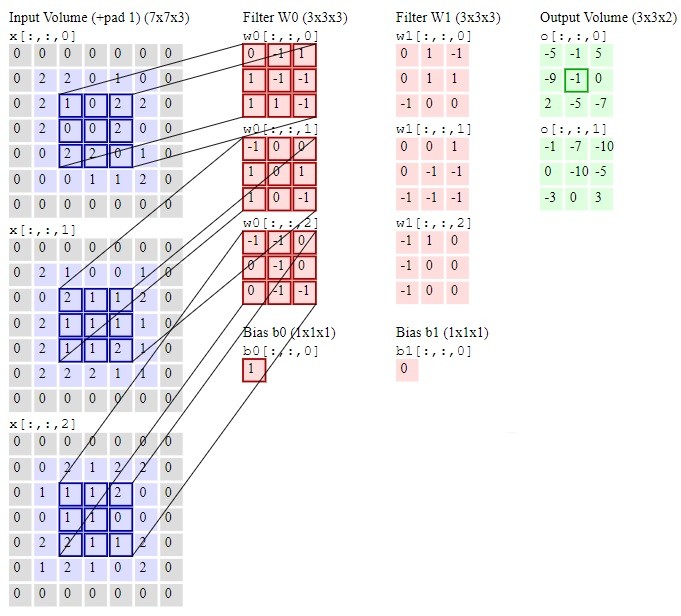
\includegraphics[scale=0.7]{Recursos/fowardPassCNN.jpg}
    \caption{Convolución entre el volumen de entrada de dimensiones 7x7x3 y dos filtros de dimensiones 3x3x3}
    \label{fowardPassCNN}
\end{figure}
De forma intuitiva, la red aprenderá filtros que se activan cuando ven algún tipo de característica visual, como un borde de alguna orientación o una mancha de algún color en la primera capa, o eventualmente patrones enteros en forma de panal o rueda en capas superiores de la red. De este modo se tendrá un conjunto completo de filtros en cada capa, en lugar de neuronas y cada uno de ellos producirá un mapa de activación bidimensional separado. Se Apilaran estos mapas de activación a lo largo de la dimensión de profundidad generando así el volumen de salida\cite{CS231n}.
\\ 
En las CNN se suelen emplear dos tipos de capas, aquellas donde se realiza la convolución, las cuales fueron descritas previamente y las capas de agrupación o ``polling layers'', estas son insertadas periódicamente entre capas de convolución con el fin de reducir progresivamente el tamaño espacial de la representación para así disminuir la cantidad de parámetros y cálculos en la red y, por lo tanto, controlar también el ``overfitting''. La capa de agrupación funciona de forma independiente  en cada segmento de profundidad de la entrada y la redimensiona espacialmente, utilizando la operación MAX. La forma más común es una capa de agrupación con filtros de tamaño 2x2 aplicados con un paso de 2, por lo que con estos parámetros la operación MAX tomaría el valor máximo entre 4 números en una región de 2x2 (Ver Figura \ref{maxPooling}). De manera más general, la capa de agrupación:
\begin{itemize}
    \item Acepta un volumen de dimensiones $W_{1}xH_{1}xD_{1}$
    \item Requiere dos hiperparámetros:
    \begin{itemize}
        \item Su extensión espacial ``F''
        \item El paso o zancada ``S''
    \end{itemize}
    \item Produce un volumen $W_{2}xH_{2}xD_{2}$ donde:
    \begin{itemize}
        \item $W_{2}$ $=$ $(W_{1}-F)/S+1$
        \item $H_{2}$ $=$ $(H_{1}-F)/S+1$
        \item $D_{2}$ $=$ $D_{1}$
    \end{itemize}
    \item Introduce cero parámetros ya que calcula una función fija de la entrada
    \item Para las capas de agrupación, no es común rellenar la entrada con relleno de ceros, como en el caso de una capa de convolución.
\end{itemize}
\begin{figure}[H]
    \centering
    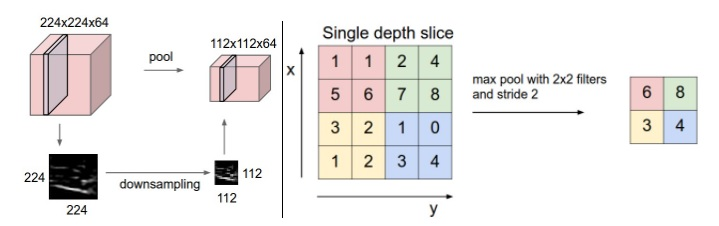
\includegraphics[scale=0.6]{Recursos/maxPolling.jpg}
    \caption{Capa de agrupación para un volumen de entrada de 224x224x64 con F = 2, P = 2 y un volumen de salida de 112x112x32}
    \label{maxPooling}
\end{figure}
\subsection{Hiperparámetros de las redes CNN}
Son las variables que rigen el proceso de entrenamiento en sí, es decir; son variables de configuración. En el caso de las capas de convolución se tienen:
\begin{enumerate}
    \item La profundidad del volumen de salida: corresponde a la cantidad de filtros a usar en cada capa y se identifica por $D_{n}$ donde $n$ es el numero de la capa en cuestión. Sin embargo, también puede identificarse mediante $K$.
    \item El campo receptivo de la neurona: es equivalente al tamaño del filtro y se identifica mediante $F$.
    \item El paso o zancada: corresponde con la cantidad de pixeles por las que se desliza el filtro al momento de realizar la convolución, se identifica mediante la letra $S$. Por ejemplo cuando el paso es 1, los filtros se desplazan un píxel a la vez. En el caso de ser 2 los filtros saltan 2 píxeles a la vez a medida que se deslizan por el volumen de entrada, de esta forma se producirán volúmenes de salida más pequeños espacialmente.
    \item El relleno: hay casos donde sera conveniente rellenar el volumen de entrada con ceros alrededor del borde, como es el caso de la Figura \ref{fowardPassCNN}. Por lo tanto el tamaño del relleno de ceros es un hiperparámetro que  permitirá controlar el tamaño espacial de los volúmenes de salida, aunque su aplicación más común es la de preservar exactamente el tamaño espacial del volumen de entrada para que el ancho de entrada y salida y la altura sean los mismos.
    \item Dilatación: este parámetro permite tener filtros que tengan espacios entre cada celda, por ejemplo; en el caso de una dimensión un filtro $w$ de tamaño 3 calcularía sobre la entrada $x$ lo siguiente:  $w [0] * x [0] + w [1] * x [1] + w [2] * x [2]$ . Este es en el caso de que no exista dilatación (dilatación = 0). Para la dilatación = 1, el filtro calcularía $w [0] * x [0] + w [1] * x [2] + w [2] * x [4]$; En otras palabras, hay una brecha de 1 entre las aplicaciones.  Esto puede ser muy útil en algunas configuraciones para usar junto con filtros de dilatación 0 porque le permite fusionar información espacial a través de las entradas de manera mucho más agresiva con menos capas.
\end{enumerate}
De acuerdo con los hiperparámetros, una capa convolucional se caracteriza por:
\begin{itemize}
    \item Acepta un volumen de dimensiones $W_{1}xH_{1}xD_{1}$.
    \item Requiere 4 hiperparámetros:
    \begin{itemize}
        \item El numero de filtros ``K''
        \item La extensión de los filtros ``F''
        \item El paso ``S''
        \item la cantidad de relleno ``P''.
    \end{itemize}
    \item Produce un volumen $W_{2}xH_{2}xD_{2}$ donde:
    \begin{itemize}
        \item $W_{2}$ $=$ $(W_{1} - F + 2P)/S+1$
        \item $H_{2}$ $=$ $(H_{1} - F + 2P)/S+1$
        \item $D_{2}$ $=$ $K$
    \end{itemize}
\end{itemize}
%

%==================================================================
\chapter{DESCRIPCIÓN DEL SISTEMA DE ADQUISICIÓN DE DATOS}\label{CAP:hardware}
%\markboth{Tu Segundo Capítulo}{Tu Segundo Capítulo}%
En este capítulo se detallarán las herramientas necesarias para el desarrollo del paquete, como lo son el editor de texto, servidores externos para el entrenamiento del o los modelos, paquetes necesarios para la documentación, distribución, \textit{testing} y cualquier elemento adicional que sea fundamental para su funcionamiento. A su vez, se especificará la arquitectura del software, haciendo énfasis en los patrones de diseño aplicados y la función de cada módulo o submódulo programado.
\section{Macro estructura del paquete}
Para el desarrollo del paquete se buscó que las piezas de código fuesen independientes, con el fin de lograrlo se separaron en dos módulos distintos las funciones de reconocimiento y estéreo, los cuales como se puede observar en la Figura \ref{modos_func_paquete}, son capaces de obtener resultados finales acordes a su función para luego unificar sus resultados y obtener la posición de los objetos en la escena. Adicionalmente, en la Figura \ref{modos_func_paquete} se puede apreciar que las entradas de este paquete son imágenes o vídeos, en el caso del módulo de reconocimiento es suficiente con una cámara, no obstante; cuando se le agrega estéreo es necesario poseer un hardware adecuado, del cual se profundizara en el siguiente capítulo, también se precisó el uso de una plataforma (Google colab) para realizar el entrenamiento del o los modelos de reconocimiento, a continuación se profundizará en las cualidades de dicha plataforma.
\begin{figure}[H]
    \centering
    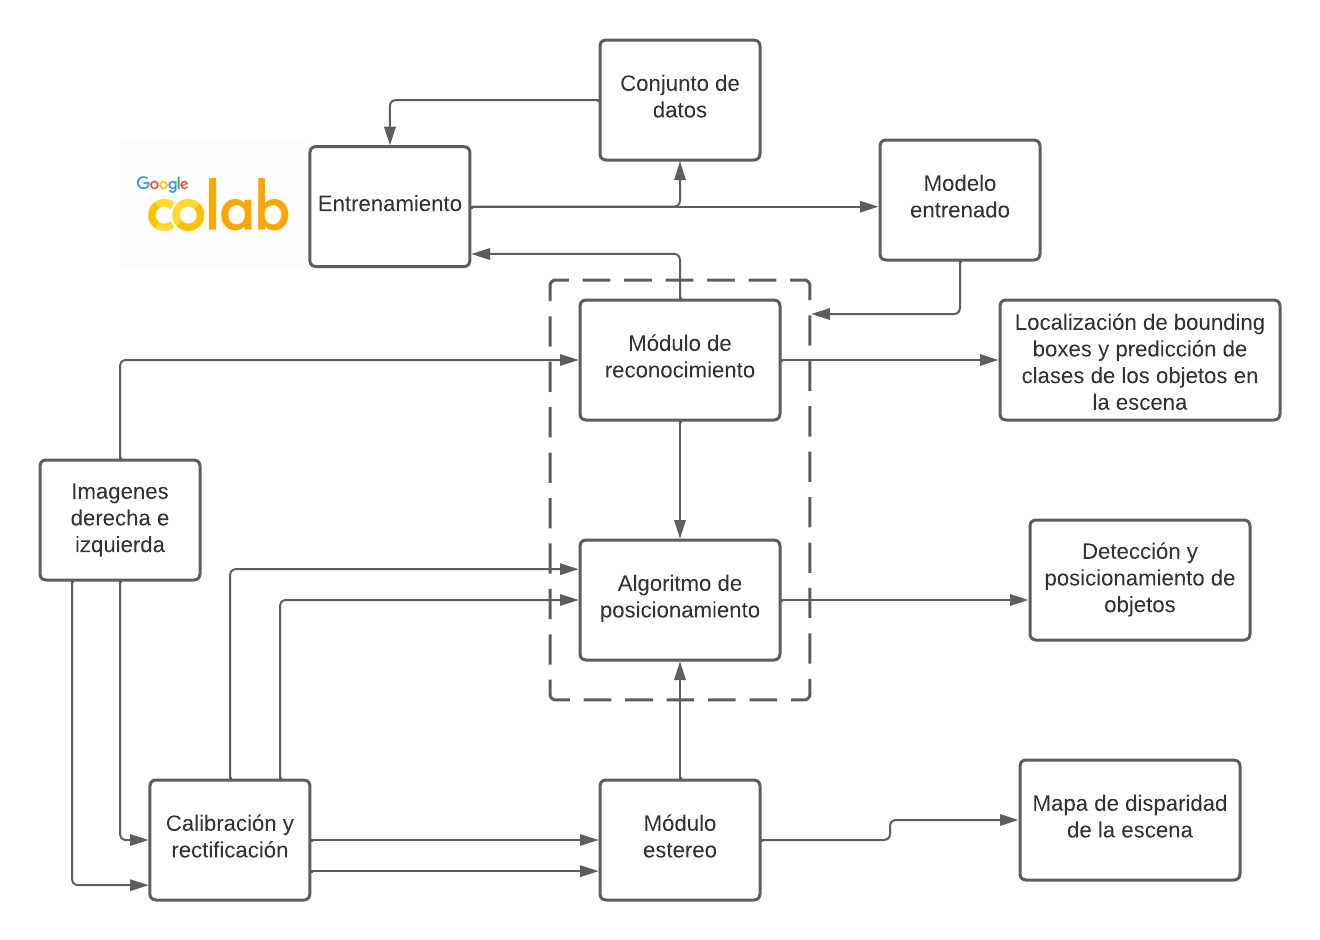
\includegraphics[scale=0.5]{Recursos/modos_func_paquete.png}
    \caption[Diagrama macro de la estructura del paquete.]{Diagrama macro de la estructura del paquete. {\footnotesize Fuente: El autor}}
    \label{modos_func_paquete}
\end{figure}
\section{Entorno de desarrollo}
\subsection{Servidor de Google Colaboratory}
Dado que el computador empleado en la programación del paquete cuenta con una gráfica integrada de recursos insuficientes para el entrenamiento de redes neuronales, se optó por usar los servidores de Google Colaboratory o Colab, este no es más que un producto gratuito de Google Research que permite a cualquier usuario escribir y ejecutar código de \textit{python} en el navegador, esta herramienta es un servicio de \textit{notebook} alojado en Jupyter (aplicación web interactiva para desarrollar software de código abierto) que no requiere configuración previa para usarlo y brinda acceso gratuito a recursos computacionales (GPU y RAM); sin embargo, en el caso de la red entrenada se empleó la versión de pago ``Google colab Pro'' para así tener acceso a una mejor tarjeta gráfica, mayor espacio de almacenamiento, de tal forma que se pudiesen contener conjuntos de datos más extensos (conjunto de datos de COCO) que con los recursos propios de la versión normal de Colab no sería posible.  Además, cuenta con una tarjeta RAM de alta velocidad y eliminar la limitación de tiempo de uso de 12 horas que posee la versión gratuita. Entre las características más importantes de Colab se tiene que:
\begin{itemize}
    \item En Colab los \textit{notebooks} se almacenan en Google drive, pero también pueden ser cargados desde Github, además de poder ser compartidos a cualquier usuario. Aunque esta comunicación no se limita a \textit{notebooks}, puesto que es posible montar el sistema de archivo de Google drive en un \textit{notebook} de Colab. Utilizando esta capacidad se guardó el paquete en Google drive y en Colab se procedió a entrenar importando los módulos necesarios, además de que los puntos de guardado y archivos generados en la rutina de entrenamiento se enviaban al almacenamiento de Google drive.
    \item El código es ejecutado en una máquina virtual (VM) exclusiva para la cuenta del usuario, la cuales se borran cuando están inactivas durante un tiempo prolongado o al superar un límite de tiempo de ejecución de 12 horas, este límite de tiempo fue una de las razones por las que se optó por la subscripción paga, ya que; la red requería un mayor tiempo para el entrenamiento.
    \item La cantidad de memoria de la máquina virtual en la versión Pro era de 166.83 GB para el almacenamiento y 25.46 GB de RAM, con estas capacidades fue posible experimentar con el conjunto de datos PASCAL VOC sin problema alguno, puesto que la versión gratuita tendía a alcanzar el límite de memoria con facilidad.
    \item Actualmente cuenta con 4 tipos de GPU que pertenecen a NVIDIA de la serie Tesla la K80, T4, P4 y P100. Aunque no hay una forma de elegir el tipo de GPU a la que se puede conectar el \textit{notebook} de Colab, todas las opciones disponibles cumplen con las especificaciones suficientes para entrenar modelos de reconocimiento, en el caso de este desarrollo se usó el P100.
\end{itemize}
\subsection{Editor de texto}
Se seleccionó como interfaz de desarrollo, al editor desarrollado y mantenido por Microsoft ``Visual Studio Code'', ya que este posee las siguientes cualidades:
\begin{itemize}
    \item Alternar entre intérpretes de \textit{Python}, versiones y entornos personalizados, el paquete fue desarrollado en la versión 3.8 de \textit{Python}.
    \item Ejecutar archivos de \textit{python} en un terminal de comandos integrado a la interfaz.
    \item La capacidad de configurar y ejecutar pruebas unitarias mediante unos pocos clics.
    \item Es un entorno ligero, ya que los recursos computacionales mínimos son: un procesador de 1.6 GHz, 2 GB de RAM en una arquitectura de 64 bits y 800 MB de espacio disponible en el disco duro.
    \item Una comunidad activa que actualiza y crea nuevas extensiones que mejoran la experiencia del editor.
    \item El soporte continuo de Microsoft y que a pesar de pertenecer a la empresa es una herramienta \textit{open source}.
    \item La facultad de configurar un \textit{Linter} que permita detectar el código sospechoso que no cumpla con un formato impuesto o uno personalizado. 
    \item La herramienta IntelliSense cuyas funciones principales son el auto completado y la desambiguación de nombres de variables, funciones y métodos.
\end{itemize}
\section{Estructura del paquete y sus dependencias}
Como se pudo ver en el capítulo II un paquete requiere más que solo el código utilizable para el usuario, si se quiere distribuir en el \textit{Python Package Index} (PyPI). Por este motivo se estructuró el directorio que contiene al paquete como en la Figura \ref{directorioCompletoPaquete}. 
\begin{figure}[H]
    \centering
    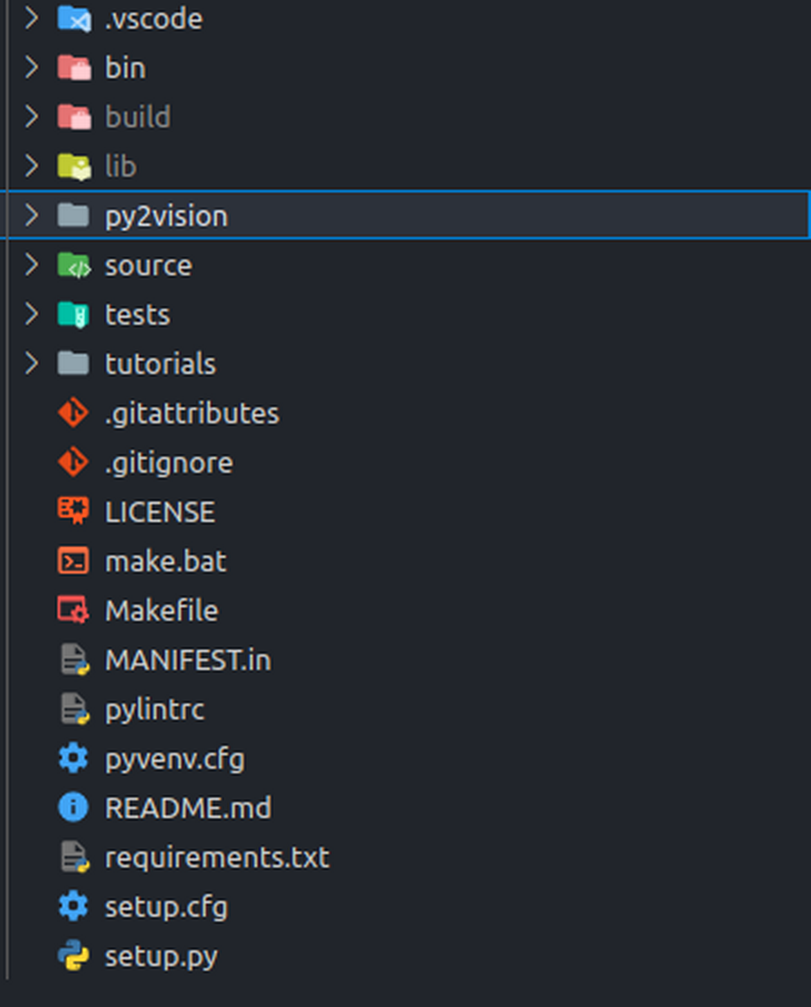
\includegraphics[scale=0.3]{Recursos/directoriosPaqueteNivelRoot.png}
    \caption[Directorio raíz del proyecto.]{Directorio raíz del proyecto. {\footnotesize Fuente: El Autor}}
    \label{directorioCompletoPaquete}
\end{figure}
A continuación se explicará la función de las carpetas y archivos presentes en la Figura \ref{directorioCompletoPaquete}:
\begin{itemize}
    \item \textbf{.vscode:} contiene el archivo json de configuración, generado por el editor de código, el cual le dice al mismo, ciertos ajustes del usuario, tales como: el uso de un \textit{Linter}, la ubicación del archivo que indica la configuración del \textit{Linter}, la ubicación o la ruta de la versión de \textit{Python}, la localización de los test unitarios e incluso el nombre que deben tener los archivos para considerarse test y poder ejecutarlos mediante el editor, en el caso de este paquete son test aquellos archivos cuyo nombre comience por ``test\_''.
    \item \textbf{bin y pyenv.cfg:} bin es una carpeta generada por pyenv, esta es una herramienta empleada para instalar diferentes versiones de \textit{Python} y cambiar entre ellas según los requerimientos del proyecto en el que se esté trabajando, esto implica que con pyenv es posible crear entornos virtuales que contengan un conjunto de paquetes instalados por el usuario, sin afectar a los paquetes instalados en otros proyectos. Por otro lado, pyenv.cfg es el archivo de configuración que tomara en cuenta la herramienta del mismo nombre al momento de generar la carpeta bin. 
    \\
    \\
    Para activar el entorno virtual es necesario utilizar el siguiente comando en la terminal desde la raíz del proyecto: 
    \begin{verbatim}
        source bin/activate
    \end{verbatim}
    El comando \textit{source} lee y ejecuta comandos del archivo especificado como argumento en el entorno de \textit{shell} actual.
    \item \textbf{Makefile, build, source y make.bat:} los dos archivos (Makefile y make.bat) dictan la configuración de la herramienta de documentación \textbf{Sphinx}, la cual puede ser ocupada mediante comandos en la terminal. La carpeta \textit{build} contiene todas las dependencias configuradas por Sphinx y la carpeta \textit{source} contiene la estructura de la documentación que puede ser mostrada en distintos formatos, en este caso se eligió un formato html, para que cualquier usuario con un navegador pueda conocer el funcionamiento del paquete.
    \item \textbf{py2vision:} es el nombre del paquete, por lo que esta carpeta contiene los módulos y submódulos de todo el paquete.
    \item \textbf{tests:} contiene los test unitarios aplicados a los módulos y submódulos que se encuentran en la carpeta py2vision.
   \item \textbf{tutorials:} En esta carpeta se encuentran 3 \textit{notebooks} de Jupyter los cuales pueden ser abiertos con Google Colab y en su interior se encuentran varias lecciones que ejemplifican el uso del paquete. Además alberga un script ejecutable llamado ``stereo\_tuner.py'' que construye una interfaz para ajustar los parámetros del algoritmo de correspondencia empleado en el paquete y un fichero ejecutable llamado get\_anchors\_k\_means.py que permite generar las dimensiones de los \textit{anchor boxes} utilizados en la detección de objetos analizando la estructura del conjunto de datos mediante el algoritmo de clusterización ``K means''.
    \item \textbf{MANIFEST.in:} cuando se construye el código que será distribuido, Python toma por defecto la carpeta del proyecto; sin embargo, hay algunos archivos que no deben dejarse por fuera, como puede ser el caso del setup.py, README.txt, pyproject.toml y setup.cfg. Para estos casos es que existe el archivo MANIFEST.in, ya que este incluye o excluye los archivos que deben o no deben ser distribuidos.
    \item \textbf{pylintrc:} contiene la configuración del formato que sigue el paquete, en el caso de py2vision se sigue el estilo de Google, el cual puede observarse al detalle en https://google.github.io/styleguide/pyguide.html.
    \item \textbf{setup.cfg:} Como se pudo ver en la Figura \ref{estructuraSetupTools} es un archivo necesario en caso de utilizar Setuptools para la distribución.
    \item \textbf{setup.py:} Es el archivo de configuración en caso de usar Distutils para la distribución, se dejaron ambas opciones de ser necesario uno u otro.
    \item \textbf{requirements.txt:} Es un archivo de texto que contiene los paquetes externos que necesita py2vision para funcionar.
\end{itemize}
\section{Diseño de la arquitectura del paquete}
El paquete ''py2vision'' se encuentra diseñado sobre el lenguaje de programación \textit{python} y utiliza las siguientes dependencias externas para agilizar y optimizar el desarrollo:
\begin{itemize}
    \item Numpy y pandas: para el manejo algebraico y presentación de los datos.
    \item Opencv-contrib-python: se usa para recibir la entrada de datos y exportar en formatos de vídeo o imagen según sea el caso, así como también para la calibración de las cámaras y realizar el mecanismo estéreo, si el usuario tiene instalada la versión base de este paquete se recomienda desinstalarla e instalar esta, para no ocasionar conflictos de dependencias.
    \item Tensorflow/keras: como \textit{framework} de \textit{machine learning}.
    \item wget: se usa cuando es necesario descargar contenido de internet, en esta ocasión se usó para poder descargar archivos que contengan los pesos de una red y así aplicar transferencia de aprendizaje o simplemente recuperar los pesos de la red original empleada.
    \item pyyaml y h5py: ambos son necesarios al entrenar para recuperar los pesos a partir de un punto de guardado.
\end{itemize}
Al adentrarnos en el directorio de py2vision podemos observar la siguiente distribución de carpetas:
\begin{figure}[H]
    \centering
    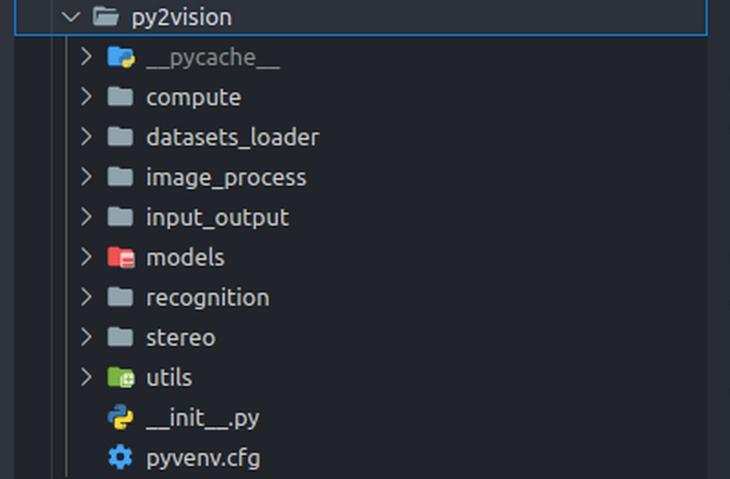
\includegraphics[scale=0.4]{Recursos/pytwovision_folder.jpg}
    \caption[Distribución de la carpeta del proyecto.]{Distribución de la carpeta del proyecto. {\footnotesize Fuente: El Autor}}
    \label{pytwovision_folder}
\end{figure}
En la Figura \ref{dependency_modules} se puede observar un diagrama que resalta las dependencias existentes en el paquete py2vision. 
\begin{figure}[H]
    \centering
    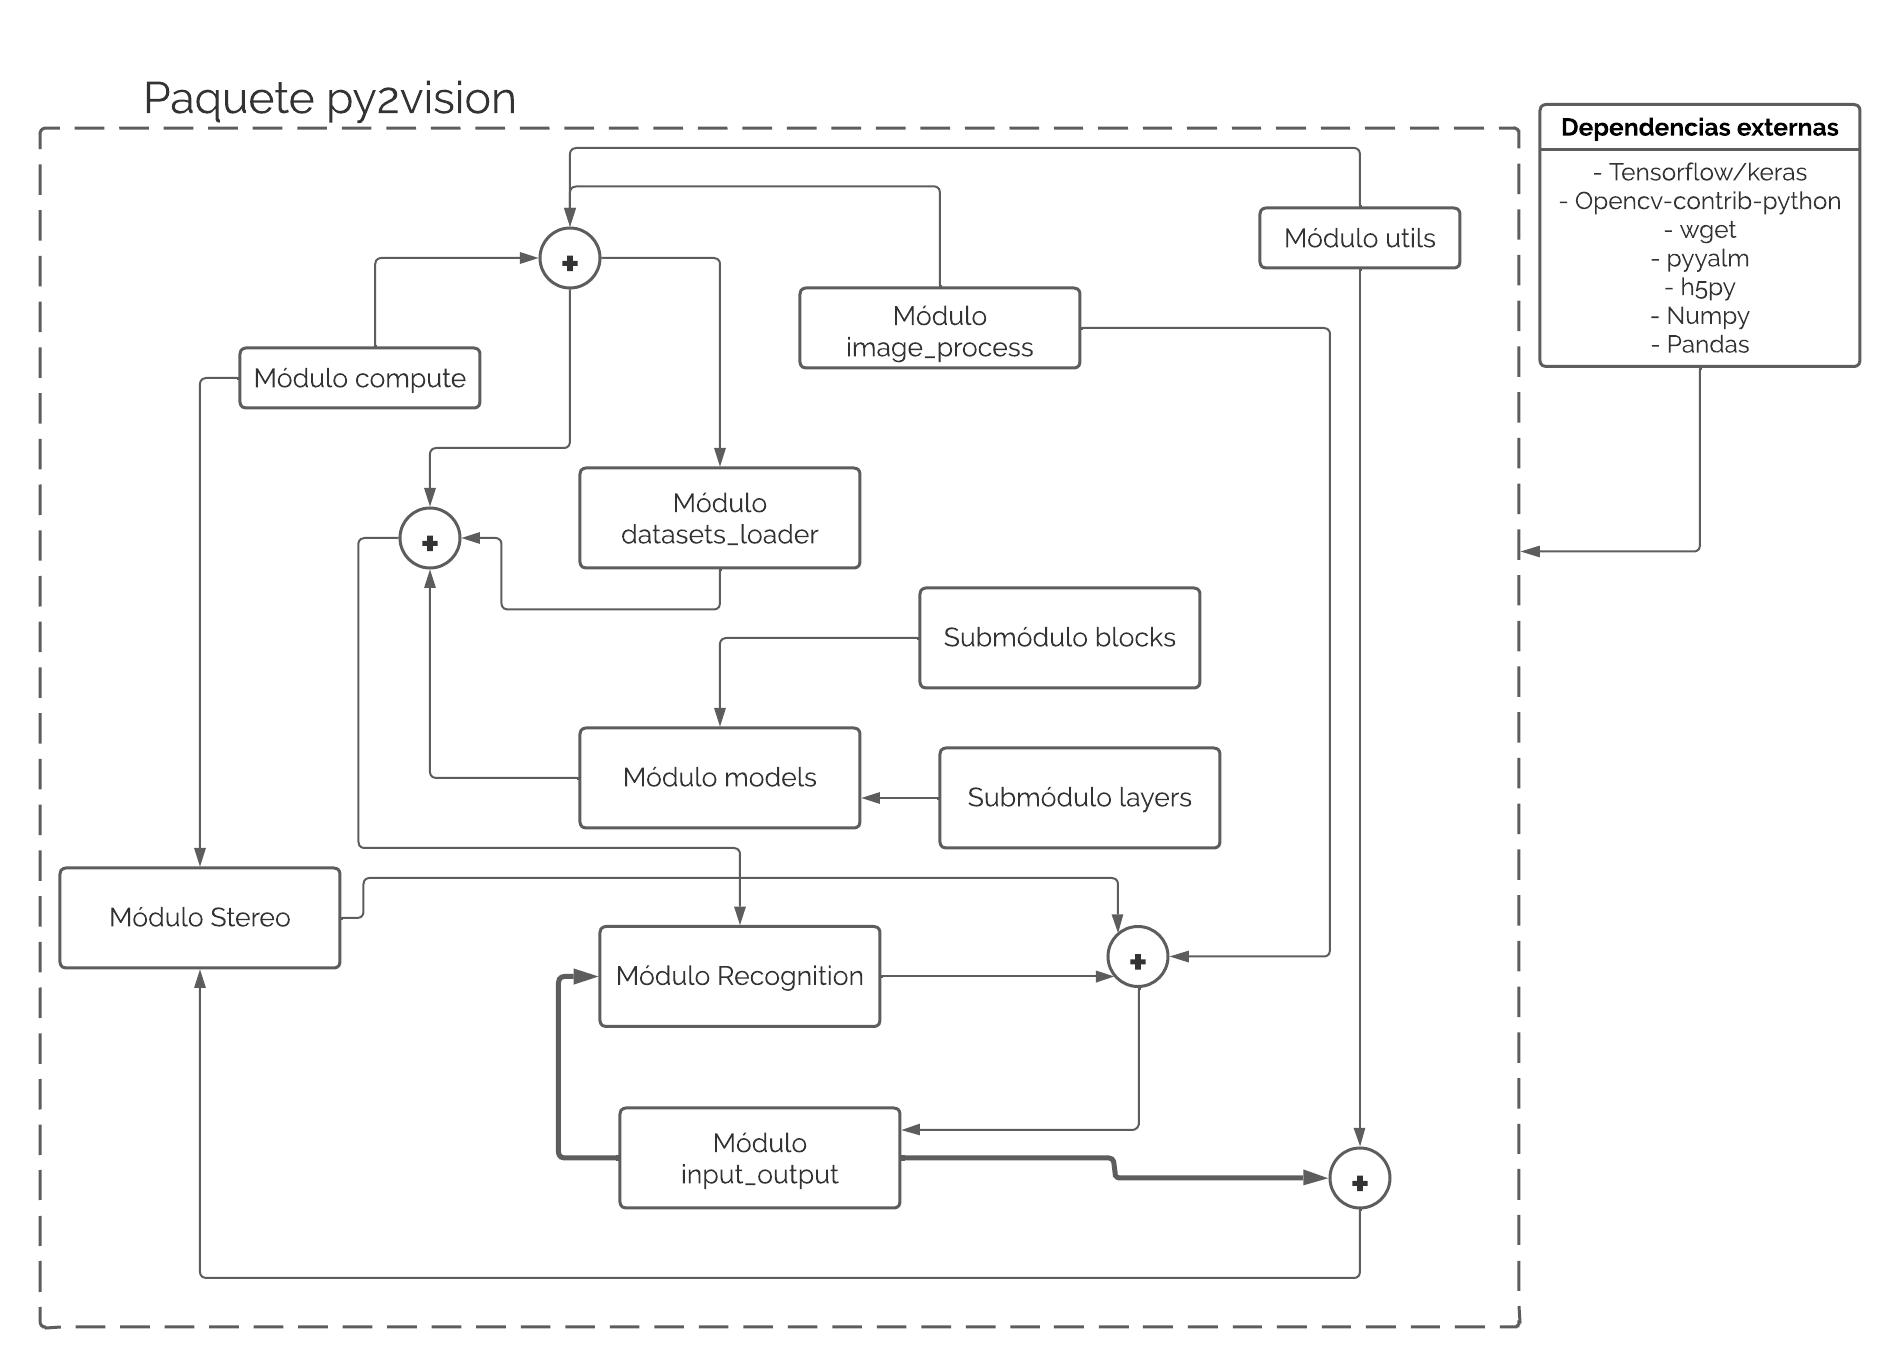
\includegraphics[scale=0.5]{Recursos/diagrama_dependencias.png}
    \caption[Diagrama de dependencias de py2vision.]{Diagrama de dependencias de py2vision. {\footnotesize Fuente: El Autor}}
    \label{dependency_modules}
\end{figure}
Como se pudo observar en la Figura \ref{pytwovision_folder} cada carpeta o módulo cumple el rol que indica su nombre, sin embargo en breve se explicara a detalle la distribución de clases y métodos, así como también los patrones de diseño y sus funciones.
\subsection{Módulo compute}
Este directorio se creó con el fin de albergar los cálculos que puedan necesitar los mecanismos estéreo y los requeridos por las redes neuronales. Cuenta con los archivos:
\begin{itemize}
    \item \textbf{error\_compute.py}: actualmente cuenta con un solo método llamado \\``re\_projection\_error'', el cual calcula la distancia de la imagen entre un punto proyectado y uno medido, es utilizado para hallar el error de calibración de las cámaras.
    \item \textbf{yolov3\_calculus.py:} contiene la clase \textbf{YoloV3Calculus} que se encarga de agregar la capa de predicción en una red YOLO versión 3, convertir las matrices que contengan las coordenadas de \textit{bounding boxes} de un formato ($xmin$, $ymin$, $xmax$, $ymax$) a un formato ($cx$, $cy$, $w$, $h$) donde $cx$ y $cy$ son las coordenadas del punto central del \textit{bounding box} y las variables $w$ y $h$ son el ancho y el alto del cuadro respectivamente, dicha conversión puede hacerse en ambos sentidos.
    \\
    \\
    También se encarga de calcular el valor del IoU y aplicar el algoritmo de \textit{Non maximum suppression} (Ver Apéndice \ref{CAP:anexo2}) para filtrar los \textit{bounding boxes} que no cumplan con cierto umbral, con el fin de obtener predicciones con una menor cantidad de ruido y calcular el error de la red.
\end{itemize}
\subsection{Módulo datasets\_loader}
Se elaboró debido a que la forma en que se presentan los conjuntos de datos introducidos en una red puede variar dependiendo del tipo de reconocimiento (sea detección, clasificación o segmentación) e incluso el mecanismo de entrenamiento de cada arquitectura de red varia, en ocasiones requiere un preprocesamiento especial. Por estos motivos en este módulo cada archivo debe contener una clase que adapte el conjunto de datos para poder ser introducido en una red neuronal. Actualmente alberga la clase \textbf{YoloV3DatasetGenerator}, la cual toma las anotaciones de un archivo que contenga las localizaciones de las imágenes del conjunto, sus \textit{bounding boxes} y la clase a la que pertenece el objeto y las adapta a la red para su entrenamiento y evaluación.  
\subsection{Módulo image\_process}
El concepto de este módulo se basa en poder aplicar diferentes efectos a imágenes de entrada utilizando una clase en común y de ser necesario apilar un efecto sobre otro a dicha imagen. Debido a esto todo el módulo se aprovecha del patrón de diseño de software conocido como \textit{Decorator} el cual permite:
\begin{itemize}
    \item Extraer el comportamiento de un objeto sin crear una nueva subclase.
    \item Combinar varios comportamientos envolviendo un objeto con varios decoradores.
    \item Cada clase tiene una sola responsabilidad, lo que hace posible dividir una clase monolítica que implementa muchas variantes posibles de comportamiento, en varias clases más pequeñas, de modo que facilita el agregar un nuevo procesamiento en la imagen.
\end{itemize}
Este directorio se encuentra estructurado de la siguiente manera:
\begin{figure}[H]
    \centering
    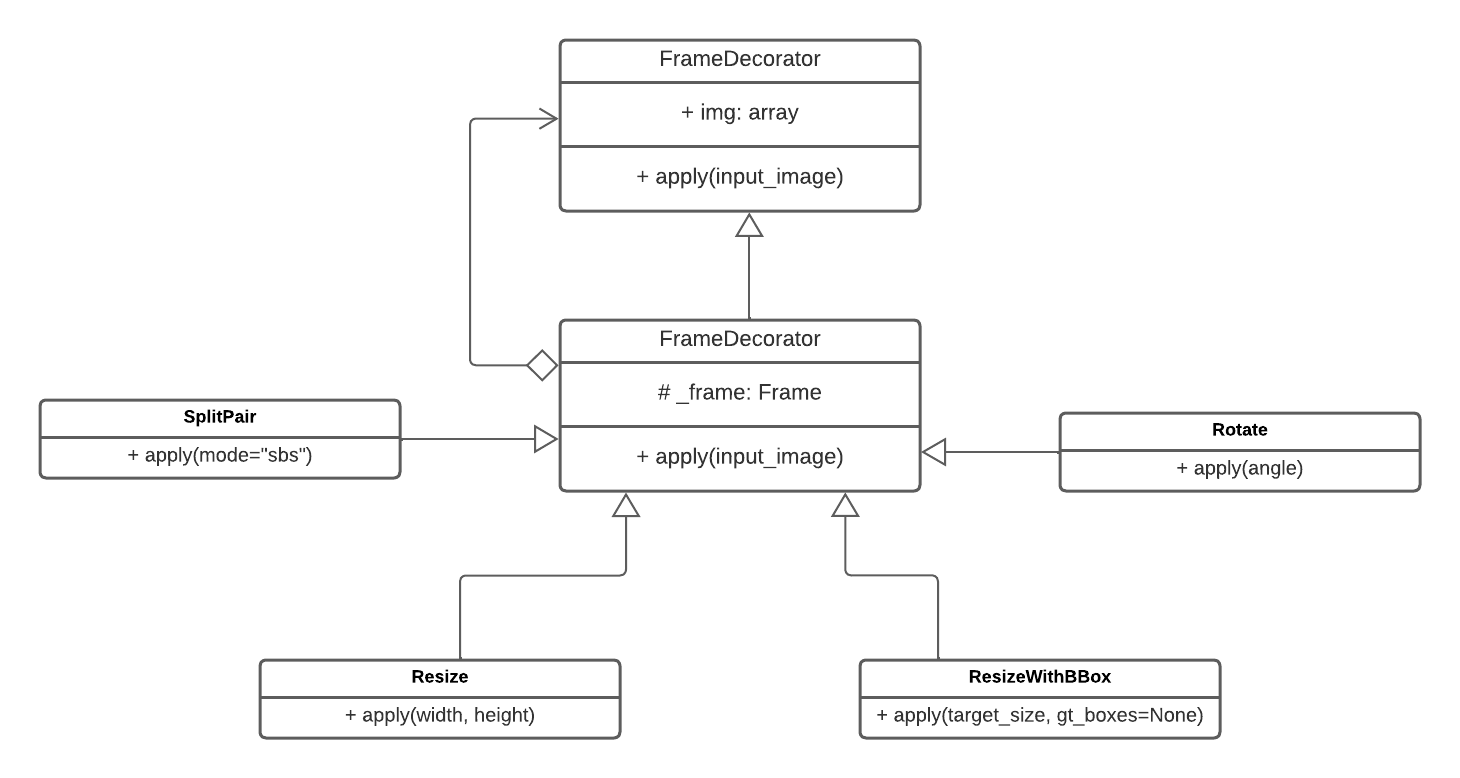
\includegraphics[scale=0.4]{Recursos/image_process_uml.png}
    \caption[Diagrama de clases UML: Módulo image\_process.]{Diagrama de clases UML: Módulo image\_process. {\footnotesize Fuente: El Autor}}
    \label{image_process_uml}
\end{figure}
En la Figura \ref{image_process_uml} se puede observar un diagrama que representa las relaciones entre las clases del módulo, los atributos de cada clase ubicados en la sección media de los rectángulos y sus correspondientes métodos (la sección baja de los rectángulos). En este tipo de diagramas se tiene por convención que el símbolo ``+'' indica que un atributo o un método es público, es decir; que desde una clase externa que no herede de la clase anfitriona es posible acceder a dicha variable, mientras que el símbolo ``\#'' indica que es protegida, por lo que subclases que heredan de la clase padre pueden acceder a la variable, pero no es posible acceder a dicha variable desde clases o entornos externos, también existe el símbolo ``-'' implica que la variable es privada por lo que solo es posible acceder a ella desde la clase anfitriona.
\\
\\
Además en dicho diagrama (Ver Figura \ref{image_process_uml}) se puede observar que la clase \textbf{FrameDecorator} hereda de la clase \textbf{Frame} y a su vez tiene una relación de agregación, esto significa que aunque no exista la clase \textbf{FrameDecorator} la clase \textbf{Frame} todavía tiene motivos para existir, ya que podría tener otro decorador base que dependa de ella, el resto de las clases heredan de \textbf{FrameDecorator} y son precisamente los distintos decoradores que aplican los efectos en la imagen de entrada.
\subsection{Módulo utils}
En su interior se encuentran todas aquellas funcionalidades que no encajan en el resto de los módulos, tales como:
\begin{itemize}
    \item \textbf{annotations\_parser.py}: este archivo está basado en el patrón de diseño \textit{visitor}, debido a que se necesitaba que el software pudiese convertir anotaciones que se encontraran en diferentes formatos (bien sea JSON, XML, txt, etc.) a anotaciones compatibles con los generadores de conjuntos de datos dentro del módulo datasets\_loader. \textit{Visitor} es un patrón cuya función es separar algoritmos de los objetos sobre los que operan, ofreciendo así las siguientes ventajas:
    \begin{itemize}
        \item Es posible introducir un nuevo comportamiento que puede funcionar con objetos de clases diferentes sin cambiar esas clases.
        \item Puedes tomar varias versiones del mismo comportamiento y ponerlas en la misma clase.
        \item Un objeto visitante puede acumular cierta información útil mientras trabaja con varios objetos. Esto puede resultar útil cuando quieras atravesar una compleja estructura de objetos, como un árbol de objetos, y aplicar el visitante a cada objeto de esa estructura.
    \end{itemize}
    En la Figura \ref{annotations_parser_uml} se puede apreciar que la interfaz Parser tiene una relación de composición con la interfaz visitante (\textbf{AnnotationsFormat}), lo que implica que \textbf{Parser} necesita de la clase visitante para funcionar. \textbf{YoloV3AnnotationsFormat} implementa el formato de anotaciones compatible con la red del mismo nombre, mientras que \textbf{XmlParser} al heredar de la clase Parser redirige la llamada al método adecuado del visitante correspondiente, en este caso este sería el método visit\_xml\_parser(). 
    \begin{figure}[H]
        \centering
        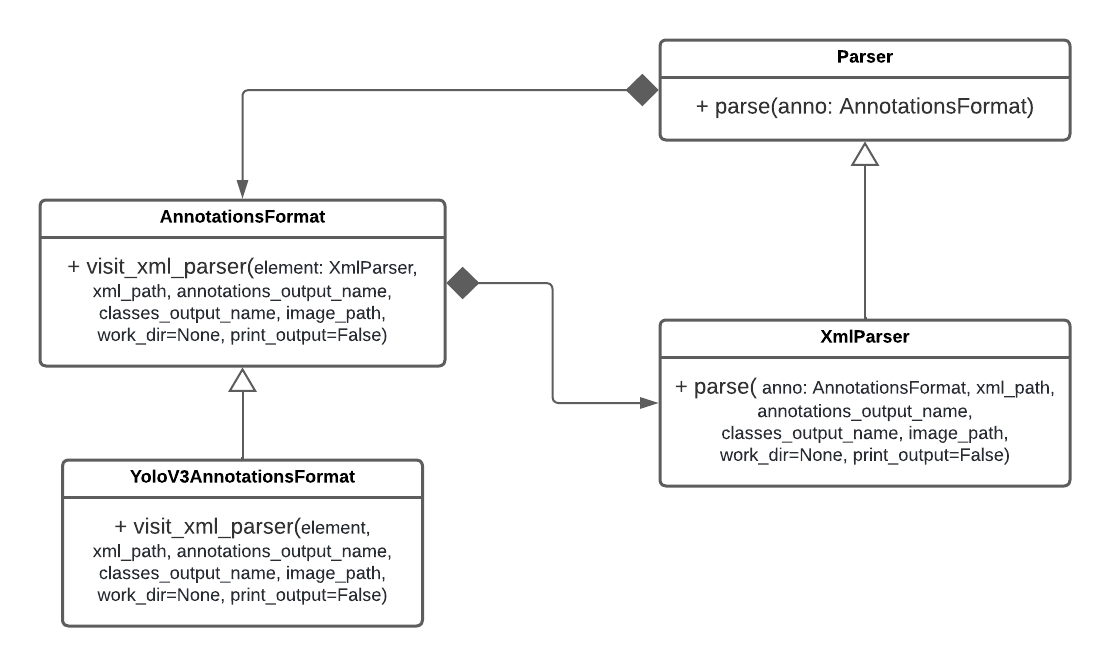
\includegraphics[scale=0.5]{Recursos/annotations_parser_uml.png}
        \caption[Diagrama de clases UML: annotations\_parser.]{Diagrama de clases UML: annotations\_parser. {\footnotesize Fuente: El Autor}}
        \label{annotations_parser_uml}
    \end{figure}
    \item \textbf{annotations\_helper.py:} contiene una clase llamada \textbf{AnnotationsHelper}, la cual recibe como entrada la localización de las anotaciones generadas por annotations\_parser.py y las convierte en variables del tipo \textbf{Dataframe} las cuales pueden ser manipuladas por la librería pandas, para luego separar el conjunto de datos en dos partes e incluso generar los archivos de anotaciones de cada una.
    \item \textbf{draw.py:} posee un método que dibuja las líneas epipolares captadas a partir de dos imágenes y otro que traza los \textit{bounding boxes} en una imagen.
    \item \textbf{gen\_pattern.py:} crea un archivo svg con el patrón de calibración estéreo, ya sea; un patrón de cuadros de ajedrez o un patrón en forma de círculos.
    \item \textbf{label\_utils.py:} alberga métodos que contribuyen con el funcionamiento de los generadores de conjuntos de datos en datasets\_loader.
\end{itemize}
\subsection{Módulo models}
Se ocupa de generar las capas y bloques que conforman las arquitecturas de las diferentes redes neuronales utilizando las herramientas que ofrece Tensorflow. Dentro de models hay dos submódulos blocks y layers, el primero almacena agrupaciones de capas, las cuales pueden ser propias de Tensorflow o capas personalizadas las cuales se encuentran en el submódulo layers. 
\\
\\
En este módulo hay dos patrones de diseño el primero está en el submódulo blocks en el archivo backbone\_block.py, este emplea el patrón \textit{Strategy} para separar los algoritmos de arquitecturas de red conocidas como \textit{backbones networks}, las cuales son redes que fungen como extractores de \textit{features} sobre sus datos de entrada. Este patrón da las siguientes ventajas:
\begin{itemize}
    \item Separa los detalles de implementación de un algoritmo del código que lo utiliza.
    \item Sustituye la herencia por composición.
    \item Se pueden introducir nuevas estrategias sin tener que cambiar el contexto, que en este caso es la clase \textbf{BackboneBlock} de la Figura \ref{backbone_block_uml}.
\end{itemize}
\begin{figure}[H]
    \centering
    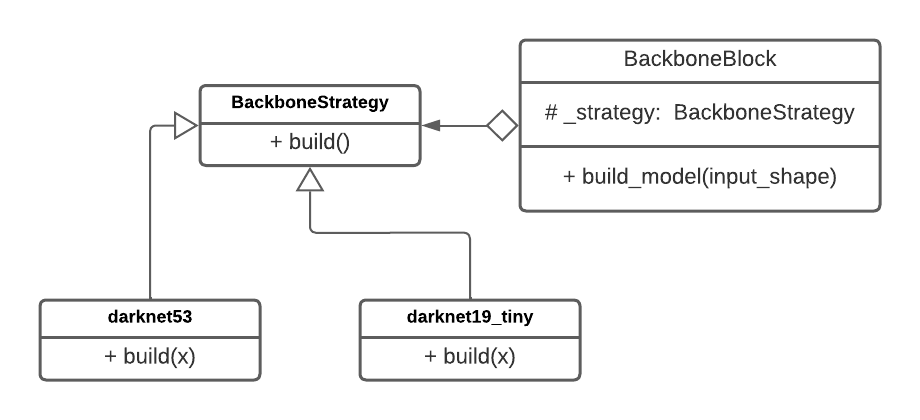
\includegraphics[scale=0.5]{Recursos/backbone_block_uml.png}
    \caption[Diagrama de clases UML: backbone\_block.]{Diagrama de clases UML: backbone\_block. {\footnotesize Fuente: El Autor}}
    \label{backbone_block_uml}
\end{figure}
Como se puede ver en la Figura \ref{backbone_block_uml} hay dos estrategias que heredan del contexto, sin embargo de ser necesario es posible implementar más con solo agregar la clase de la estrategia correspondiente.
\\
\\ 
Dado que la cantidad de arquitecturas de red existentes para realizar reconocimiento es enorme, se requería una forma de organizarlas sin generar dependencias caóticas entre objetos, por este motivo se empleó el segundo patrón de este módulo, el cual es conocido como \textit{Mediator} este restringe las comunicaciones directas entre objetos forzándolos a colaborar únicamente a través de un objeto mediador, el cual como se puede ver en la Figura \ref{models_manager_uml} se representa con la interfaz \textbf{ModelManagerInterface} y su mediador concreto es \textbf{ModelManager}, ya que este almacena todos los modelos de red programados en el software.
\begin{figure}[H]
    \centering
    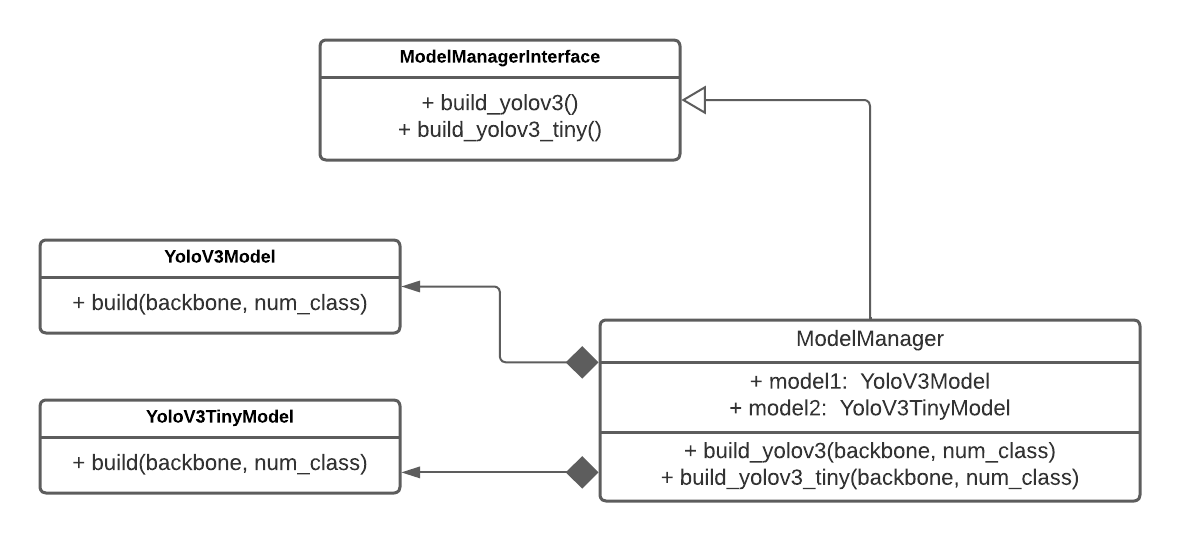
\includegraphics[scale=0.5]{Recursos/Model_Manager_uml.png}
    \caption[Diagrama de clases UML: models\_manager.]{Diagrama de clases UML: models\_manager. {\footnotesize Fuente: El Autor}}
    \label{models_manager_uml}
\end{figure}
\subsection{Módulo recognition}
Utiliza el patrón \textit{Bridge} para separar la abstracción usada por el usuario, del flujo de trabajo de una red neuronal que engloba el entrenamiento, inferencia, imprimir la estructura de la red, evaluarla y recuperar los pesos pre-entrenados (ver Figura \ref{bridge_uml}).
\begin{figure}[H]
     \centering
     \begin{subfigure}[b]{0.4\textwidth}
        \centering
        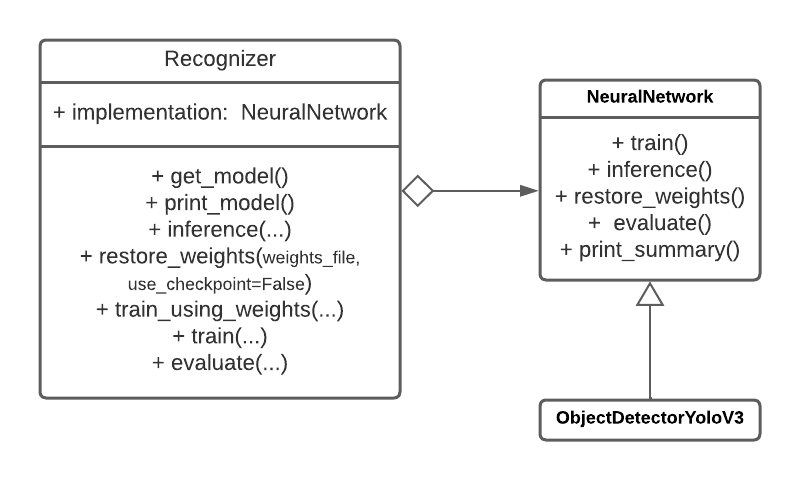
\includegraphics[scale=0.33]{Recursos/bridge_uml.png}
        \caption[Patrón \textit{bridge} en archivo selector.]{Patrón \textit{bridge} en archivo selector. {\footnotesize Fuente: El Autor}}
        \label{bridge_uml}
     \end{subfigure}
     \hspace{0.05em}
     \begin{subfigure}[b]{0.4\textwidth}
         \centering
        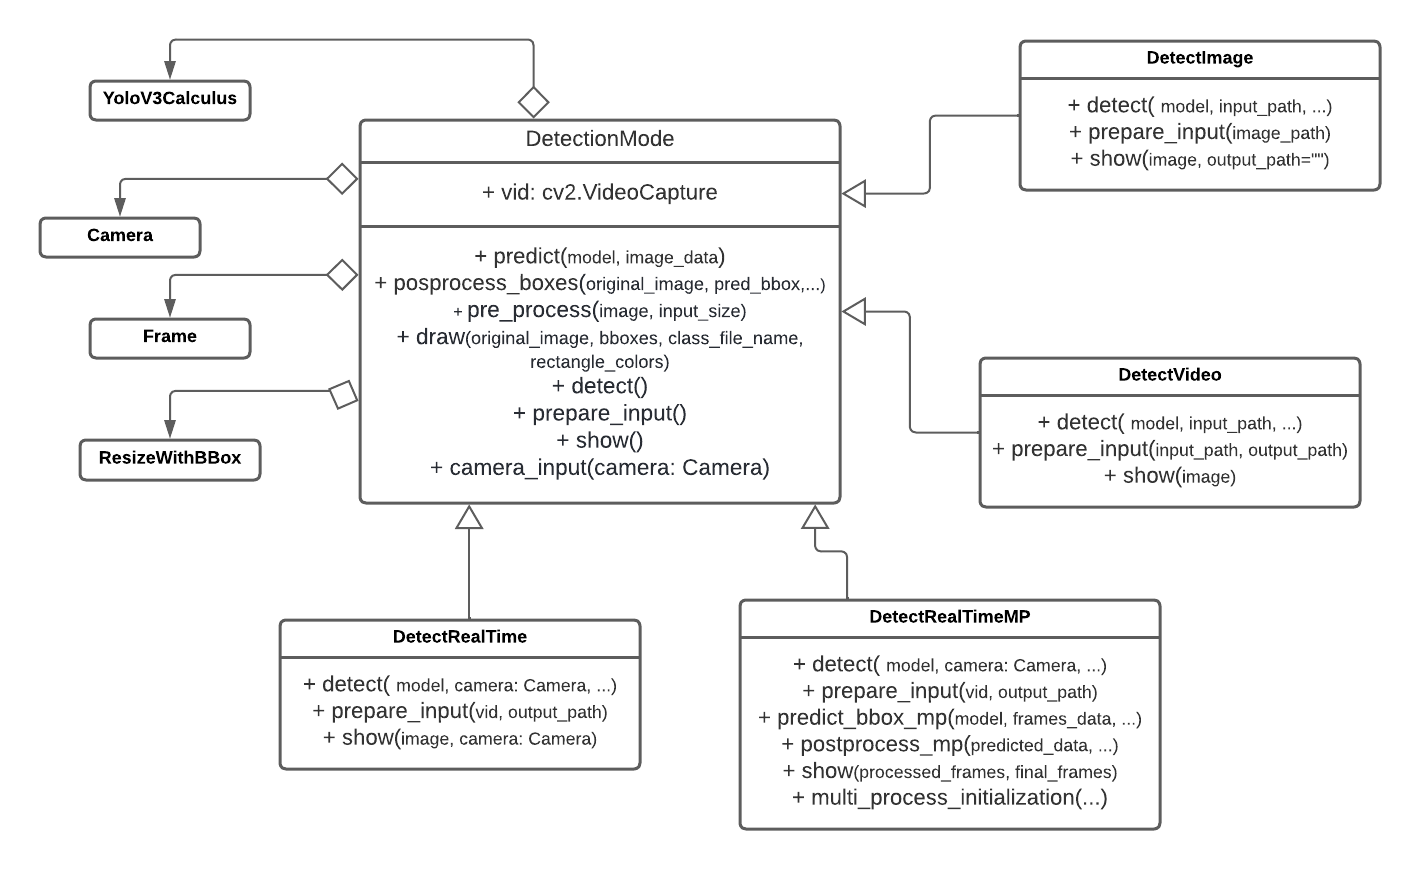
\includegraphics[scale=0.33]{Recursos/template_method_uml.png}
        \caption[Patrón \textit{template method} en archivo detection\_mode.]{Patrón \textit{template method} en archivo detection\_mode. {\footnotesize Fuente: El Autor}}
        \label{template_method_uml}
     \end{subfigure}
     \hspace{1em}
\caption{Diagramas de clases UML: Módulo recognition}
\label{recognition_umls}
\end{figure}
También en el archivo detection\_mode se aplicó el patrón \textit{Template method} de la Figura \ref{template_method_uml}, dado que; este fichero contiene 4 formas de inferencia: a tiempo real, utilizando multiprocesamiento, cuando la entrada es un archivo mp4 y cuando la entrada es una imagen. Sin embargo estas 4 formas comparten algunos procesos en común y su estructura es similar, por esto para poder maximizar la reutilización de código se eligió dicho patrón, a la vez que permite separar en métodos cada etapa de la inferencia.
\subsection{Módulo stereo}
Este comprende el mecanismo estéreo del cual se hablara en el capítulo V. El primer patrón que ocupa es \textit{Strategy} para elegir la metodología de correspondencia, en la Figura \ref{strategy_matcher_uml} se puede observar que actualmente existe solo una estrategia (StereoSGBM), sin embargo el patrón es capaz de aceptar ``n'' metodologías de correspondencia. 
\begin{figure}[H]
    \centering
    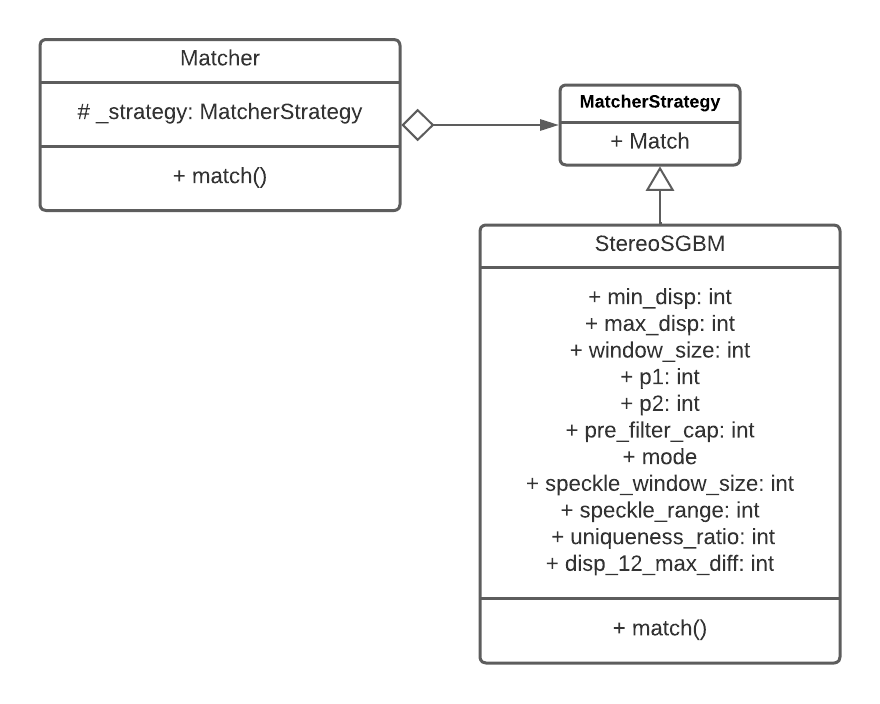
\includegraphics[scale=0.5]{Recursos/strategy_matcher_uml.png}
    \caption[Diagramas de clases UML: en fichero match\_method.]{Diagramas de clases UML: en fichero match\_method. {\footnotesize Fuente: El Autor}}
    \label{strategy_matcher_uml}
\end{figure}
El segundo patrón es ``Builder'' el cual se implementa en la Figura \ref{builder_stereo_uml}, en esta se aprecia que \textbf{StereoController} es la clase directora, la cual define el orden en el que se invocarán los pasos de construcción, por lo que puedes crear y reutilizar configuraciones específicas de los productos (\textbf{StandardStereo}). La interfaz constructora (\textbf{StereoSystemBuilder}) declara los pasos de construcción del producto que todos los tipos de objetos constructores tienen en común. El constructor concreto (\textbf{StandardStereoBuilder}) ofrece una implementación del mecanismo estéreo.
\begin{figure}[H]
    \centering
    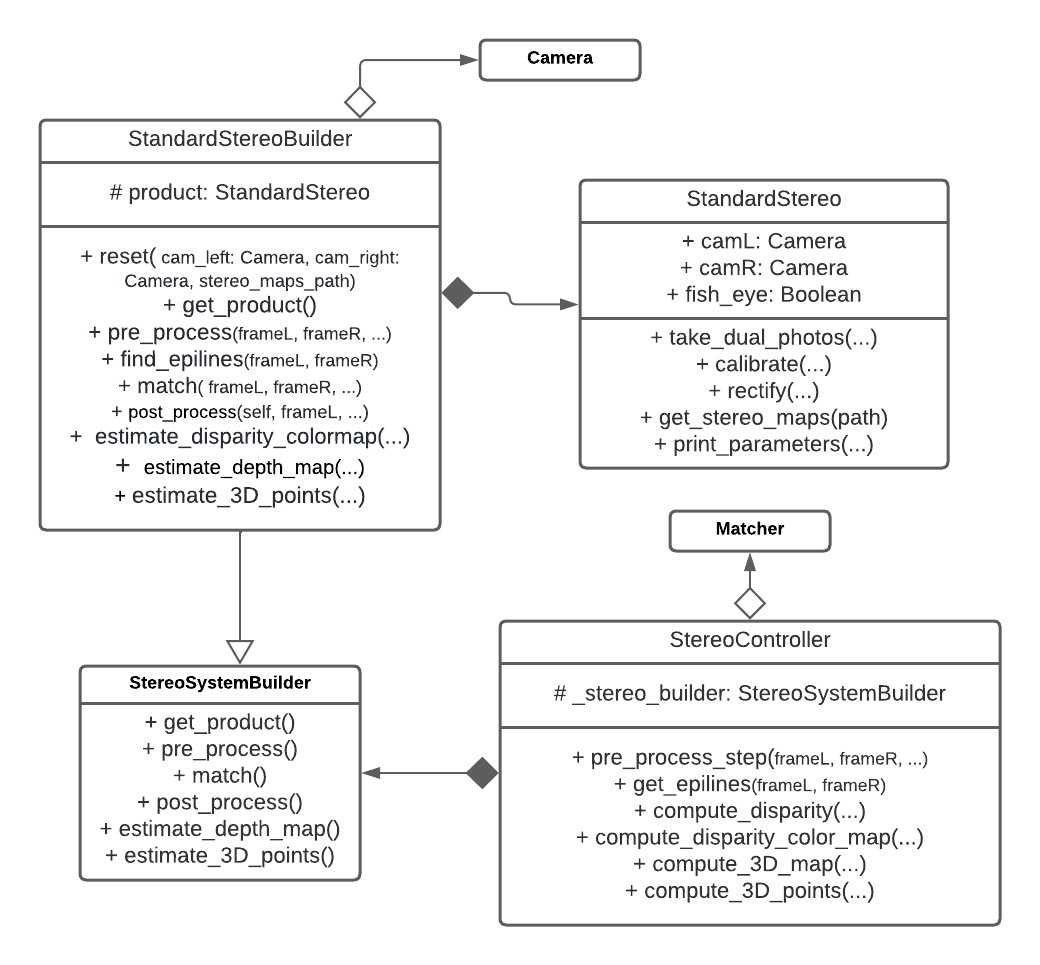
\includegraphics[scale=0.5]{Recursos/builder_uml.png}
    \caption[Diagrama de clases UML: mecanismo estéreo.]{Diagrama de clases UML: mecanismo estéreo. {\footnotesize Fuente: El Autor}}
    \label{builder_stereo_uml}
\end{figure}
\subsection{Módulo input\_output}
Se diseñó con el fin de contener las clases que permiten la entrada de datos al sistema estéreo y de reconocimiento a través de hardware externo bien sean cámaras, archivos de vídeo o incluso transmisión en vivo mediante wifi, además de obtener los parámetros intrínsecos e extrínsecos del medio físico que capturo las imágenes. Por otro lado, su otra función es fusionar las capacidades del módulo recognition y el módulo stereo en el archivo vision\_system.py que alberga la clase del mismo nombre, la cual ejecuta el algoritmo de posicionamiento cuando la entrada es vídeo o imágenes, de tal forma que se obtenga la salida correspondiente.%

%==================================================================
\chapter{DESCRIPCIÓN DEL ENTORNO DE TRABAJO DEL PAQUETE}\label{CAP:entorno}
%\markboth{Tu Segundo Capítulo}{Tu Segundo Capítulo}%
  En este capítulo se argumentará la elección de las partes del sistema de adquisición de datos, comparando el hardware seleccionado con las otras opciones evaluadas. También se ilustrarán las dimensiones físicas del soporte y las características de las cámaras empleadas en las pruebas realizadas al paquete.
\section{Características requeridas}
Para poder comprobar el correcto funcionamiento del software, el sistema físico como mínimo debía poseer las siguientes propiedades:
\begin{enumerate}
    \item Capacidad de procesamiento que permita ejecutar el algoritmo de reconocimiento y el de posicionamiento.
    \item Comunicación con el computador donde se desarrolló el paquete.
    \item Cámaras con características similares, preferiblemente iguales para poder realizar el posicionamiento correctamente.
    \item Facilidad de implementación. 
    \item Memoria suficiente que permita guardar el paquete junto a las librerías de las que depende para su funcionamiento.
    \item Una interfaz de usuario accesible.
\end{enumerate}
\section{Estrategias de adquisición de datos}
Se evaluaron 5 estrategias para poder probar las funcionalidades del software diseñado, con el fin de compararlas mediante un gráfico de araña respecto a las cualidades más importantes a tomar en cuenta. 
\\
En todas las estrategias hay una constante y ese es el computador empleado para el diseño del paquete el cual es una Laptop HP 15-dy2xxx con las siguientes especificaciones:
\begin{itemize}
    \item Procesador Quad-core i3-1115G4, con 3.00GHz.  
    \item 8 GB de memoria RAM.
    \item Tarjeta gráfica Intel UHD graphics.
    \item Almacenamiento SSD de 256 GB.
    \item Sistema operativo Linux con la distribución Ubuntu.
    \item Arquitectura de 64 bits.
\end{itemize}
\subsection{Estrategias con módulos StereoPi}
Se evaluaron 3 estrategias distintas que utilizan 3 versiones del módulo StereoPi, las versiones Slim y V1 con el procesador del Raspberry Pi compute module 3+ lite, mientras que la versión 2 del StereoPi con él compute module versión 4 lite. Él compute module actúa como un procesador mientras que el StereoPi funciona como interfaz que recibe las imágenes de las cámaras y se comunica con el computador o con el CM (Compute Module). De igual forma las versiones Slim y V1 se previó usarlas con las cámaras Raspberry Pi V1 (sensor OV5647) y la StereoPi V2 con el sensor IMX219, en la Figura \ref{estrategias_stereopi} se pueden observar el como se conectarían dichas configuraciones, así como también la dirección del flujo de datos.
\begin{figure}[H]
     \centering
     \begin{subfigure}[b]{0.4\textwidth}
        \centering
        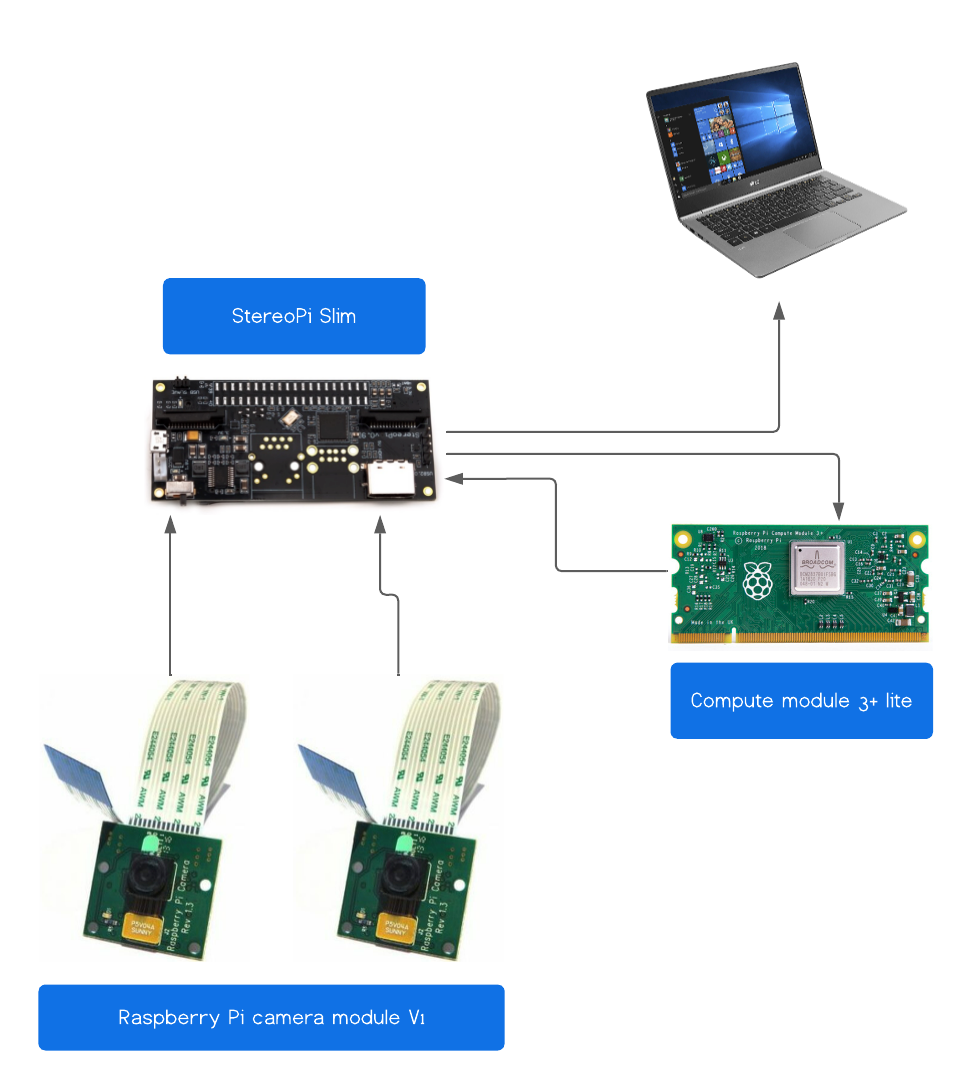
\includegraphics[scale=0.4]{Recursos/estrategia_stereopi_slim.png}
        \caption[Estrategia StereoPi Slim.]{Estrategia StereoPi Slim. {\footnotesize Fuente: El Autor}}
        \label{estrategia_slim}
     \end{subfigure}
     \hfill
     \begin{subfigure}[b]{0.4\textwidth}
         \centering
        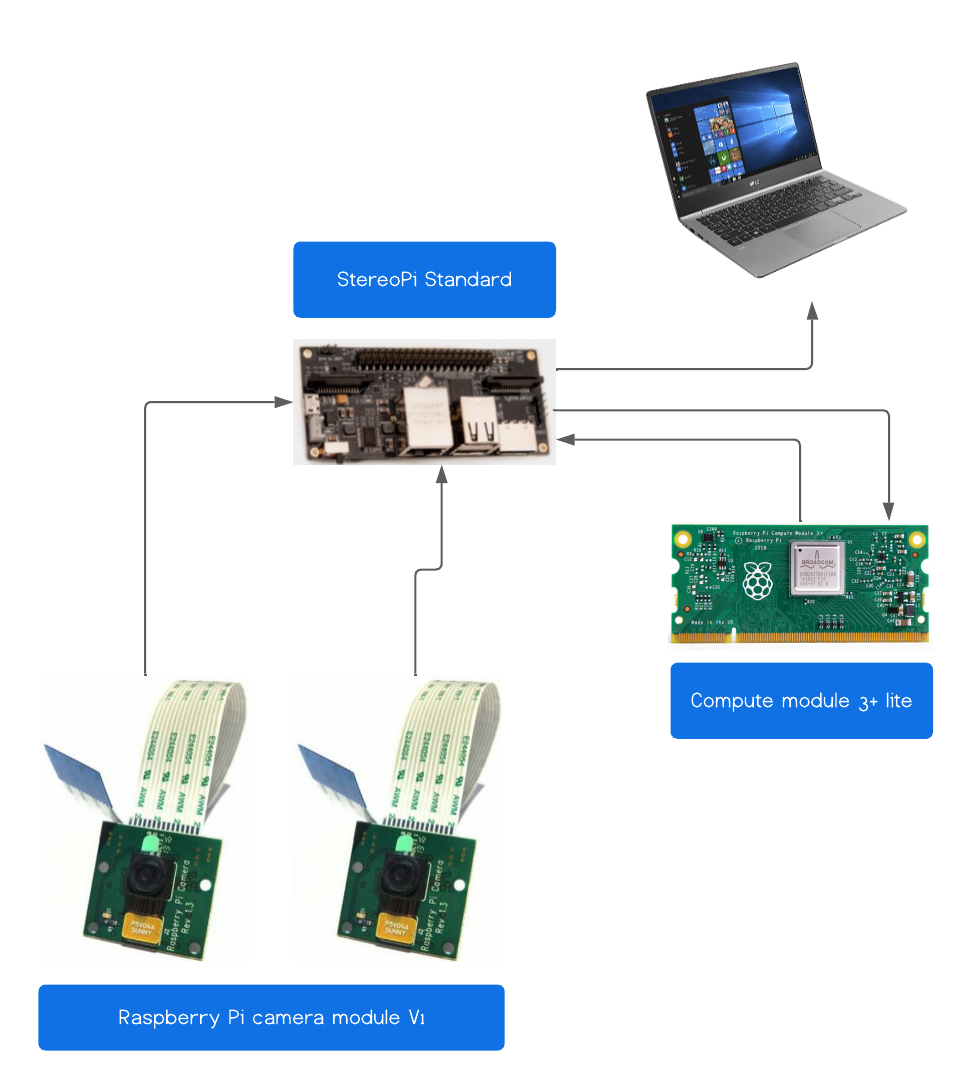
\includegraphics[scale=0.4]{Recursos/estrategia_stereo_pi_standard.png}
        \caption[Estrategia StereoPi V1.]{Estrategia StereoPi V1. {\footnotesize Fuente: El Autor}}
        \label{estrategia_v1}
     \end{subfigure}
     \hfill
     \begin{subfigure}[b]{0.4\textwidth}
         \centering
        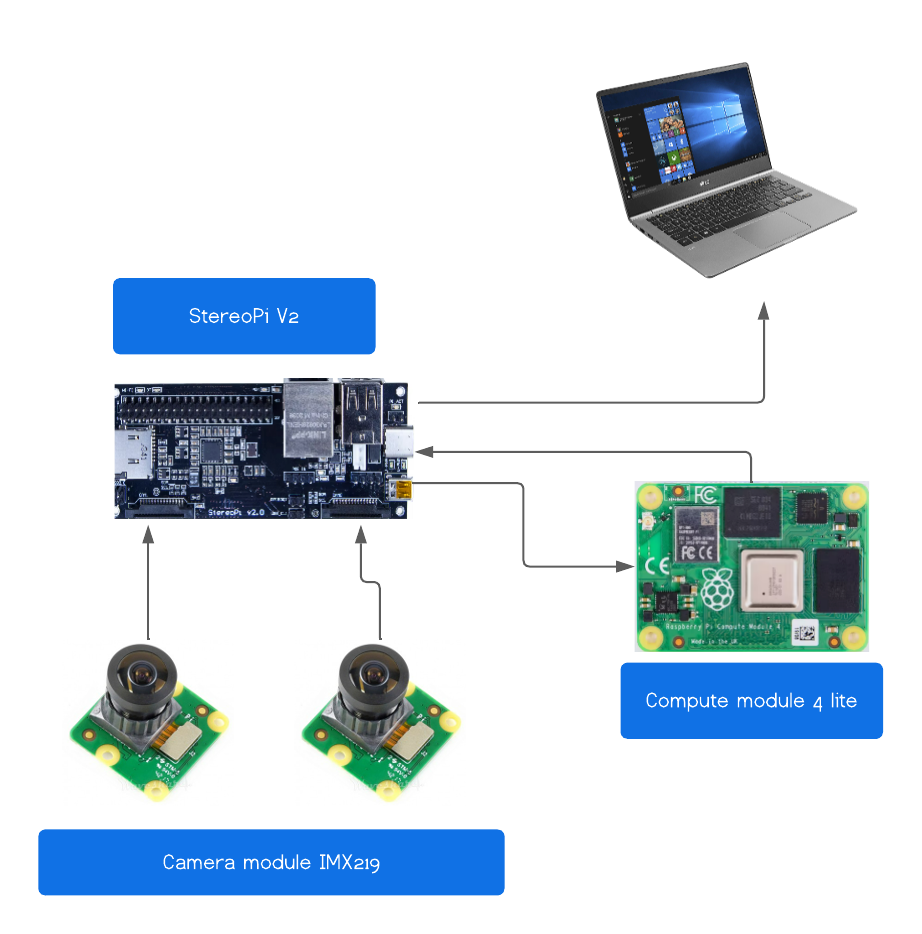
\includegraphics[scale=0.4]{Recursos/estrategia_stereopi_v2.png}
        \caption[Estrategia StereoPi V2.]{Estrategia StereoPi V2. {\footnotesize Fuente: El Autor}}
        \label{estrategia_v2}
     \end{subfigure}
     \hfill
\caption{Configuraciones basadas en módulo StereoPi}
\label{estrategias_stereopi}
\end{figure}
En la Tabla \ref{comparacion_stereopi} se presenta una comparación entre las características más importantes de las 3 estrategias.
\begin{table}[H]
\centering
\caption{Especificaciones de estrategias StereoPi}
\label{comparacion_stereopi}
\begin{tabular}{l|ccc|}
\cline{2-4}
 & \multicolumn{3}{c|}{Estrategias} \\ \hline
\multicolumn{1}{|l|}{Características} & \multicolumn{1}{c|}{StereoPi Slim} & \multicolumn{1}{c|}{StereoPi V1} & StereoPi V2 \\ \hline
\multicolumn{1}{|l|}{Wifi} & \multicolumn{1}{c|}{No} & \multicolumn{1}{c|}{No} & Si \\ \hline
\multicolumn{1}{|l|}{Bluetooth} & \multicolumn{1}{c|}{No} & \multicolumn{1}{c|}{No} & Si \\ \hline
\multicolumn{1}{|p{2.5cm}|}{CPU} & \multicolumn{1}{p{2.5cm}|}{ARM Cortex-A53 64-bit @ 1.2GHz} & \multicolumn{1}{p{2.5cm}|}{ARM Cortex-A53 64-bit @ 1.2GHz} &\multicolumn{1}{p{2.5cm}|}{ARM Cortex-A72 64-bit @ 1.5GHz} \\ \hline
\multicolumn{1}{|p{2.5cm}|}{RAM} & \multicolumn{1}{p{2.5cm}|}{1GB LPDDR2 SDRAM} & \multicolumn{1}{p{2.5cm}|}{1GB LPDDR2 SDRAM} & \multicolumn{1}{p{2.5cm}|}{2GB LPDDR4-3200 SDRAM} \\ \hline
\multicolumn{1}{|p{3cm}|}{Almacenamiento} & \multicolumn{1}{p{2.5cm}|}{micro SD} & \multicolumn{1}{p{2.5cm}|}{micro SD} & \multicolumn{1}{p{2.5cm}|}{micro SD } \\ \hline
\multicolumn{1}{|p{2.5cm}|}{Sistema operativo} & \multicolumn{1}{p{2.5cm}|}{Raspbian} & \multicolumn{1}{p{2.5cm}|}{Raspbian} & \multicolumn{1}{p{2.5cm}|}{Raspbian} \\ \hline
\multicolumn{1}{|p{2.5cm}|}{Ethernet} & \multicolumn{1}{c|}{No} & \multicolumn{1}{c|}{Si} & Si \\ \hline
\multicolumn{1}{|p{2.5cm}|}{HDMI} & \multicolumn{1}{c|}{Si} & \multicolumn{1}{c|}{Si} & Si \\ \hline
\multicolumn{1}{|p{2.5cm}|}{USB} & \multicolumn{1}{c|}{1 x micro} & \multicolumn{1}{c|}{2 x Tipo A, 1 x micro} & 2 x Tipo A, 1 x Tipo C \\ \hline
\multicolumn{1}{|p{2.5cm}|}{Video} & \multicolumn{1}{p{2.5cm}|}{1080p30, 720p60 y 640x480p90} & \multicolumn{1}{p{2.5cm}|}{1080p30, 720p60 y 640x480p90} & \multicolumn{1}{p{2.5cm}|}{1080p30, 720p60 y 640x480p90} \\ \hline
\multicolumn{1}{|p{2.5cm}|}{Resolución de cámara} & \multicolumn{1}{c|}{5 MP} & \multicolumn{1}{p{2.5cm}|}{5 MP} & 8 MP \\ \hline
\end{tabular}
\end{table}
\subsection{Estrategia con Jetson Nano B01 y módulo IMX219-83}
Como su nombre lo indica esta emplea un módulo Jetson Nano B01 cuyas cualidades relevantes son:
\begin{itemize}
    \item \textbf{GPU:} 128 núcleos con la arquitectura Maxwell de NVIDIA.
    \item \textbf{CPU:} ARM 57 Quad-core.
    \item \textbf{Memoria RAM:} 4 GB LPDDR4.
    \item \textbf{Entradas/salidas:} Ethernet, 4 USB 3.0, micro USB, HDMI, UART, I2C, SPI, 2 puertos MIPI-CSI (conectores de cámaras).
\end{itemize}
El módulo IMX219-83 es un integrado que contiene dos cámaras, acompañadas del chip ICM20948, sin embargo a continuación se listarán las características únicamente del elemento estéreo:
\begin{itemize}
    \item \textbf{Megapíxeles:} 8 MP.
    \item \textbf{Resolución:} 3280 × 2464 px (por cámara).
    \item \textbf{FOV:} 83/73/50 grados (diagonal/horizontal/vertical).
    \item \textbf{Distancia focal:} 2.6 mm
    \item \textbf{Línea base:} 60 mm.
\end{itemize}
En la Figura \ref{estrategia_jetson} se puede observar un diagrama que representa como se aplicaría esta estrategia.
\begin{figure}[H]
    \centering
    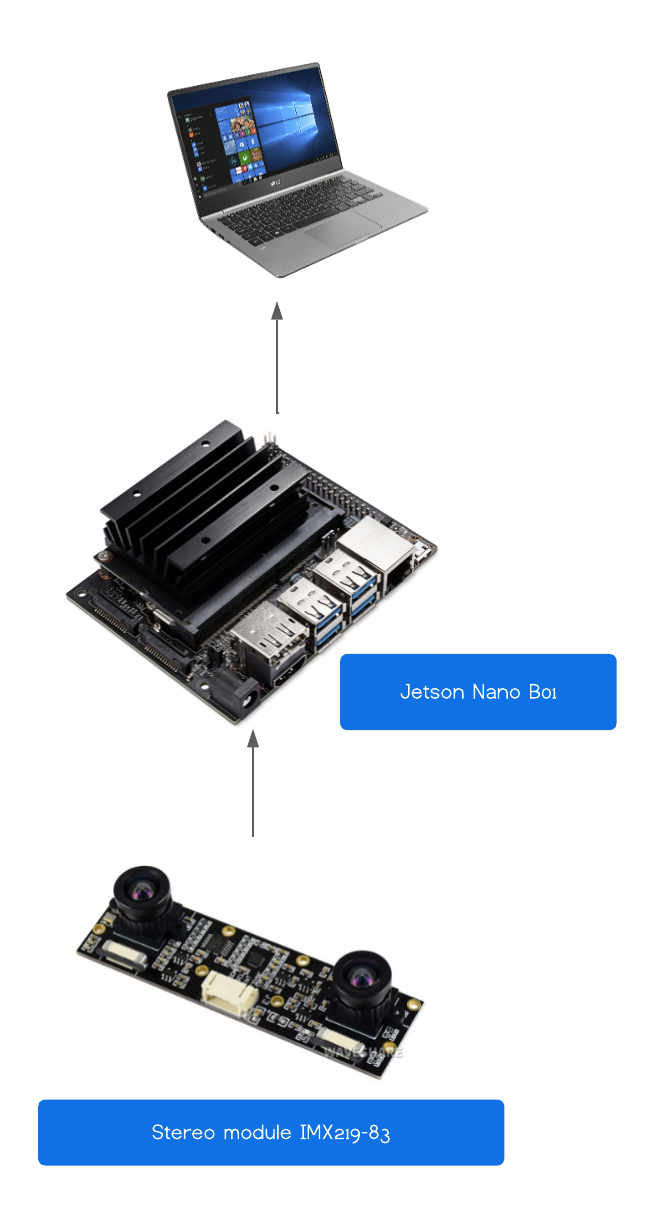
\includegraphics[scale=0.5]{Recursos/estrategia_jestson_nano.png}
    \caption[Estrategia con Jetson Nano B01.]{Estrategia con Jetson Nano B01. {\footnotesize Fuente: El Autor}}
    \label{estrategia_jetson}
\end{figure}
\subsection{Estrategia con dos teléfonos}
Usando las cámaras de dos teléfonos a los cuales el autor tiene acceso y transmitiendo lo que observa cada cámara a un servidor local para captar ambas imágenes mediante el computador el cual realizara todo el procesamiento, es posible crear un sistema estéreo como el de la Figura \ref{estrategia_phone}.
\begin{figure}[H]
    \centering
    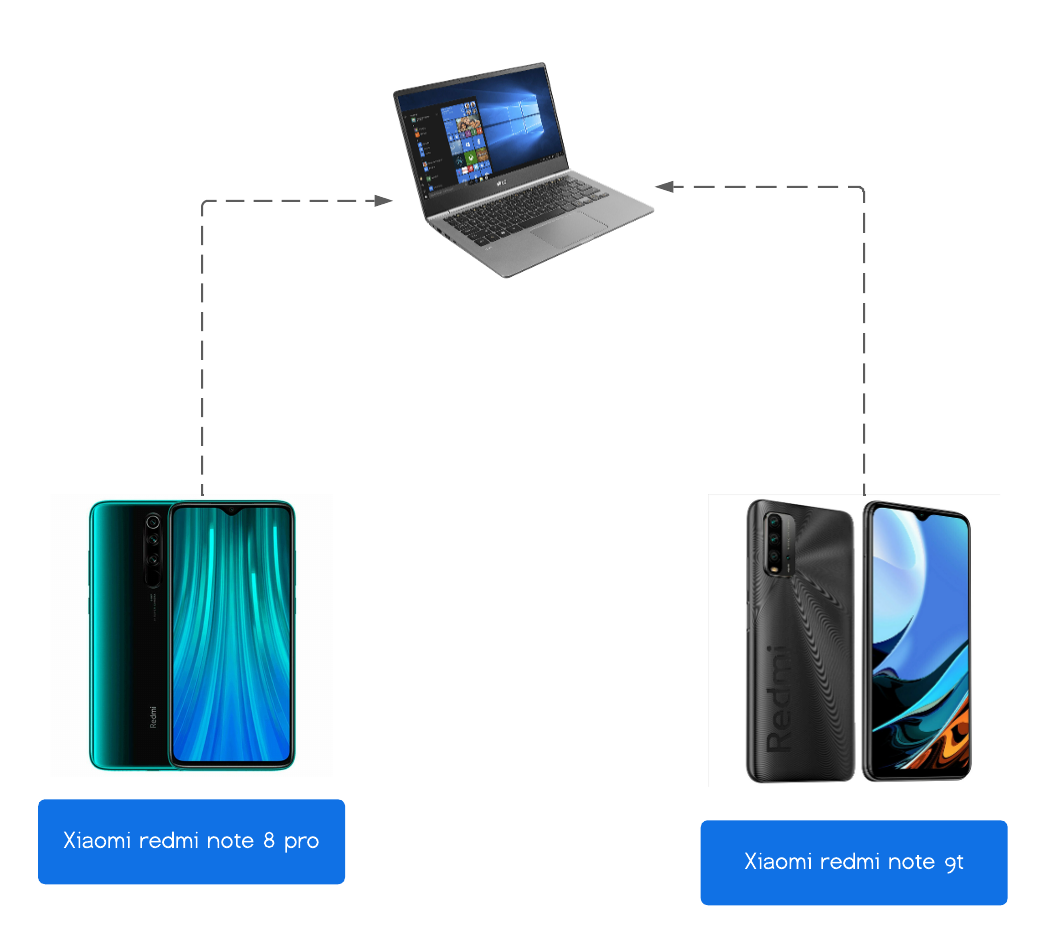
\includegraphics[scale=0.5]{Recursos/estrategia_telefonos.png}
    \caption[Estrategia con teléfonos.]{Estrategia con teléfonos. {\footnotesize Fuente: El Autor}}
    \label{estrategia_phone}
\end{figure}
Los teléfonos presentes en la Figura \ref{estrategia_phone} poseen las siguientes características:
\begin{itemize}
    \item Xiaomi redmi note 8 pro: sus dimensiones son 161.3 x 76.4 x 8.8 mm, posee 5 cámaras, con una resolución máxima de 64 MP.
    \item Xiaomi redmi 9T: sus dimensiones son 162.3 x 77.3 x 9.6 mm, posee 5 cámaras, con una resolución máxima de 48 MP.
\end{itemize}
\subsection{Elección de estrategia}
\begin{figure}[H]
    \centering
    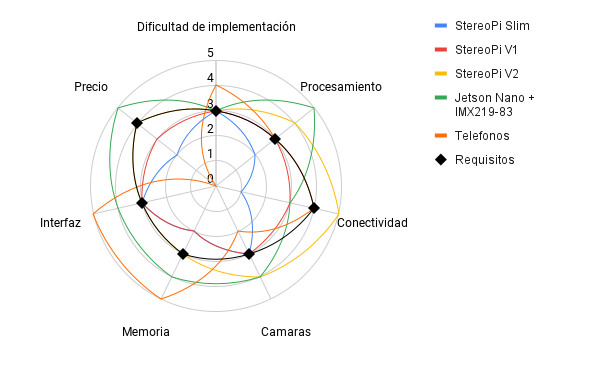
\includegraphics[scale=0.5]{Recursos/spyder_chart.png}
    \caption[Comparación de estrategias.]{Comparación de estrategias. {\footnotesize Fuente: El Autor}}
    \label{spyder_chart}
\end{figure}
En la Figura \ref{spyder_chart} se observan 7 parámetros que sintetizan las características requeridas expuestas anteriormente, por lo que a continuación se explicaran las razones de las puntuaciones obtenidas.
\begin{itemize}
    \item \textbf{Dificultad de implementación:} este parámetro permite medir que tan sencillo seria integrar todos los elementos de la estrategia, con el objetivo de poner en funcionamiento el sistema y probar las herramientas del paquete, en este caso es conveniente que sea sencillo, para así poder concentrar el trabajo en el paquete y no en la implementación física, como se puede observar en la Figura \ref{spyder_chart} el más complicado de implementar es el que emplea teléfonos, puesto que requiere diseñar y construir una estructura que pueda soportar ambos teléfonos y que a su vez ubique perfectamente los centros ópticos en una disposición paralela.
    \item \textbf{Procesamiento:} relacionado con la capacidad del CPU y la GPU en el caso de la Jetson Nano, ya que esta permite ejecutar modelos de aprendizaje automático de forma más eficiente. Como se puede observar en la Figura \ref{spyder_chart} al menos 4 de 5 son capaces de cumplir con este parámetro.
    \item \textbf{Conectividad:} este se relaciona con las formas de poder conectarse con el computador donde se esta desarrollando el paquete y dado que el StereoPi V2 posee conexión mediante wifi es posible probar como funciona el paquete cuando las imágenes son enviadas de forma remota al igual que con dos dispositivos móviles.
    \item \textbf{Cámaras:} esto va ligado tanto a la calidad de la imagen y el vídeo, como al hecho de que ambas cámaras tengan características similares, razón por la cual la opción de los teléfonos se ve fuertemente penalizada, porque si bien es cierto que es posible realizar estéreo con cámaras distintas y sin conocer los parámetros, también es correcto decir que calibrar los parámetros intrínsecos e extrínsecos de teléfonos distintos puede llevar a un mayor error al momento de hallar el mapa de disparidad.
    \item \textbf{Memoria:} el método elegido debe ser capaz de poder almacenar las librerías que se utilizan en el paquete.
    \item \textbf{Interfaz:} a mayor puntación será más sencillo implementar el paquete, razón del porqué la opción de los teléfonos tiene el valor máximo, ya que; de emplearla el procesamiento es realizado mediante el computador, por lo que no sería necesario diseñar una app móvil, ya que existen aplicaciones como IP webcam que permiten crear un servidor local y transmitir vídeo a este.
    \item \textbf{Precio:} un factor tan relevante como los anteriores al momento de dimensionar cualquier sistema.
\end{itemize}
Como se puede observar en la Figura \ref{spyder_chart} el método con teléfonos tiene un precio de 0, debido a que ya se poseen ambos dispositivos e incluso el resto de sus puntuaciones son bastante buenas a excepción del esfuerzo que implica construir la estructura de soporte; sin embargo, dicha opción tiene un problema que impediría el correcto funcionamiento del sistema y esa es su puntuación en las cámaras, por otro lado si bien el módulo de desarrollo de NVIDIA cumple excepcionalmente en casi todo, su costo es muy elevado y no posee comunicación inalámbrica por lo que para poder comprobar el funcionamiento de todo el paquete sería necesario agregar un módulo de wifi aparte, lo que elevaría aún más el costo final. En el caso del StereoPi V1 posee el mismo problema de conectividad y puede que su memoria sea insuficiente e incluso la capacidad de procesamiento queda ajustada. Por estos motivos se seleccionó la estrategia StereoPi V2.  
\subsection{Implementación del sistema de adquisición de datos}
Para poder armar la estrategia seleccionada no solo fueron necesarios los elementos ya mencionados, debido a que el soporte físico sobre el que se sustentaría el StereoPi y el Compute Module 4 lite era un componente de vital importancia para poder mantener el conjunto de cámaras en una posición fija, a tal efecto se empleó una montura como el que utilizan las cámaras GoPro, (Ver Figura \ref{gopro_support}) la cual está compuesta de 3 partes una arandela, 1 tornillo para ajustar y un trípode.
\begin{figure}[H]
    \centering
    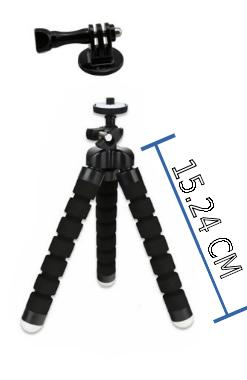
\includegraphics[scale=0.5]{Recursos/go_pro_support.jpg}
    \caption[Montura del sistema tipo GoPro.]{Montura del sistema tipo GoPro. {\footnotesize Fuente: El Autor}}
    \label{gopro_support}
\end{figure}
\subsubsection{Ensamblado}
Se siguieron los siguientes pasos para armar el sistema:
\begin{enumerate}
    \item Se posicionaron el módulo StereoPi V2 y el CM4 lite como en la Figura \ref{connect_cm4} y posteriormente se conectaron.
    \begin{figure}[H]
        \centering
        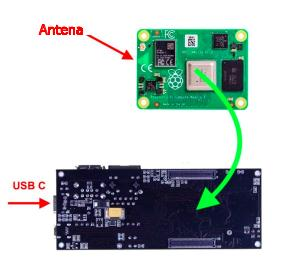
\includegraphics{Recursos/cm4_connect.jpg}
        \caption[Conexión entre CM4 lite y StereoPi V2.]{Conexión entre CM4 lite y StereoPi V2. {\footnotesize Fuente: \textit{StereoPi v2 Quick Start Guide} \cite{realizator_2021}}}
        \label{connect_cm4}
    \end{figure}
    \item Se insertó una tarjeta SD de 32 GB en el StereoPi V2, aunque para permitir el acceso a dicha memoria con el fin de programar, se le colocaron 3 jumpers al StereoPi V2 que cortocircuitan los pines RPIBOOT, USB \textit{slave} y \textit{power switch}, los cuales se localizan como en la Figura \ref{stereoPi_IO}
    \begin{figure}[H]
        \centering
        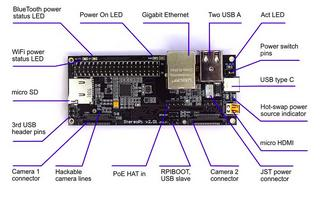
\includegraphics{Recursos/stereoPi_IO.jpg}
        \caption[Entradas y salidas del StereoPi V2.]{Entradas y salidas del StereoPi V2. {\footnotesize Fuente: \textit{StereoPi v2 Quick Start Guide} \cite{realizator_2021}}}
        \label{stereoPi_IO}
    \end{figure}
    \item Con uno de los moldes impresos en acrílico, 4 tuercas y 4 espaciadores de 10 mm se armó la base de las cámaras como en la Figura \ref{camera_base}.
    \begin{figure}[H]
        \centering
        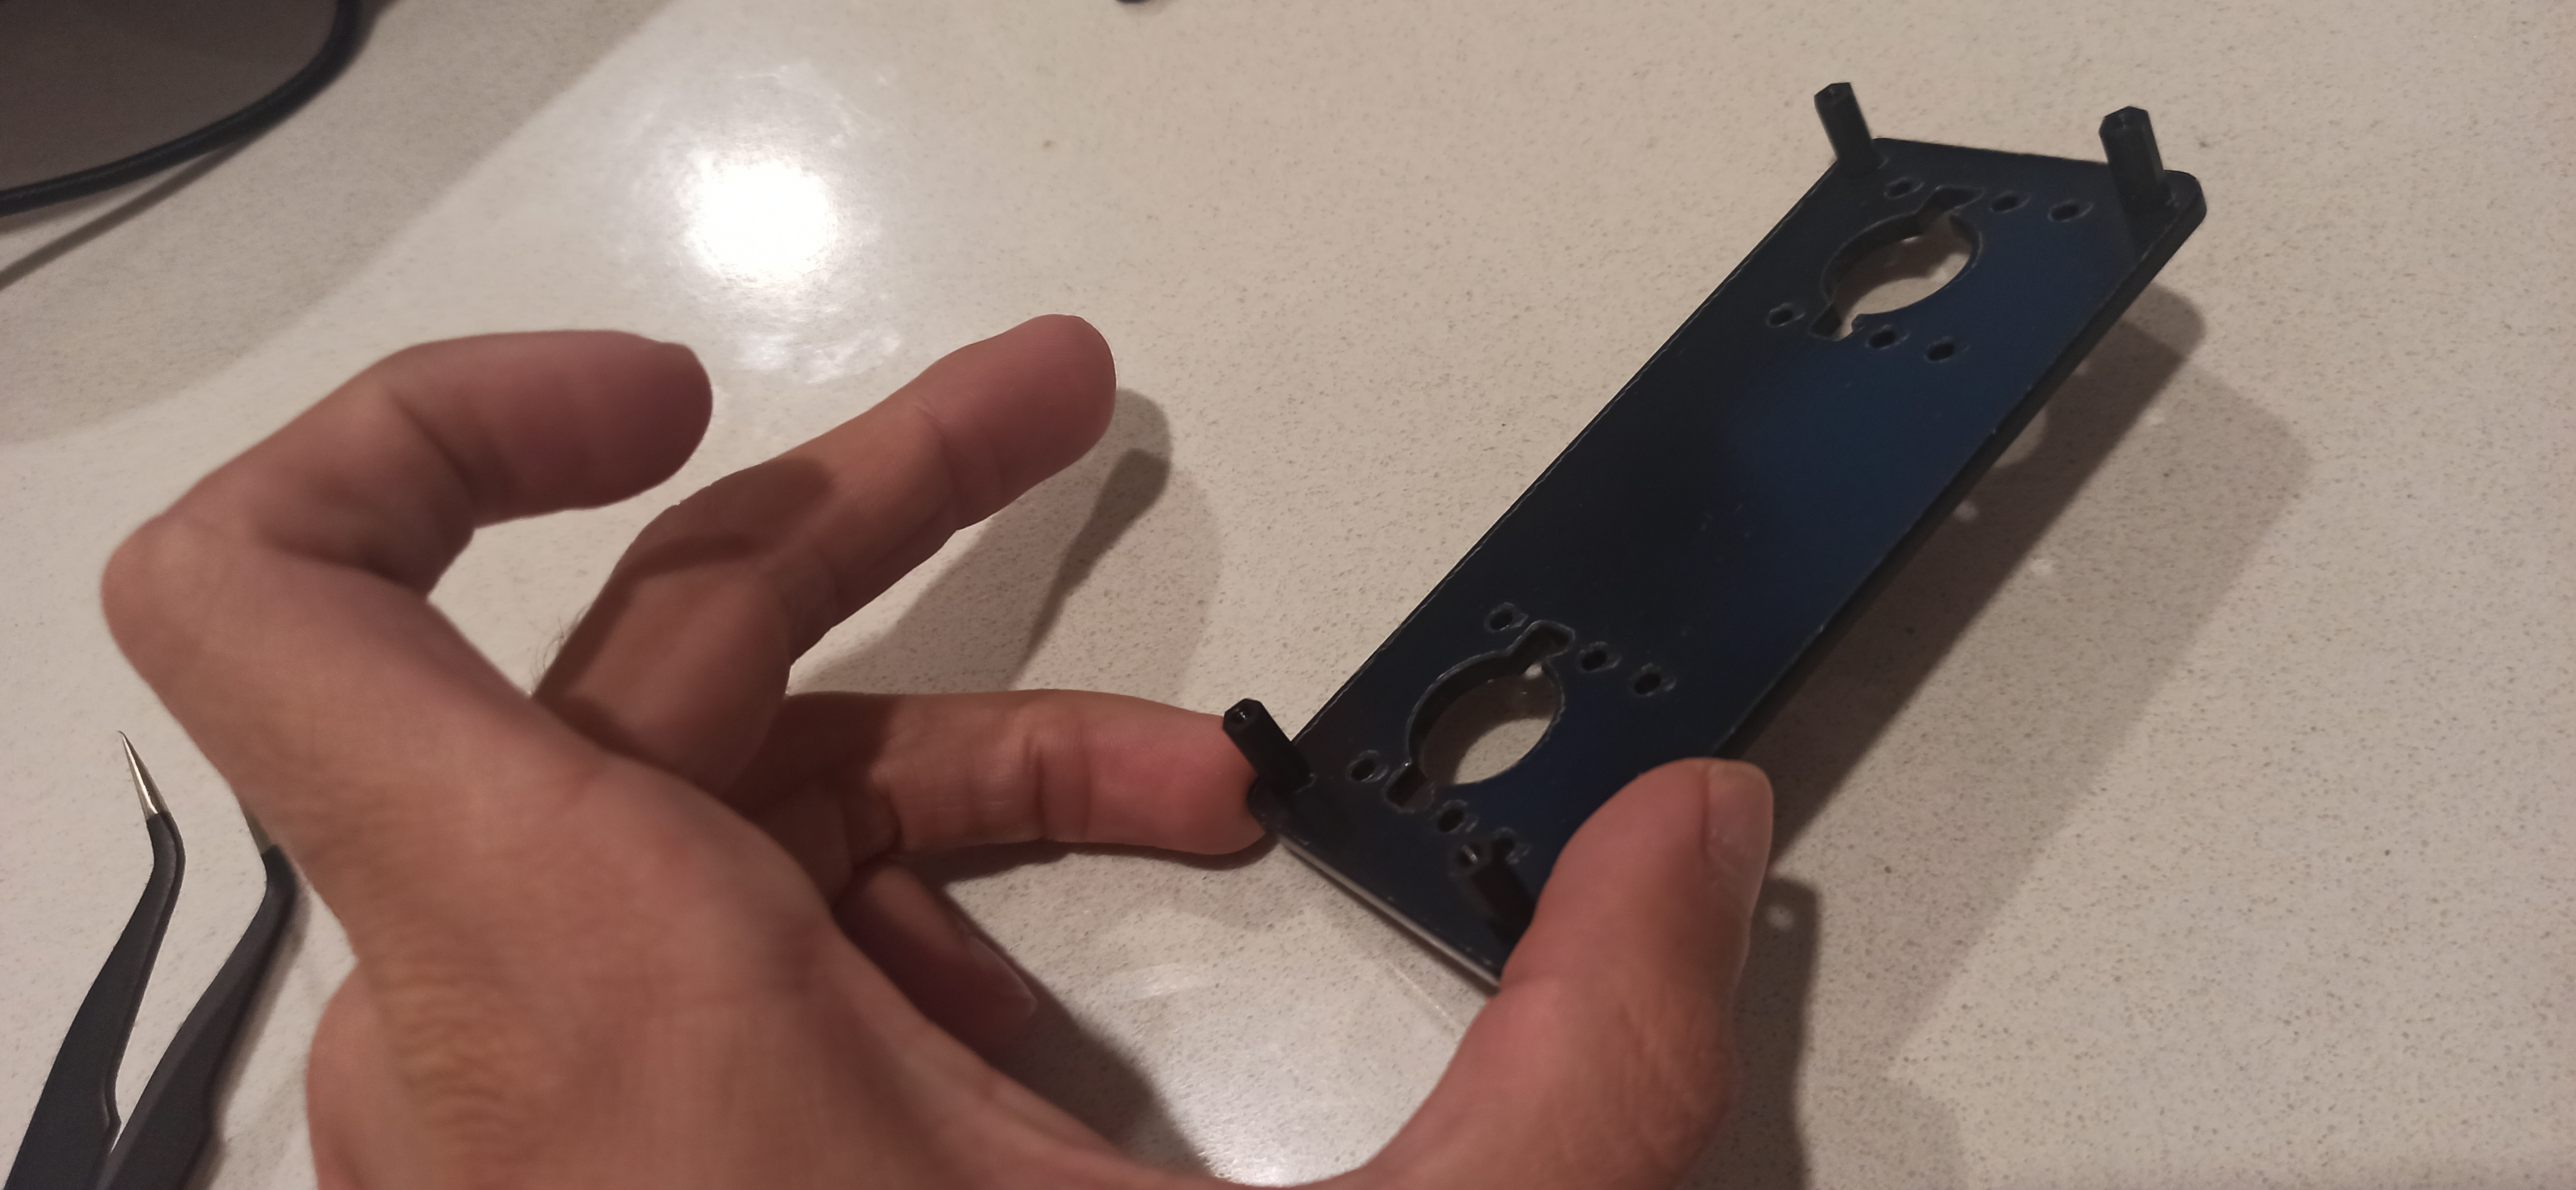
\includegraphics[scale=0.05]{Recursos/camera_base.jpg}
        \caption[Base de las cámaras IMX219 instalada.]{Base de las cámaras IMX219 instalada. {\footnotesize Fuente: El Autor}}
        \label{camera_base}
    \end{figure}
    \item A la base armada en el paso previo se le acoplaron 2 cámaras IMX219 con 8 tornillos y 8 tuercas (ver Figura \ref{cameras_installed}). Las cámaras cuentan con una resolución de 8 MP, pueden captar imágenes de hasta 3280 x 2464 píxeles, transmitir vídeo con una resolución y cuadros por segundo de 1080p30, 720p60 y 640x480p90, son compatibles con interfaces CSI (Camera Serial Interface), poseen un \textit{Field of view} (FOV) de 160$^0$, cuentan con un lente con una apertura de 2.35 y una distancia focal de 3.15 mm.
    \begin{figure}[H]
        \centering
        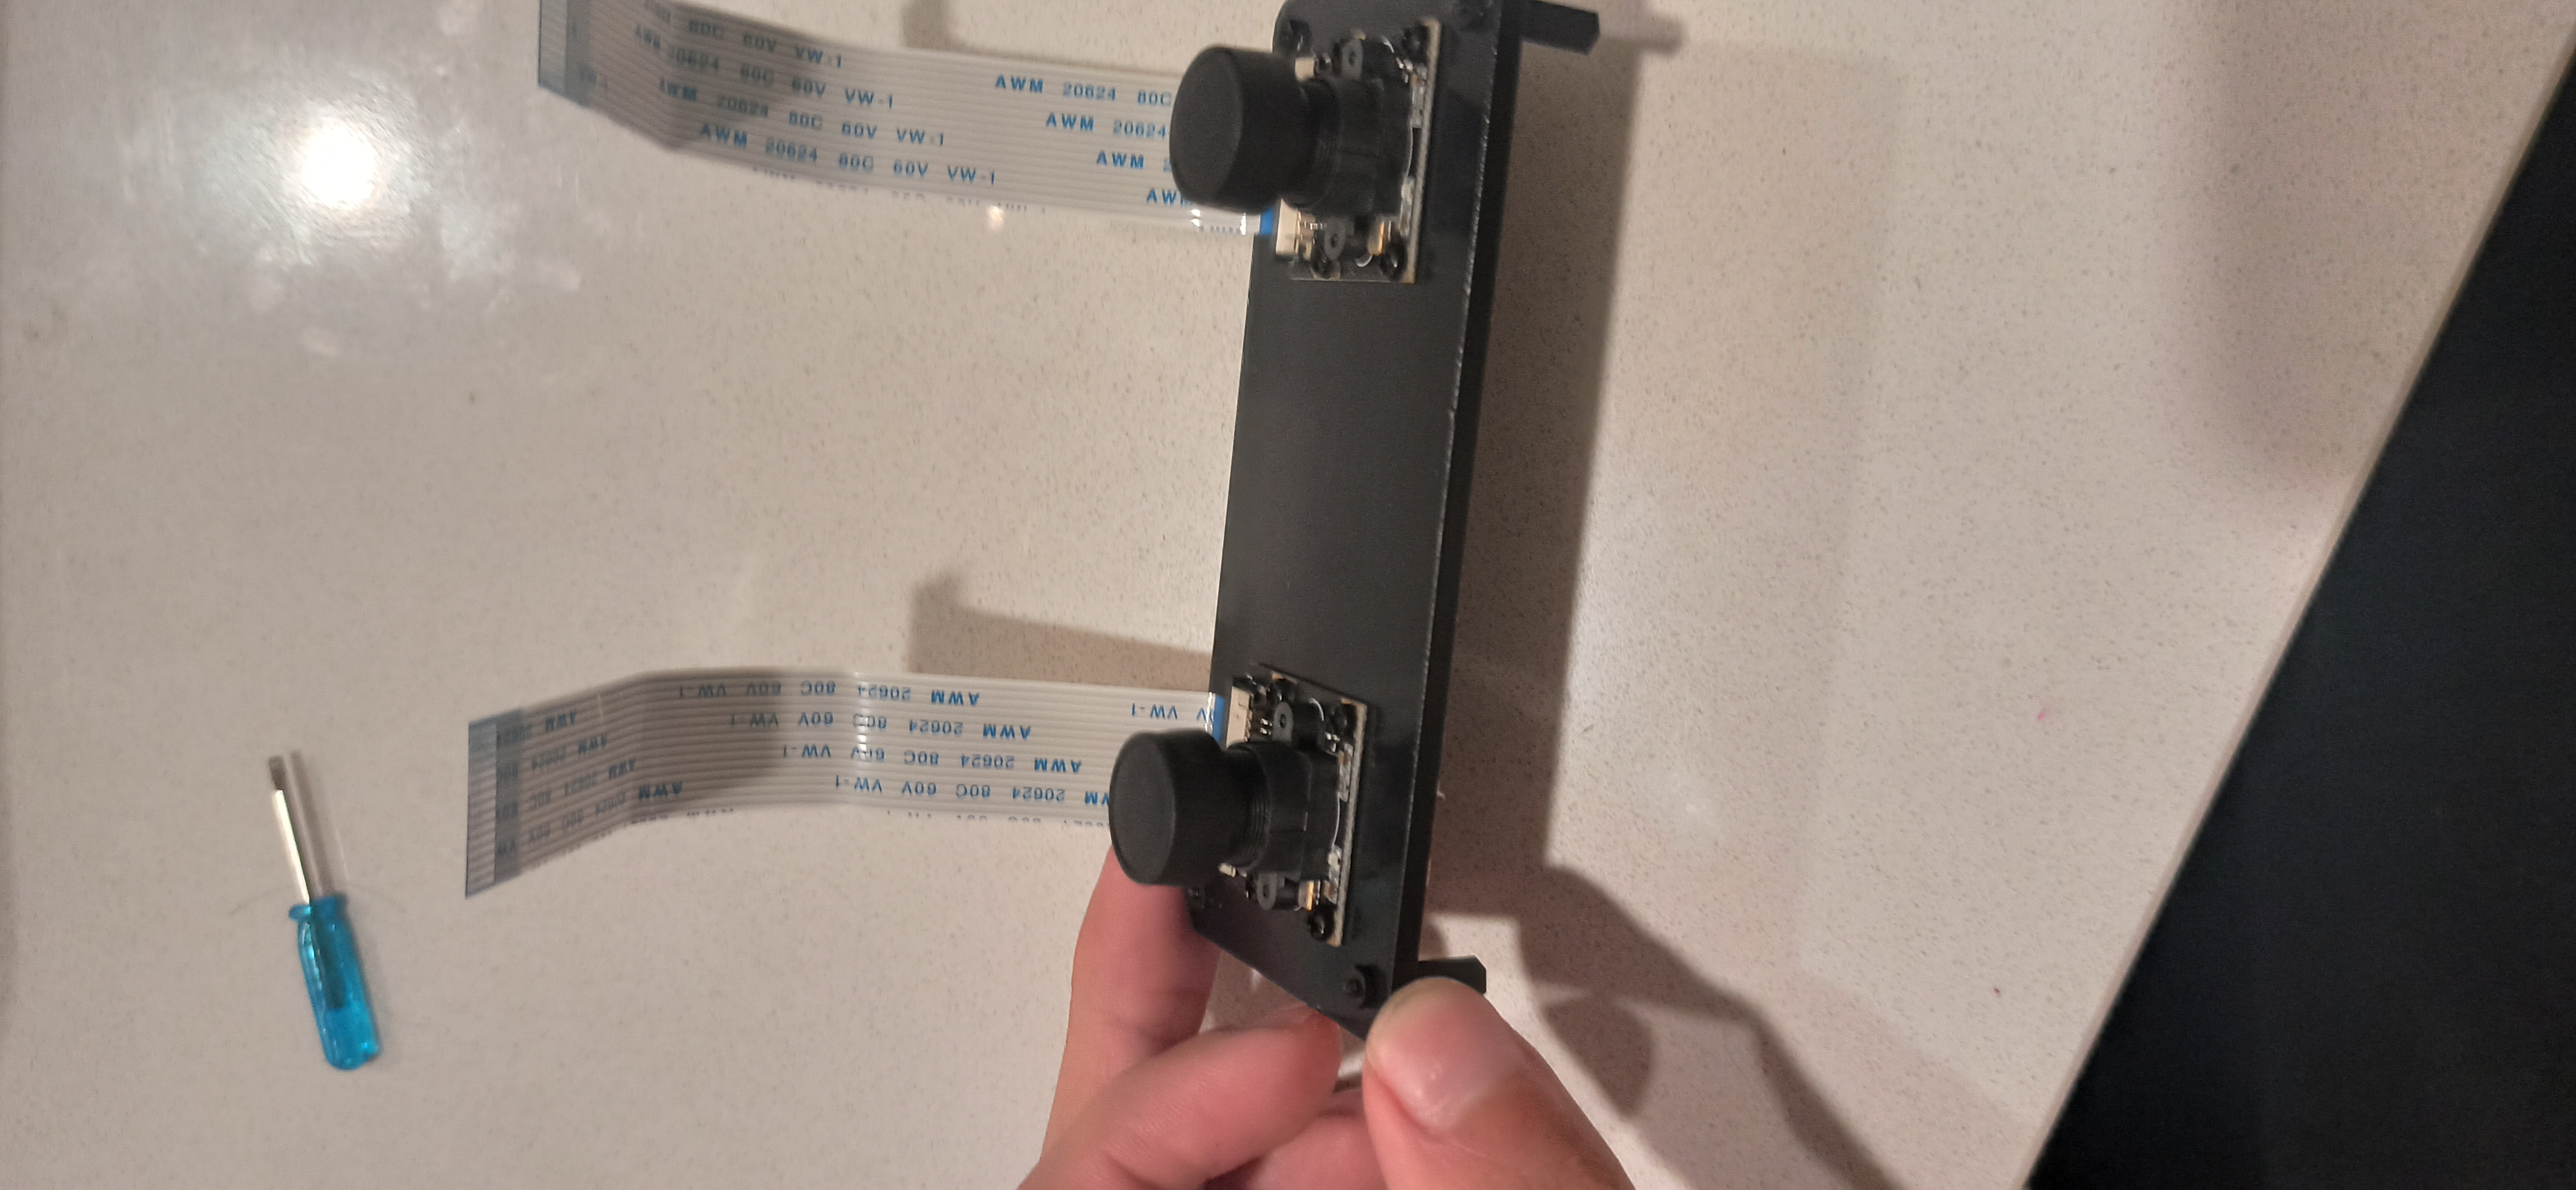
\includegraphics[scale=0.05]{Recursos/camera_installed.jpg}
        \caption[Módulos IMX219 instalados.]{Módulos IMX219 instalados. {\footnotesize Fuente: El Autor}}
        \label{cameras_installed}
    \end{figure}
    \item Se conectaron las cámaras al módulo estéreo y se ensambló el último a la base de las cámaras con 4 espaciadores de 20 mm como en la Figura \ref{module_installed}.
    \begin{figure}[H]
        \centering
        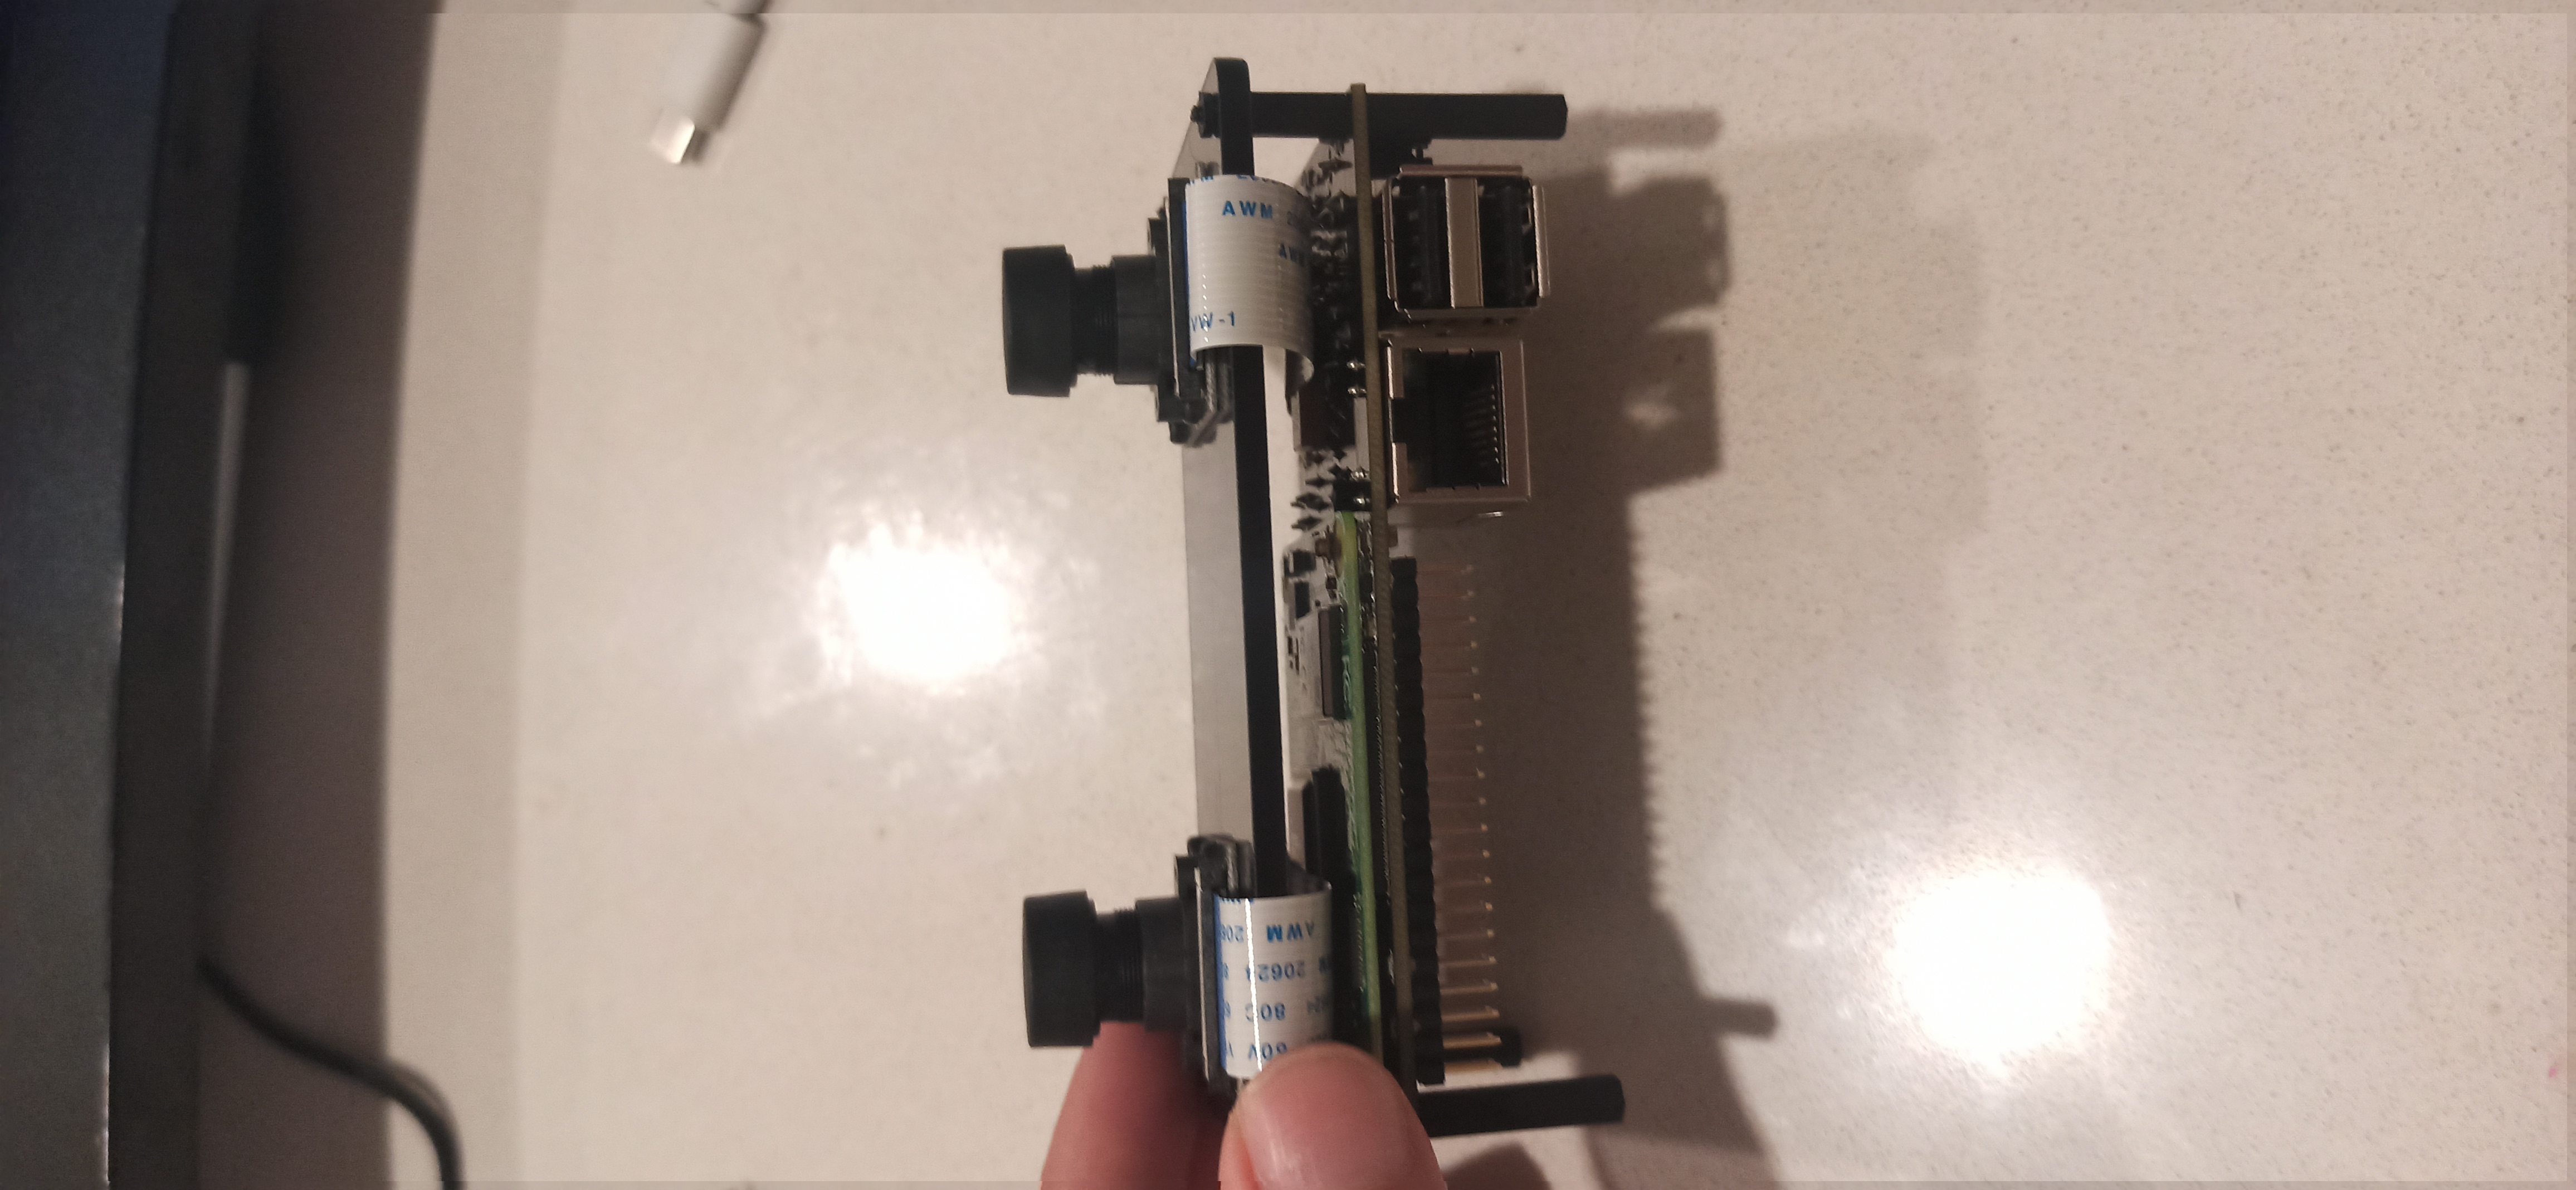
\includegraphics[scale=0.05]{Recursos/module_installed.jpg}
        \caption[IMX219 acoplados al StereoPi V2 y compute module 4 lite.]{IMX219 acoplados al StereoPi V2 y compute module 4 lite. {\footnotesize Fuente: El Autor}}
        \label{module_installed}
    \end{figure}
    \item Para fijar todas las piezas y poder conectar la estructura con la montura de la GoPro se conectó la otra pieza de acrílico con 4 tornillos al igual que en la Figura \ref{two_acrilics}.
    \begin{figure}[H]
        \centering
        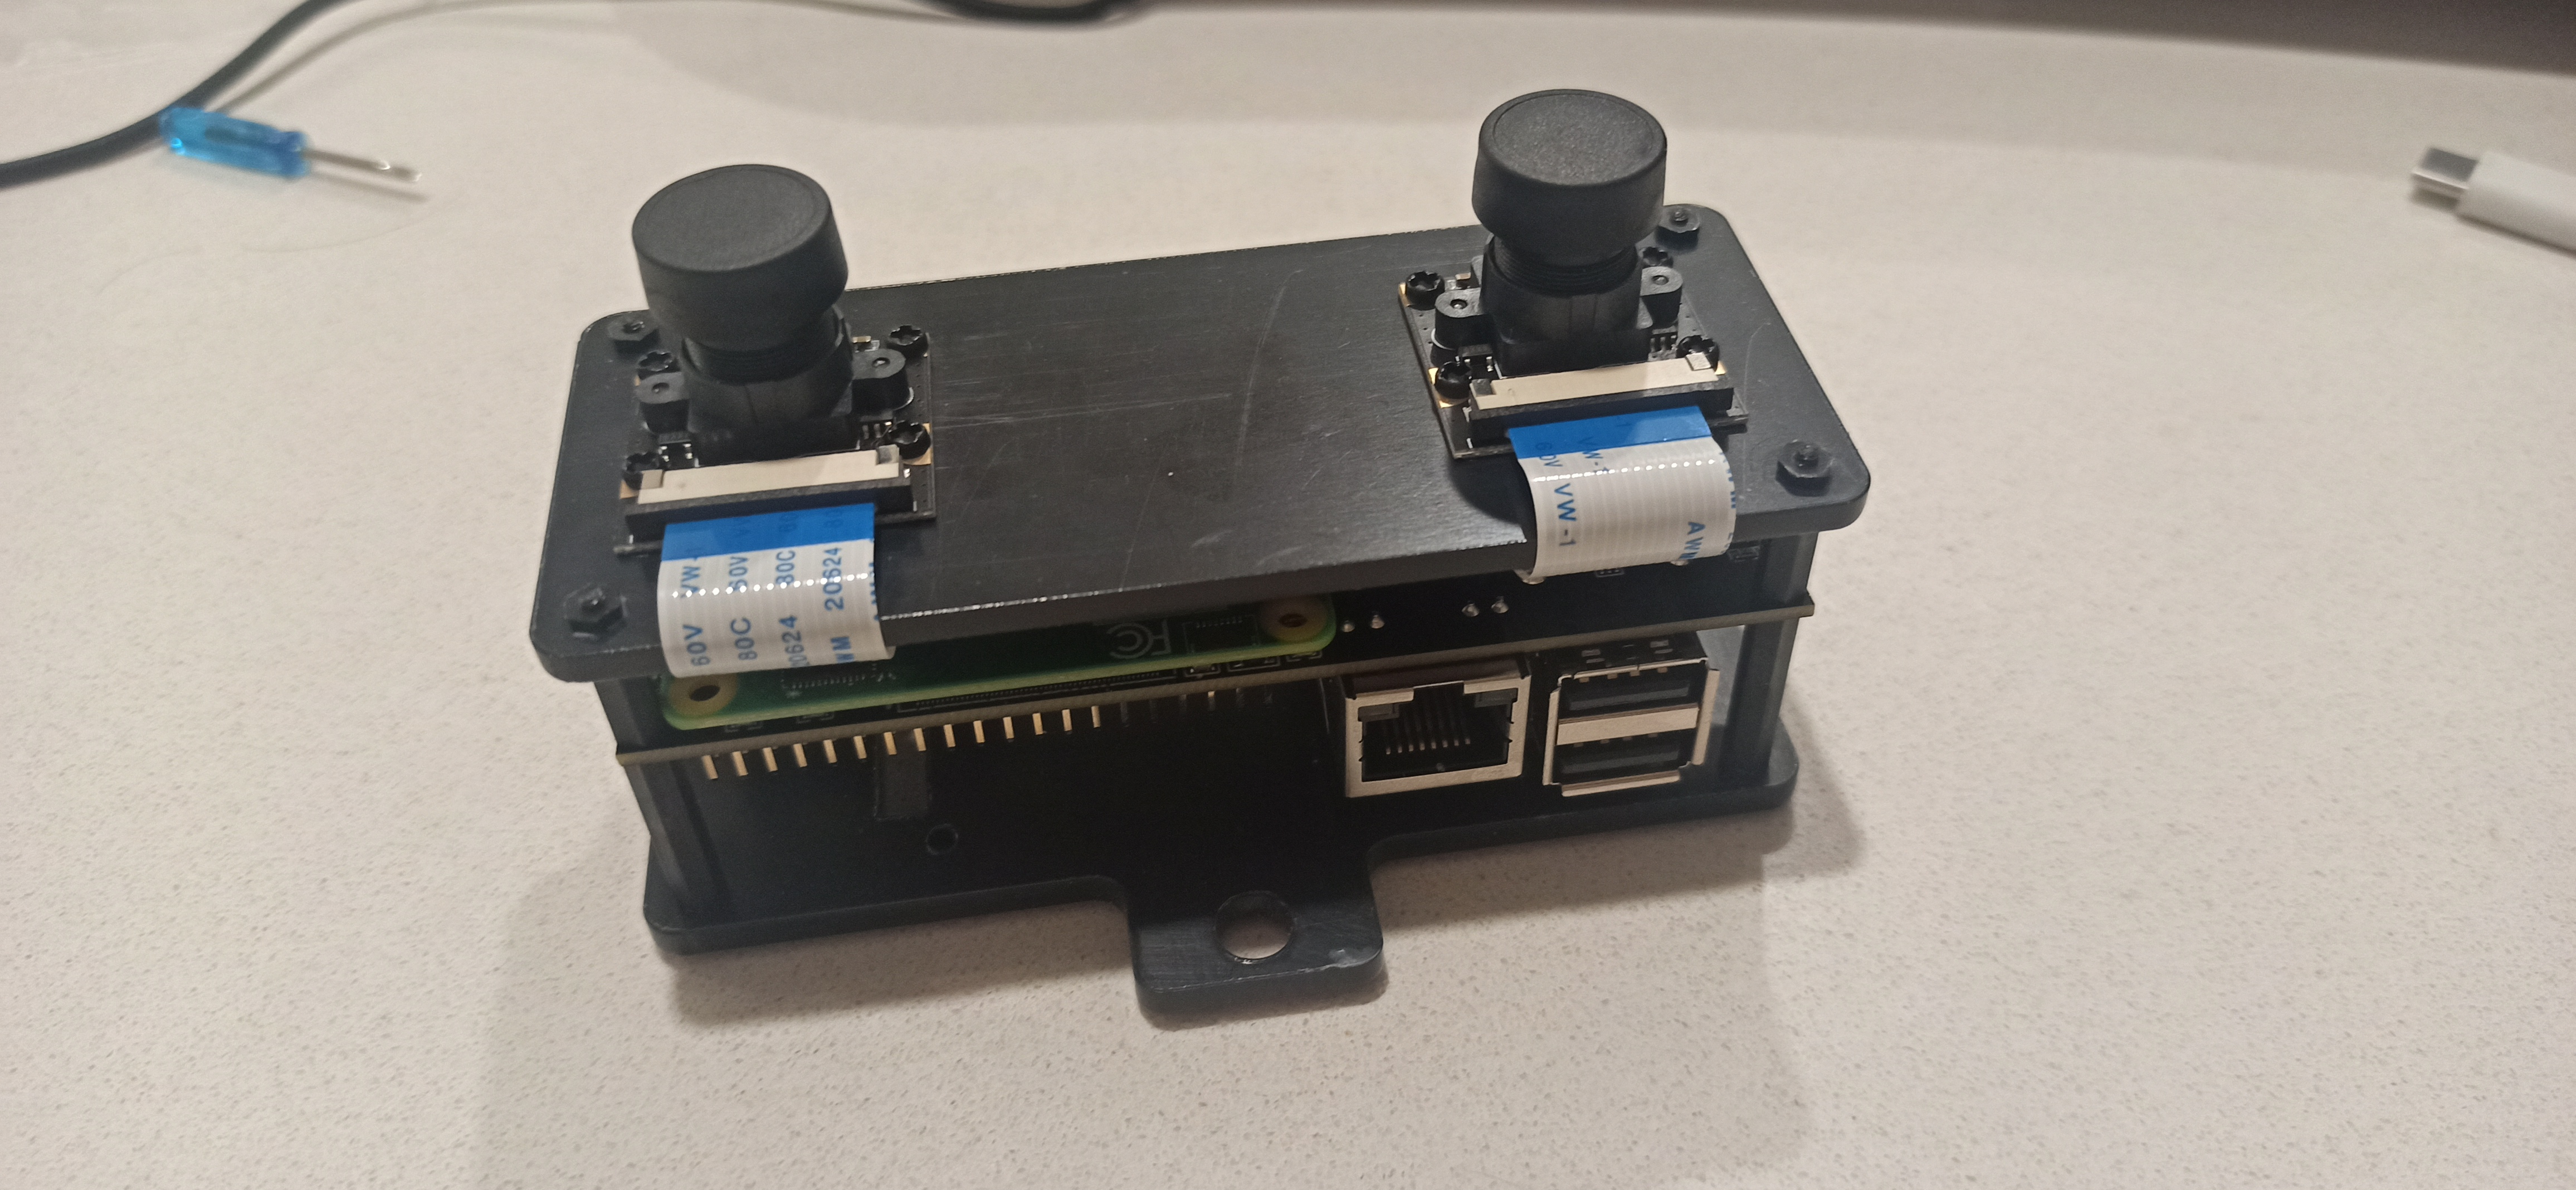
\includegraphics[scale=0.05]{Recursos/two_pastic_installed.jpg}
        \caption[Estructura de adquisición de datos sin montura.]{Estructura de adquisición de datos sin montura. {\footnotesize Fuente: El Autor}}
        \label{two_acrilics}
    \end{figure}
    \item Se conectó la estructura con la montura de la GoPro (ver Figura \ref{implemented_stereo_pi}).
    \begin{figure}[H]
        \centering
        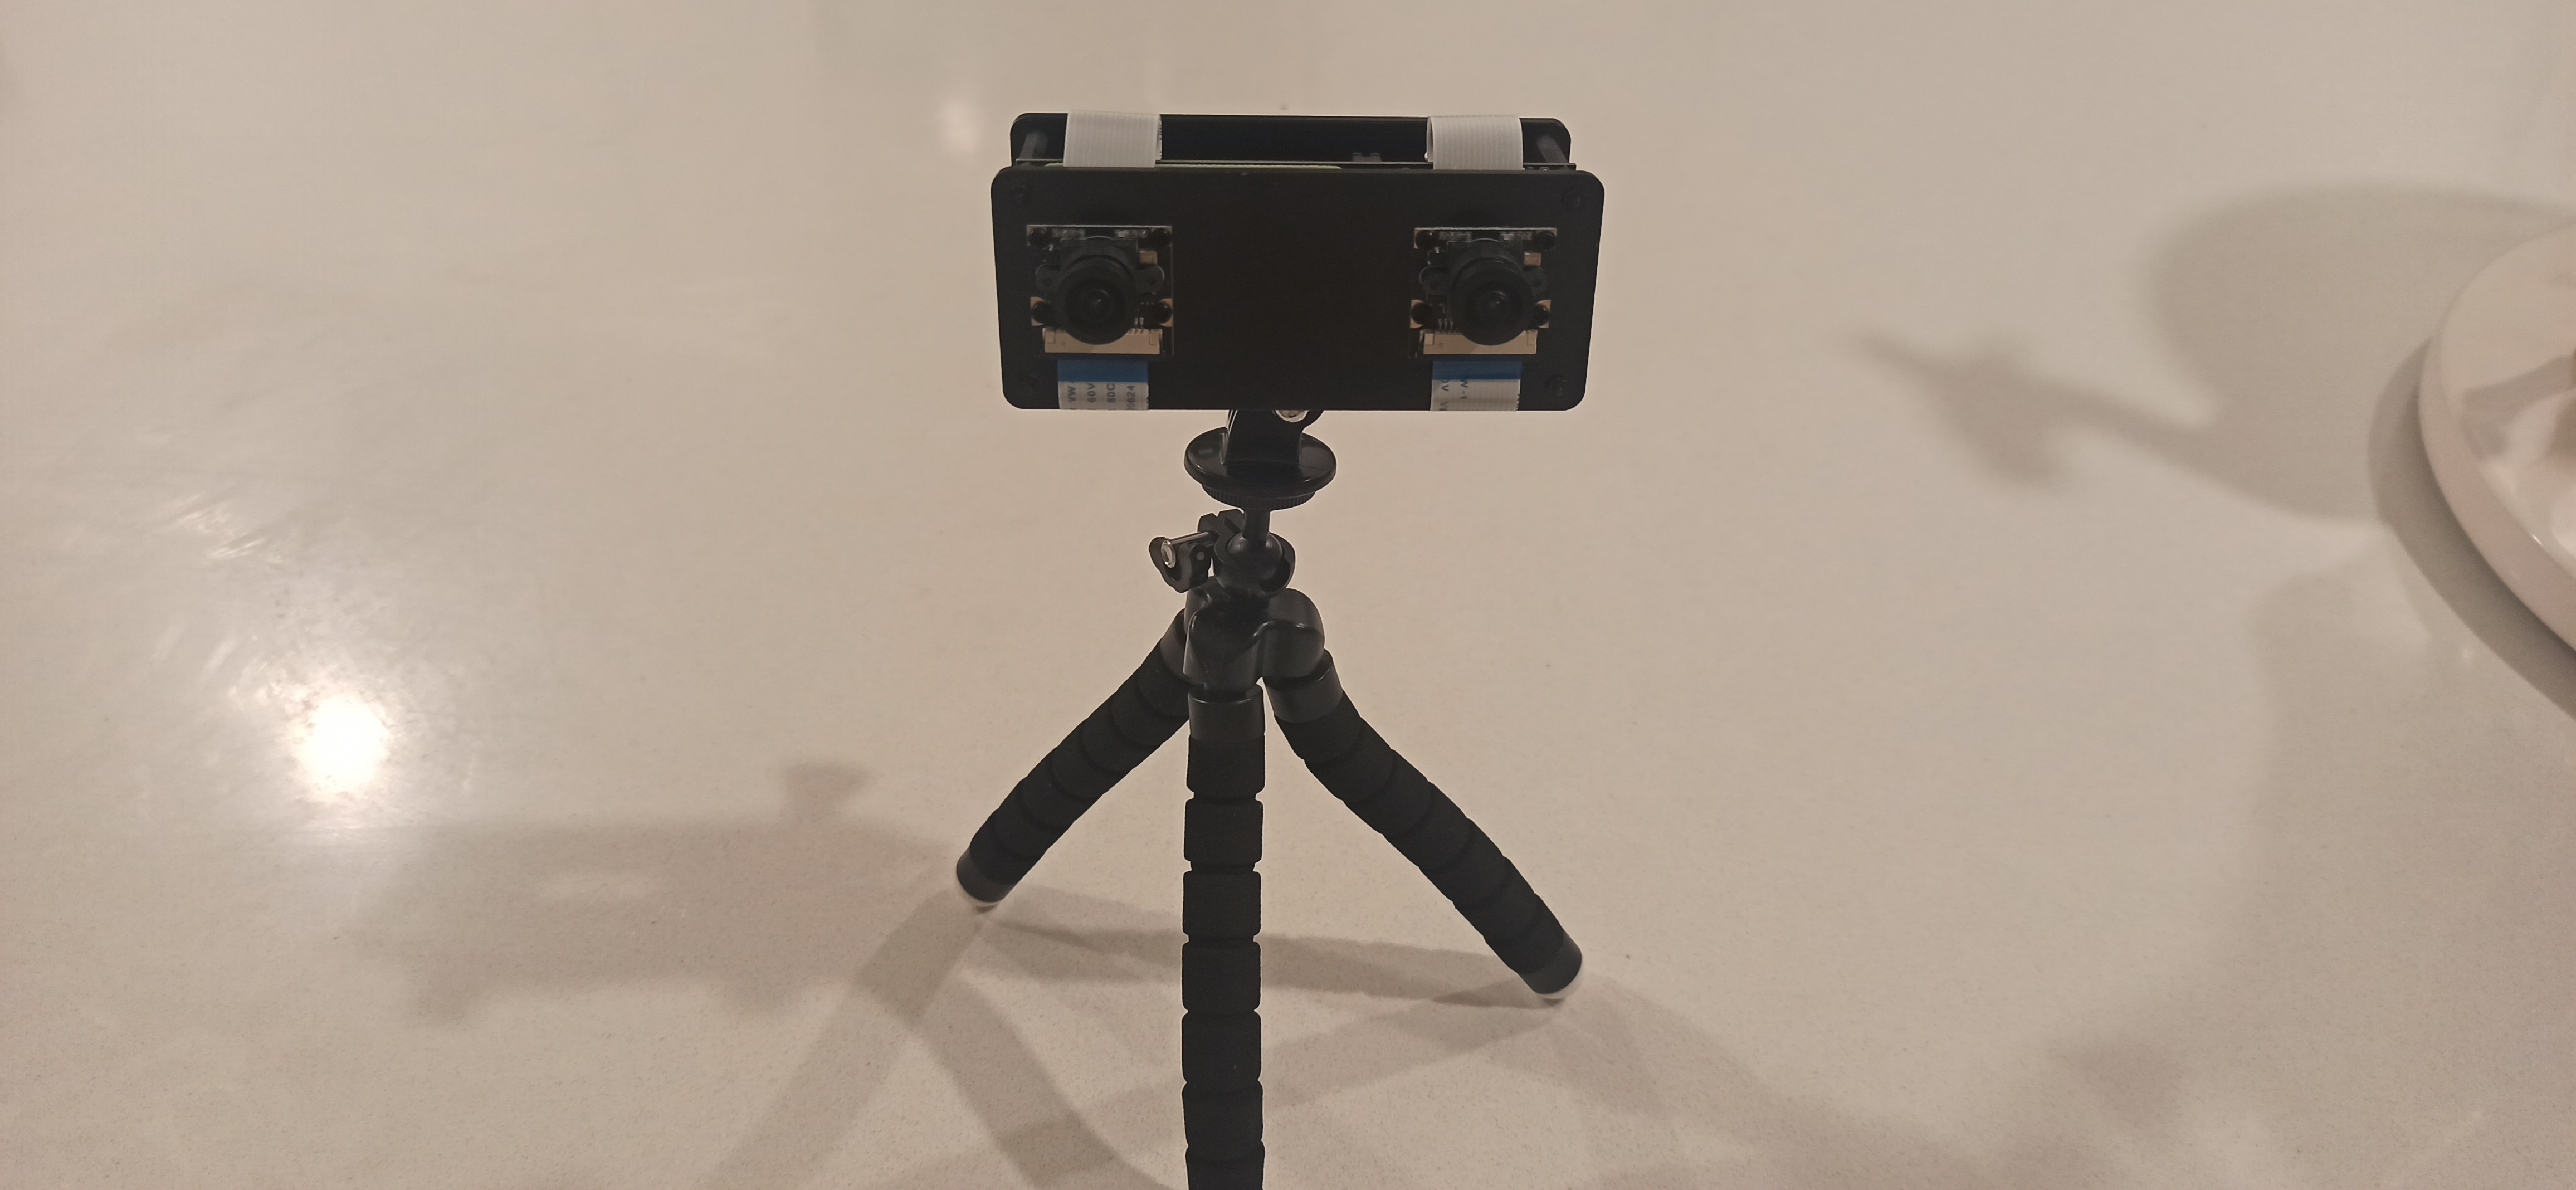
\includegraphics[scale=0.05]{Recursos/implemented_stereopiv2.jpg}
        \caption[Implementación del sistema.]{Implementación del sistema. {\footnotesize Fuente: El Autor}}
        \label{implemented_stereo_pi}
    \end{figure}
    \item Adicionalmente se le anexó una antena al CM4 lite para comprobar las funciones inalámbricas del paquete.
\end{enumerate}
En la tabla \ref{BOM} se listan los materiales empleados para la implementación del sistema.
\begin{table}[H]
\centering
\caption{Lista de materiales}
\label{BOM}
\begin{tabular}{|c|c|c|}
\hline
Cantidad & Ítem                           & Características             \\ \hline
1        & Módulo StereoPi                & Versión 2.02                \\ \hline
1        & Memoria SD                     & 32 GB                       \\ \hline
1        & Raspberry Pi Compute Module 4  & Versión lite                \\ \hline
2        & Cámara IMX-219                 & FOV 160$^0$                \\ \hline
2        & Pieza de acrílico              & -                           \\ \hline
3        & Jumper para cortocircuitar PCB & -                           \\ \hline
1        & Montura de GoPro               & 15.24 cm                    \\ \hline
4        & Espaciador                     & 20 mm                       \\ \hline
4        & Espaciador                     & 10 mm                       \\ \hline
12       & Tuercas                        & plástico                    \\ \hline
12       & Tornillos                      & Tipo cruz                   \\ \hline
1        & Antena                         & -                           \\ \hline
1        & USB                            & Tipo C                      \\ \hline
\end{tabular}
\end{table}
%==================================================================  
\chapter{IMPLEMENTACIÓN DEL SOFTWARE}\label{CAP:software}
%\markboth{Tu Segundo Capítulo}{Tu Segundo Capítulo}%
  En este capítulo se describirá el funcionamiento del algoritmo estéreo, así como también se compararán algunos métodos de reconocimiento basados en redes neuronales, para posteriormente seleccionar uno y profundizar en la forma en la que se implementó. Por último, se presentará la manera en la que detección y posicionamiento son ejecutadas mediante el paquete. 
\section{El algoritmo de visión estéreo}
En el paquete desarrollado no es obligatorio ejecutar los pasos de post-procesamiento y preprocesamiento (ver Figura \ref{stereo_pipeline}) para obtener una salida estéreo, ambos procesos se ejecutan de igual forma para cualquiera de las 4 salidas posibles, no obstante es recomendable aplicarlos si se busca obtener un mejor mapa de disparidad. Actualmente el paso de correspondencia se realiza solo con el algoritmo de correspondencia de bloques semi globales (SGBM).
\begin{figure}[H]
    \centering
    \includegraphics[scale=0.4]{Recursos/stereo_pipeline.png}
    \caption{Diagrama de flujo del mecanismo estéreo}
    \label{stereo_pipeline}
\end{figure}
\subsection{Preprocesamiento}
Consiste en efectuar las siguientes acciones:
\begin{enumerate}
    \item Se rectifican las imágenes de entrada partiendo de cámaras previamente calibradas, es decir; que de antemano se conocen los parámetros intrínsecos e extrínsecos y las matrices de translación y rotación del sistema en su conjunto. Rectificar implica calcular nuevas matrices de rotación para cada cámara de tal forma que cada plano de imagen se encuentre en una disposición paralela virtualmente hablando, lo que provoca que las líneas epipolares sean paralelas simplificando así el problema de correspondencia a una dimensión.
    \\
    \\
    En el caso de la función empleada se distinguen dos casos:
    \begin{itemize}
        \item Cuando la disposición física de las cámaras posee únicamente un desplazamiento respecto al eje de las x, por lo que las matrices de proyección (P1 y P2) poseen la siguiente forma:
        \begin{align}
           P1 = \begin{bmatrix}
            f & 0 & c_{x1} & 0\\
            0 & f & c_{y} & 0\\
            0 & 0 & 1 & 0
            \end{bmatrix}\\
            P2 = \begin{bmatrix}
             f & 0 & c_{x2} & T_{x} \cdot f\\
            0 & f & c_{y} & 0\\
            0 & 0 & 1 & 0
            \end{bmatrix}
        \end{align}
        donde $c_{x1}$ y $c_{x2}$ son los centros de proyección en $x$ de cada cámara, $c_{y}$ es el centro de proyección en $y$, $f$ es la distancia focal y $T_{x}$ es la distancia en el eje x entre las cámaras.
        \item Cuando la disposición física de las cámaras posee únicamente un desplazamiento respecto al eje de las y, por lo que las matrices de proyección (P1 y P2) serian de la siguiente forma:
        \begin{align}
           P1 = \begin{bmatrix}
            f & 0 & c_{x} & 0\\
            0 & f & c_{y1} & 0\\
            0 & 0 & 1 & 0
            \end{bmatrix}\\
            P2 = \begin{bmatrix}
             f & 0 & c_{x} & 0\\
            0 & f & c_{y2} & T_{y} \cdot f\\
            0 & 0 & 1 & 0
            \end{bmatrix}
        \end{align}
        donde $T_{y}$ es la distancia vertical entre cámaras.
    \end{itemize}
    \item Se calculan los mapas de transformación que eliminan la distorsión causada por las irregularidades del lente y a su vez guardan la configuración rectificada las imágenes de entrada.
    \item Se le aplica una convolución a cada imagen con un filtro o kernel de la siguiente forma:
    \begin{align}
        \frac{1}{256}\begin{bmatrix}
            1 & 4 & 6 & 4 & 1\\
            4 & 16 & 24 & 16 & 4\\
            6 & 24 & 36 & 24 & 6\\
            4 & 16 & 24 & 16 & 4\\
            1 & 4 & 6 & 4 & 1\\
            \end{bmatrix}
    \end{align}
   Este kernel conocido como filtro Gaussiano reduce el ancho de banda de la imagen eliminando el ruido de alta frecuencia, para posteriormente eliminar todas las filas y columnas pares de la imagen lo que provoca que la nueva imagen tenga $1/4$ de la dimensión original.
\end{enumerate}
\subsection{Correspondencia de bloques semi globales (SGBM)}
A continuacion se listan los pasos básicos de este algoritmo \cite{LearningOpenCV3}:
\begin{enumerate}
    \item Se le aplica un filtro que normaliza el brillo de la imagen para reducir las diferencias de iluminación y mejorar la textura, luego se emplea un filtro de Sobel a toda la imagen, el cual es un operador diferencial discreto que calcula una aproximación al gradiente de la función de intensidad de una imagen, esto implica que dicho filtro realza los bordes existentes.
    \item Se pre-calcula un mapa de costos de pixel C(x, y, d) que coincida con las imágenes
izquierda y derecha utilizando las métricas de Birchfield-Tomasi.
    \item Se inicializa un mapa de costos 3D S(x, y, d) con ceros.
    \item Para cada una de las tres, cuatro, cinco u ocho direcciones (r) (ver Figura \ref{cost_directions}) se calcula $S^{r}(x, y, d)$. Para minimizar el uso de memoria las primeras tres o cinco direcciones (oeste, este, norte noroeste, noreste) se
    procesan juntas, y en el caso de ocho direcciones hay un segundo paso que procesa
    las tres direcciones restantes (sur, suroeste, sureste). En el caso del algoritmo de
    tres o cinco direcciones C(x, y, d) y S(x, y, d) no se almacenan explícitamente para
    todos los píxeles; solo se almacenan las últimas tres o cuatro filas de los búfers a
    la vez.
    \begin{figure}[H]
        \centering
        \includegraphics[scale=0.5]{Recursos/cost_directions.jpg}
        \caption{Caminos posibles para el cálculo de costos, Imagen de \cite{LearningOpenCV3}}
        \label{cost_directions}
    \end{figure}
    \item Una vez que S(x, y, d) está completo, se busca el valor mínimo y este es d*(x, y). Se utiliza una verificación de unicidad que calcula la diferencia entre la mejor coincidencia y la segunda mejor que se requiere para que la disparidad sea inequívoca, además se interpola el resultado para obtener una mejor respuesta
    \item Se realiza una verificación de izquierda a derecha para asegurar que las correspondencias sean consistentes y se marcan los píxeles sin coincidencias perfectas como ``disparidad no válida''.
    \item El SGBM puede tener problemas cerca de los límites de los objetos, ya que la ventana de coincidencia capta el primer plano de un lado y el fondo del otro lado, esto da como resultado una región local de grandes y pequeñas disparidades que se llaman moteado. Para evitar estas coincidencias límite, se establece un detector de manchas en una ventana de manchas, donde cada píxel se utiliza como base para la construcción de un componente conectado definido por un relleno de inundación de rango variable. El relleno de inundación de rango variable incluye un píxel vecino solo si está dentro de algún rango del píxel actual. Una vez que se calcula ese componente conectado, si es más pequeño que la ventana moteada, se considera moteado.
\end{enumerate}
El proceso anteriormente descrito requiere del ajuste de los siguientes parámetros:
\begin{itemize}
    \item \textbf{Disparidad mínima:} corresponde con el valor mínimo de disparidad buscado, comúnmente este valor es 0, pero dado que en ocasiones cuando se rectifica la imagen es desplazada hacia la izquierda o la derecha, este parámetro permite reajustar la posición de dicha imagen.
    \item \textbf{Número de disparidades:} fija el rango de las disparidades buscadas, esta ira desde el valor de la disparidad mínima sumando a este el número de disparidades, es decir; a mayor sea este valor la función de costos evaluara una mayor cantidad de píxeles, lo que implica que si se tiene un sistema con una línea base grande entre cámaras en una disposición alineada este parámetro incrementara en consecuencia.
    \item \textbf{Tamaño de bloque:} índica el tamaño de la ventana deslizante utilizada en el cálculo de coincidencias.
    \item \textbf{Disp12MaxDiff:} Dado que este algoritmo realiza el cálculo de correspondencias de la imagen izquierda a la derecha y viceversa, este valor define la diferencia mínima entre ambas correspondencias.
    \item \textbf{Rango de motas:} las motas son producidas cerca de los bordes de los objetos debido a que la ventana de correspondencia captura el plano del objeto de un lado y el fondo del otro, por lo que para eliminar estos artefactos se le aplica un filtro de motas, al cual a través de este parámetro es posible controlar que tan cerca deben encontrarse los valores de disparidad para considerarse parte del mismo bloque.
    \item \textbf{Tamaño de la ventana moteada:} es el número de píxeles por debajo del cual una mancha de disparidad se descarta como ``moteada''. 
    \item \textbf{P1 y P2:} son dos parámetros relacionados que controlan el suavizado del mapa de disparidad, es recomendable que $P2$ $>$ $P1$.
    \item \textbf{Relación de unicidad:} aplica un margen de porcentaje el cual deberá ser superado por la mejor disparidad hallada por la función de coste respecto al segundo mejor valor, en caso contrario se elegirá como ganador al segundo mejor candidato.
    \item \textbf{modo:} este controla el número de direcciones mencionadas en el paso 4.
    \item \textbf{Pre-filter cap:} su efecto es notable en el paso 1, puesto que trunca el valor de los píxeles filtrados en el rango $[-preFilterCap, preFilterCap]$. 
\end{itemize}
\subsection{Post-procesamiento}
\begin{enumerate}
    \item Al mapa de disparidad obtenido se le aplica un filtro basado en mínimos cuadrados ponderados (WLS), el cual es una generalización de los mínimos cuadrados ordinarios, dicho filtro ayuda a refinar los resultados cuando existen oclusiones y areas uniformes de las cuales no es sencillo distinguir la diferencia entre pixeles.
    \item Se redimensiona al mapa de disparidad mejorado con un filtro Laplaciano, el cual consiste en inyectar las columnas y filas pares en 0 y luego aplicar la convolución con el kernel Laplaciano, realzando así los detalles de alta frecuencia y recuperando el tamaño original.
\end{enumerate}
En esta etapa es posible modificar dos parámetros, lambda que se encarga de definir el monto de regularización durante el filtrado, haciendo que valores grandes obliguen a que los bordes del mapa de disparidad filtrados se adhieran más a los bordes de la imagen de origen. El otro sería el valor de sigma que define cuán sensible es el proceso de filtrado a los bordes de la imagen de origen. Los valores grandes pueden provocar fugas de disparidad a través de bordes de bajo contraste. Los valores pequeños pueden hacer que el filtro sea demasiado sensible al ruido y las texturas de la imagen de origen. Los valores de sigma típicos oscilan entre 0,8 y 2,0.
\subsection{Reconstrucción 3D}
A partir del mapa de disparidad de un solo canal y la matriz Q, tal que:
\begin{equation}
    Q = \begin{bmatrix}
            1 & 0 & 0 & -c_{x}\\
            0 & 1 & 0 & -c_{y}\\
            0 & 0 & 0 & f\\
            0 & 0 & -\frac{1}{T_{x}} & \frac{(c_{x} - c_{x\prime})}{T_{x}}
        \end{bmatrix}
\end{equation}
Donde $c_{x}$ y $c_{y}$ son el centro óptico de un canal y $c_{x\prime}$ es la coordenada en x del otro centro óptico, $f$ es la distancia focal y $T_{x}$ se extrae de la matriz de traslación, la importancia de esta matriz se encuentra en la siguiente expresión
\begin{equation}
    Q\begin{bmatrix}
            x\\
            y\\
            d\\
            1
        \end{bmatrix} = \begin{bmatrix}
            X\\
            Y\\
            Z\\
            W
        \end{bmatrix}
\end{equation}
Y es que dicha matriz permite convertir los mapas de disparidad en mapas de profundidad donde cada punto se encuentra en coordenadas homogéneas o simplemente hallar las coordenadas de ciertos puntos respecto al sistema estéreo.
\section{Selección de técnica de reconocimiento}\label{tecnica_recog}
Se evaluaron dos estrategias una enfocada en segmentación semántica con la arquitectura de red de DeepLab V3+ y otra basada en detección de bounding boxes (YOLO V3), a continuación se listan las diferencias más relevantes entre ambas aproximaciones:
\begin{table}[H]
\renewcommand{\arraystretch}{1.5}
\centering
\caption{Contraste entre YOLO V3 y DeepLab V3+}
\label{deeplab_vs_yolo}
\begin{tabular}{|c|c|}
\hline
DeepLab V3+ & YoloV3 \\ \hline
\multicolumn{1}{|p{7cm}|}{La salida es una imagen donde se etiqueta cada píxel asignándole una clase.} & \multicolumn{1}{|p{7cm}|}{la salida es una matriz con las coordenadas de los bounding box, las clases de los objetos detectados y el grado de confidencia, que no es mas que el producto entre la probabilidad de que el objeto pertenezca a la clase y el IoU.} \\ \hline
\multicolumn{1}{|p{7cm}|}{Su arquitectura se sustenta en una red encoder-decoder} & \multicolumn{1}{|p{7cm}|}{Su arquitectura se fundamenta en una CNN del tipo ResNet} \\ \hline
\multicolumn{1}{|p{7cm}|}{Su métrica de evaluación del modelo es la mIoU, que es la IoU promedio} & \multicolumn{1}{|p{7cm}|}{Su métrica es el mAP (Mean Average Precision)} \\ \hline
\multicolumn{1}{|p{7cm}|}{Se enfoca más en la precisión que en la velocidad por lo que su tiempo de inferencia es mayor} & \multicolumn{1}{|p{7cm}|}{Alcanza un valor de precisión menor, sin embargo; su tiempo de inferencia es menor} \\ \hline
\multicolumn{1}{|p{7cm}|}{Debido a que posee un bloque ASPP es capaz de comprender de mejor forma la información contextual de objetos a diferentes escalas} & \multicolumn{1}{|p{7cm}|}{Realiza las predicciones a 3 diferentes escalas, extrayendo las features por cada escala, similar a las redes FPN \cite{FPN} }\\ \hline
\end{tabular}
\end{table}
Al ser el objetivo final el posicionamiento de objetos junto al algoritmo estéreo mencionado en la sección previa, es menester tomar en cuenta el como se realizaría dicha acción en los dos casos:
\begin{itemize}
    \item \textbf{DeepLab V3+:} con la segmentación de la imagen de entrada se buscarían las proyecciones 3D de todos los píxeles de disparidad que pertenezcan a la clase en cuestión y posteriormente se calcula el promedio en cada coordenada, de modo que el resultado sería la distancia media con el objeto.
    \item \textbf{YOLO V3:} su cálculo es un tanto más complejo debido a que los bounding boxes podrían contener píxeles que no correspondan con la clase dada, por lo que se ideó una forma que requiere un procesamiento extra, pero logra un resultado similar al de DeepLab V3+, esta consiste en que a cada región enmarcada por los bounding boxes en la imagen de entrada, se le aplique un filtro gaussiano que suavice los bordes, para luego aplicar el método de umbralización de Otsu, el cual asignara como 0 a los valores de píxeles que estén por debajo de cierto umbral (el fondo del objeto detectado) y 1 al objeto en sí mismo, de modo que a los que tengan un valor de uno se les halle sus coordenadas en el plano de imagen y finalmente se proyecten al plano 3D por medio de la matriz Q y el mapa de disparidad obtenido, entonces al igual que con la segmentación se halla el promedio.
\end{itemize}
Tomando en cuenta las características mencionadas y las cualidades del hardware empleado, se eligió la red YOLO V3, principalmente porque esta posee una arquitectura que requiere una menor cantidad de iteraciones para el entrenamiento, su velocidad es mayor, lo que permite comprobar su tiempo de inferencia en local además de en Google Colab, cuenta con una versión para dispositivos móviles que es más rápida aun, a costa de la precisión y que a pesar de que requiere un par de pasos extra para posicionar un objeto sigue siendo más veloz que una red como DeepLab V3+.
\\
\\
Adicionalmente antes de implementar YOLO V3 se experimentó con la herramienta Tensorflow API model zoo que alberga una variedad de redes neuronales y entre ellas se eligió una red similar a YOLO de nombre SSD (Single shot detector), no obstante se observó que a pesar lo buena que pueda ser la herramienta posee el problema de que para usarse depende del repositorio alojado en ``https://github.com/tensorflow/models.git'' y de la librería protobuf ambos archivos son excesivamente pesados para un paquete, puesto que esta API (Aplication Program Interface) está diseñada para entornos virtuales con mayores capacidades como pueden ser servidores dedicados, por lo que se desechó esta posibilidad para aligerar el peso del paquete y facilitar el uso del mismo.
\section{Implementación de YOLO V3}
\subsection{Arquitectura}
Se agregaron dos tipos su versión por defecto (YOLO V3) y su versión diseñada para dispositivos móviles (YOLO V3 Tiny), la primera consta de tres partes, una para la extracción de características fundamentada en la arquitectura Darknet53 \cite{yolov3} que utiliza bloques residuales para formar una ResNet, la segunda parte que se encarga de crear las tres ramas para la detección de objetos a 3 escalas diferentes y la tercera que es similar para ambas arquitecturas y es la que entrega la matriz de predicciones. YOLO V3 Tiny se diferencia en que en lugar de usar Darknet53 se sustenta en Darknet19, la otra diferencia es que en lugar de crear 3 ramas se crean solo 2 una para las predicciones de objetos de gran tamaño y otra para los objetos de tamaño mediano. 
\subsection{Entrenamiento} 
El método que permite esta función requiere que las anotaciones introducidas se encuentren en el formato adecuado, como se pudo observar en el capítulo previo esto se logra con los archivos annotations\_parser.py y annotations\_helper.py. Estos separan las anotaciones en entrenamiento, validación y en caso de ser necesario se puede separar el subconjunto de evaluación. Para entrenar también se necesita la ubicación del archivo que contenga una lista con las clases que detectara la red. Entre los hiperpárametros más importantes que el usuario puede modificar se encuentran:
\begin{itemize}
    \item \textbf{Warmup\_epochs:} este nace del hecho de que al comienzo del entrenamiento todos los hiperpárametros son típicamente aleatorios y suelen encontrarse lejos de su valor final, por esto al principio se usa una tasa de aprendizaje cercana a 0 que va creciendo linealmente bajo la expresión \ref{warmup_lineal}
    \begin{equation}
        lr = \frac{step\_n \cdot lr\_init}{warmup\_steps}\label{warmup_lineal}
    \end{equation}
    donde $lr$ es la tasa de entrenamiento, $step\_n$ es el número de iteración el cual comienza en 1 y sube con cada iteración, lr\_init es un hiperpárametro que también controla el usuario y corresponde con la tasa de entrenamiento inicial y warmup\_steps esta dado por la expresión \ref{warmup_steps}
    \begin{equation}
        warmup\_steps = \frac{warmup\_epochs \cdot dataset\_size}{batch\_size} \label{warmup_steps}
    \end{equation}
    En la expresión \ref{warmup_steps} se observa donde se involucra warmup\_epochs, dataset\_size es el tamaño del conjunto de datos total y batch\_size es otro hiperpárametro que coincide con la cantidad de imágenes que se le introducen a la red en una iteración. 
    \\
    Cuando el número de la iteración supera el valor de warmup\_steps (los parámetros y métricas comienzan a converger) la función que controla la tasa de aprendizaje cambia a:
    \begin{equation}
        lr = lr\_end + \frac{lr\_init - lr\_end}{2}\cdot \left(1 + \cos\left(\frac{(step\_n - warmup\_steps)\pi}{dataset\_size - warmup\_steps}\right) \right) \label{lr_cos}
    \end{equation}
    lr\_end es la tasa final que siempre debe ser más pequeña que la inicial, cuando la ecuación \ref{lr_cos} se activa, el $lr$ ira decayendo lentamente desde lr\_init  hasta lr\_end hasta que se acabe el entrenamiento.
    \item \textbf{epochs:} para entender su valor, es menester comprender el ciclo de la rutina de entrenamiento, la cual consiste en:
    \begin{enumerate}
        \item Introducir a la red un lote de imágenes de tamaño igual al batch\_size.
        \item Predecir o inferir la matriz de salida.
        \item Calcular el error con la función de coste el cual está compuesto por 3 errores distintos:
        \begin{enumerate}
            \item El error de clasificación o error de probabilidad
            \item El error de confianza que representa la existencia de un objeto en un bounding box.
            \item El error dado por el IoU, en este caso se utilizó la métrica GIoU que es una forma generalizada del IoU.
        \end{enumerate}
        \item Aplicar el algoritmo del descenso al gradiente con el optimizador de Adam.
        \item Ajustar la tasa de aprendizaje o learning rate con la metodología ``warmup'' previamente descrita.
        \item Repetir todos los pasos previos hasta introducir todos los datos de entrenamiento.
        \item Realizar los pasos 1, 2 y 3 para todo el conjunto de validación. 
        \item Guardar los pesos y parámetros del modelo.
    \end{enumerate}
    Las instrucciones mencionadas comprenden 1 epoch, por lo que para entrenar una red estos pasos se deben ejecutar una cantidad $n$ de epochs o épocas.
\end{itemize}
\subsection{Recuperación de pesos}
Dado que los pesos de una red conservan el entrenamiento por el que paso el modelo, se crearon dos formas para tomar los pesos de un archivo con un mismo método, existe la opción de tomarlos de un archivo conocido como ``checkpoint'' que es generado por la red al momento del entrenamiento en cada época o incluso utilizar los pesos originales de la red YOLO V3 entrenada con el conjunto de datos COCO el cual cuenta con 80 clases diferentes a detectar, crear esta opción fue necesario debido a que los pesos originales poseen un formato .weights el cual no es compatible con los métodos propios de Tensorflow para su recuperación.
\subsection{Inferencia}
Como se mencionó en el capítulo previo existen 4 formas de inferencia compatibles con cualquier modelo de detección en el archivo detection\_mode.py, sin embargo el algoritmo que realiza esta tarea en líneas generales sigue los procesos de la Figura \ref{inference_diagram}, entonces la inferencia consiste en 4 etapas, el preprocesamiento que reduce la imagen a unas dimensiones compatibles con la arquitectura de la red, la predicción que entrega una matriz de dimensiones $n$ $x$ $6$, el post-procesamiento que redimensiona los bounding boxes y la imagen al tamaño original, además de aplicar el algoritmo NMS y por último se dibujan en la imagen los bounding boxes con la clase de cada objeto y el grado de confidencia.
\begin{figure}[H]
    \centering
    \includegraphics[scale=0.6]{Recursos/inference_cycle.png}
    \caption{Ciclo de inferencia}
    \label{inference_diagram}
\end{figure}
\subsection{Evaluación}
Se utilizó la métrica mAP (Mean Average Precision) para evaluar la precisión de la red, esta se fundamenta en la IoU y los siguientes conceptos:
\begin{itemize}
    \item \textbf{Precisión:} mide cuán preciso son las inferencias y se calcula con la siguiente ecuación:
    \begin{equation}
        prec = \frac{TP}{TP + FP} = \frac{TP}{Casos\; positivos}
    \end{equation}
    donde TP (True Positive) es la cantidad de predicciones cuyo resultado coincide con el ground truth y la clase verdadera, FP (False Positive) son las predicciones cuyo resultado tiene una probabilidad mayor a un umbral definido por el usuario, pero que no coincide con el ground truth y la clase.
    \item \textbf{Recall:} mide que tan bueno es el detector para hallar todos los positivos, se mide con la siguiente expresion:
    \begin{equation}
        rec = \frac{TP}{TP + FN} = \frac{TP}{Casos Totales}
    \end{equation}
    FN (False Negative): son las predicciones que no superan el umbral definido, pero que aun así coinciden con el resultado real.
\end{itemize}
El valor de AP (Average Precision) esta definido como:
\begin{equation}
    AP = \int_{0}^{1} p(r)dr
\end{equation}
donde $p(r)$ es el área bajo la curva precisión vs. recall que se forma con todos los datos de evaluación, AP es calculado para cada clase por separado, de tal modo que mAP es el promedio formado por todas las clases del modelo. 
\section{Posicionamiento de objetos}
Al ser este el objetivo final del paquete la clase VisionSystem abarca la rutina de cálculo de disparidad más detección para imágenes, streaming y video. Asumiendo que previamente se realizó la calibración de las cámaras, se obtuvieron mapas que rectifican las imágenes izquierda y derecha del sistema estéreo y se hallaron los parametros adecuados para el algoritmo SGBM. Adicionalmente requiere que el modelo de AA haya sido entrenado previamente para obtener un resultado satisfactorio.
\\
\\
Con todos estos elementos en la Figura \ref{vision_system_cycle} se puede observar como la imagen de la izquierda es sobreescrita para obtener el resultado final, de igual forma el filtro WLS (mínimos cuadrados ponderados) que corresponde con el post-procesamiento estéreo utiliza como referencia el mapa de disparidad izquierdo, por lo que el mapa refinado corresponde con la imagen de la izquierda y el cálculo de distancia sigue la misma metodología descrita en la sección \ref{tecnica_recog}.
\begin{figure}[H]
    \centering
    \includegraphics[scale=0.6]{Recursos/vision_system_cycle.png}
    \caption{Diagrama para el posicionamiento con visión estéreo y YOLO V3}
    \label{vision_system_cycle}
\end{figure}

%==================================================================
\chapter{PRUEBAS EXPERIMENTALES Y ANÁLISIS DE RESULTADOS}\label{CAP:resultados}
%\markboth{Tu Segundo Capítulo}{Tu Segundo Capítulo}%
En este capítulo se expondrán las pruebas experimentales de las principales funcionalidades del paquete, los resultados obtenidos y por supuesto las observaciones de cada prueba de forma separada. Además de un análisis global del comportamiento del paquete para lograr el objetivo señalado en el título de este proyecto.
\section{Calibración y rectificación de las cámaras}
Las cámaras IMX-219 poseen un FOV de 160$^o$ por lo que en la clase StandardStereo se fijó la variable fish\_eye como verdadera, lo que permitió alcanzar un error RMS inferior a 1 al calibrar y en consecuencia las líneas epipolares en las imágenes rectificadas lograron ser paralelas.
\subsection{Calibración}
\begin{enumerate}
    \item Se ejecutó un servidor local con el Stereopi V2, configurando el sensor de la cámara en 6560 x 2464 píxeles, sin embargo las imágenes reales poseen dimensiones de 3280 x 2464 píxeles, debido a que cada foto tomada por el módulo posee una disposición como la de la Figura \ref{side-by-side} donde en una sola imagen se encuentran ambas escenas, por lo que cada imagen fue recortada por la mitad con la clase SplitPair y reducida a dimensiones de 640 x 720 con el fin de obtener tiempos de procesamiento aceptables.
    \begin{figure}[H]
    \centering
    \includegraphics[scale=0.5]{Recursos/side_by_side.png}
    \caption{Disposición de fotos tomadas por StereoPi V2}
    \label{side-by-side}
    \end{figure}
    \item Se ejecutaron los pasos de la sección \ref{calibration_section} del capítulo II con 42 imágenes de calibración y con 20, en la tabla \ref{calibration_results} se pueden observar los resultados obtenidos.
    \begin{table}[H]
    \centering
    \caption{Error RMS de calibración}
    \label{calibration_results}
    \begin{tabular}{c|ccc|}
    \cline{2-4}
    \multicolumn{1}{l|}{}                & \multicolumn{3}{c|}{Error}                                                            \\ \hline
    \multicolumn{1}{|c|}{$N^o$ imágenes} & \multicolumn{1}{c|}{cámara izquierda} & \multicolumn{1}{c|}{cámara derecha} & estéreo \\ \hline
    \multicolumn{1}{|c|}{42}             & \multicolumn{1}{c|}{0.31}             & \multicolumn{1}{c|}{0.19}           & 0.28    \\ \hline
    \multicolumn{1}{|c|}{20}             & \multicolumn{1}{c|}{0.20}             & \multicolumn{1}{c|}{0.19}           & 0.21    \\ \hline
    \end{tabular}
    \end{table}
\end{enumerate}
\subsection{Rectificación}
En la Figura \ref{rectification_result} se puede apreciar el efecto de la rectificación.
\begin{figure}[H]
    \centering
    \includegraphics[scale=0.6]{Recursos/rectification_result.jpg}
    \caption{Efecto de la rectificación}
    \label{rectification_result}
\end{figure}
Para verificar la calidad de la rectificación en los dos casos expuestos de la tabla \ref{calibration_results} se dibujaron las líneas epipolares con el método find\_epilines, el cual pertenece a la clase StandardStereoBuilder obteniendo así las Figuras \ref{epilines_20} y \ref{epilines_42}
\begin{figure}[H]
    \centering
    \includegraphics[scale=0.4]{Recursos/epilines_20_calibration_images.jpg}
    \caption{Líneas epipolares para 20 imágenes de calibración}
    \label{epilines_20}
\end{figure}
\begin{figure}[H]
    \centering
    \includegraphics[scale=0.3]{Recursos/epilines_42_calibration_images.jpg}
    \caption{Líneas epipolares para 42 imágenes de calibración}
    \label{epilines_42}
\end{figure}
\subsection{Análisis de resultados}
Como se puede observar en la tabla \ref{calibration_results} el número propuesto por Zhengyou Zhang \cite{Zhang2000} es acertado, puesto que la calibración es un método iterativo, demasiadas imágenes pueden llegar a ser contraproducente, debido a que el error termina divergiendo y en lugar de reducirse comienza a aumentar, esto se termina de comprobar en las Figuras \ref{epilines_20} y \ref{epilines_42}, donde a pesar de que en ambas imágenes dichas líneas son paralelas precisamente la que utiliza 20 imágenes logra un mejor resultado que permite reducir verdaderamente el problema de correspondencia, cabe resaltar que a pesar de reducir las dimensiones de las imágenes de entrada, esto no afecta en el cálculo de los parámetros de las cámaras y del sistema estéreo en sí, incluso es posible ingresar otras dimensiones en el paso de rectificación en caso de ser necesario. 
\\
\\
Adicionalmente se logra apreciar que el proceso de rectificación fue satisfactorio, porque las imágenes de muestra en la Figura \ref{rectification_result} eliminan las distorsiones causadas por las cualidades de las cámaras y especialmente el efecto de distorsión radial del lente.
\section{Cálculo de disparidad}
Se captaron 9 imágenes en un entorno cerrado y 2 en un entorno abierto (redimensionadas a 640 x 720 píxeles) bajo diferentes perspectivas para observar el comportamiento de los mapas de disparidad ante los ajustes de los parámetros del algoritmo estéreo SGBM, dichas imágenes se pueden encontrar en el repositorio de github del paquete.
\subsection{Ajuste de parámetros}
Se creó un script para el ajuste de los parámetros del algoritmo estéreo, dicho archivo se encuentra en el repositorio https://github.com/corvus96/PyTwoVision dentro de la carpeta tutorials. Se seleccionaron 3 conjuntos de ajustes los cuales se pueden observar en la tabla \ref{tune_parameters}
\begin{table}[H]
\centering
\caption{Ajuste de valores algoritmo de correspondencia}
\label{tune_parameters}
\begin{tabular}{|c|ccc|}
\hline
                             & \multicolumn{3}{c|}{Configuraciones}                                                    \\ \hline
Parámetros                   & \multicolumn{1}{c|}{A}             & \multicolumn{1}{c|}{B}             & M             \\ \hline
Disparidad mínima            & \multicolumn{1}{c|}{-32}           & \multicolumn{1}{c|}{-33}           & -32           \\ \hline
Número de disparidades       & \multicolumn{1}{c|}{32}            & \multicolumn{1}{c|}{32}            & 32            \\ \hline
Tamaño de bloque             & \multicolumn{1}{c|}{3}             & \multicolumn{1}{c|}{3}             & 3             \\ \hline
Disp12MaxDiff                & \multicolumn{1}{c|}{-38}           & \multicolumn{1}{c|}{-38}            & -38            \\ \hline
Rango de motas               & \multicolumn{1}{c|}{1}             & \multicolumn{1}{c|}{9}             & 5             \\ \hline
Tamaño de la ventana moteada & \multicolumn{1}{c|}{114}           & \multicolumn{1}{c|}{120}           & 117           \\ \hline
P1                           & \multicolumn{1}{c|}{89}           & \multicolumn{1}{c|}{125}            & 107           \\ \hline
P2                           & \multicolumn{1}{c|}{487}          & \multicolumn{1}{c|}{932}          & 710          \\ \hline
Relación de unicidad         & \multicolumn{1}{c|}{3}             & \multicolumn{1}{c|}{3}             & 3             \\ \hline
modo                         & \multicolumn{1}{c|}{8 direcciones} & \multicolumn{1}{c|}{8 direcciones} & 8 direcciones \\ \hline
Pre-filter cap               & \multicolumn{1}{c|}{14}            & \multicolumn{1}{c|}{57}            & 36            \\ \hline
Lambda                       & \multicolumn{1}{c|}{8214}         & \multicolumn{1}{c|}{19132}         & 13673         \\ \hline
Sigma                        & \multicolumn{1}{c|}{1.589}         & \multicolumn{1}{c|}{1.046}          & 1.318         \\ \hline
\end{tabular}
\end{table}
A continuación se presentarán los mapas de disparidad para las 3 configuraciones sin aplicar el paso de post-procesamiento:
\begin{figure}[H]
    \centering
    \includegraphics[scale=0.6]{Recursos/disparity_maps_without_postprocessing_results.jpg}
    \caption{Mapas de disparidad para las 3 configuraciones sin post-procesamiento}
    \label{disparity_without_postprocess}
\end{figure}
Y aplicando post-procesamiento:
\begin{figure}[H]
    \centering
    \includegraphics[scale=0.6]{Recursos/disparity_maps_with_postprocessing_results.jpg}
    \caption{Mapas de disparidad para las 3 configuraciones con post-procesamiento}
    \label{disparity_with_postprocess}
\end{figure}
\subsection{Tiempo de ejecución}
Dado que el código estéreo no utiliza procesamiento paralelo, hecho que se comprobó ejecutándolo en la plataforma de Google Colab obteniendo resultados similares a los alcanzados en el computador local, se obtuvo la velocidad de procesamiento de la etapa de correspondencia y de post-procesamiento en el computador local, al aplicar un redimensionamiento en las imágenes rectificadas, por lo que en la tabla \ref{speed_matching_results} se pueden observar los valores obtenidos.
\begin{table}[H]
\caption{Efecto del redimensionamiento en la velocidad del proceso estéreo}
\label{speed_matching_results}
\begin{tabular}{|cc|c}
\cline{1-2}
\multicolumn{2}{|c|}{Tiempo de ejecución de etapa}         &                                           \\ \hline
\multicolumn{1}{|c|}{correspondencia} & post-procesamiento & \multicolumn{1}{c|}{factor de escala} \\ \hline
\multicolumn{1}{|c|}{0.1691}          & 0.0249             & \multicolumn{1}{c|}{1}                    \\ \hline
\multicolumn{1}{|c|}{0.0374}          & 0.0034             & \multicolumn{1}{c|}{1/2}                  \\ \hline
\multicolumn{1}{|c|}{0.0090}          & 0.0022             & \multicolumn{1}{c|}{1/4}                  \\ \hline
\multicolumn{1}{|c|}{0.0024}          & 0.0017             & \multicolumn{1}{c|}{1/8}                  \\ \hline
\end{tabular}
\end{table}
Es importante recalcar que el ajuste de dimensiones aplicado, corresponde con el mencionado en el paso de preprocesamiento, por lo que el ancho y alto nuevo serán $ancho\cdot factor$ y $alto\cdot factor$ de modo que la imagen pre-procesada tendrá 1/4 de la dimensión original en el caso de ser 1/2.
\subsection{Análisis de resultados}
Al comparar las Figuras \ref{disparity_without_postprocess} y \ref{disparity_with_postprocess} se observa que efectivamente el paso de post-procesamiento mejora notablemente la calidad de los mapas de disparidad y su tiempo de ejecución es entre un 10\% a 20\% la duración del paso de correspondencia, el ajuste de parámetros es una tarea que requiere iterar constantemente hasta conseguir los mejores resultados posibles, en este caso se ajustaron primero los casos A y B, mientras que la configuración M surgió de hallar el valor promedio entre los parámetros de A y B. 
\\
\\
Por otro lado en la tabla \ref{speed_matching_results} se aprecia como claramente la reducción de las imágenes rectificadas tiene un efecto considerable en el tiempo de ejecución, sin olvidar que estos tiempos están asociados al procesador utilizado. A pesar de ello, no se debe abusar de la reducción de tamaño, porque si bien es cierto que el método usado para redimensionar logra recuperar más información que un método convencional, al recuperar el tamaño original de una imagen la cual fue reducida con un factor de escala por encima de un 1/4 pueden ocurrir dos cosas:
\begin{itemize}
    \item Si la imagen rectificada se encontraba desplazada al menos unos píxeles, es decir que existiese una banda vertical en los laterales de la imagen, la imagen final tendría las mismas bandas, pero con un mayor grosor, lo que reduciría el campo de visión.
    \item Los detalles u objetos pequeños del mapa de disparidad podrían verse eliminados.
\end{itemize}
No obstante, el límite de factor de escala dependerá del tamaño de las imágenes de entrada.
\section{Entrenamiento de YOLO V3}
Para realizar el entrenamiento se utilizó la plataforma de Google Colab y las gráficas que representan la evolución de la red en el entrenamiento fueron generadas con Tensorboard (herramienta de Tensorflow).
\subsection{Conjunto de datos}
Se seleccionó el conjunto de datos PASCAL VOC 2012 \cite{pascal-voc-2012}, el cual cuenta con 20 clases repartidas en 17125 imágenes, dicho conjunto fue dividido de forma aleatoria en datos de entrenamiento asignándole el 80\% (13700) y datos de validación con el 20\% restante (3425).
\subsection{Hiperparámetros}
\begin{itemize}
    \item warmup\_epochs = 5
    \item lr\_init = $10^{-3}$
    \item lr\_end = $10^{-6}$
    \item batch\_size = 20, a consecuencia de este tamaño de lote dado que en una iteración son introducidas 20 imágenes a la red, para completar un epoch se necesitaron 685 iteraciones.
    \item epochs = 160, sin embargo se detuvo el entrenamiento en el número 75 en vista de que el error de validación comenzaba a subir en lugar de bajar desde el epoch número 37.
\end{itemize}
Para el resto de los hiperparámetros se seleccionaron las opciones por defecto. 
\subsection{Rutina de entrenamiento/validación}
El tiempo de entrenamiento fue de 19.28 horas, no obstante el mejor resultado fue alcanzado en el epoch número 37, a las 9.50 horas, este hecho se puede observar claramente en la Figura \ref{validation_result} donde se alcanza el punto de inflexión precisamente en dicho epoch (iteración número 25354), cabe resaltar que a pesar de que el error de entrenamiento continúa descendiendo (Ver Figura \ref{training_result}) luego de dicho número de iteraciones, por norma cuando el error de validación comienza a subir la red tiende a sufrir de overfitting (sobre ajuste).
\begin{figure}[H]
    \centering
    \includegraphics[scale=0.4]{Recursos/training_loss_result.jpg}
    \caption{Errores de entrenamiento (Error vs. Número de iteración)}
    \label{training_result}
\end{figure}
\begin{figure}[H]
    \centering
    \includegraphics[scale=0.6]{Recursos/validation_loss_result.jpg}
    \caption{Errores de validación (Error vs. Número de epoch)}
    \label{validation_result}
\end{figure}
En la Figura \ref{learning_rate_result} se observa como el learning rate evoluciono con cada iteración y efectivamente este cumple la regla impuesta por el warmup\_epochs de crecer linealmente durante 5 epochs (3425 iteraciones) y comenzar a decaer luego de dicho límite.
\begin{figure}[H]
    \centering
    \includegraphics[scale=0.6]{Recursos/learning_rate_evolution_result.jpg}
    \caption{Evolución del learning rate (learning rate vs. Número de iteración)}
    \label{learning_rate_result}
\end{figure}
Es menester resaltar que el error de validación alcanzado en el epoch 37 es:
\begin{itemize}
    \item error de clasificacion o probabilidad = 7.60 \%.
    \item error de confianza = 5.95 \%.
    \item error por GIoU = 3.14 \%.
\end{itemize}
Por lo que el error total es de 16.69 \%.
\subsection{Evaluación}
En las Figuras \ref{mAP_50_result}, \ref{mAP_75_result}, \ref{mAP_100_result}, se aprecia el cálculo de la métrica mAP para cada clase y el total, como era de esperar a medida que el umbral se eleva el resultado final disminuye.
\begin{figure}[H]
     \centering
     \begin{subfigure}[b]{0.4\textwidth}
        \centering
        \includegraphics[scale=0.15]{Recursos/mAP50_result.jpg}
        \caption{$mAP_{50}$}
        \label{mAP_50_result}
     \end{subfigure}
     \hfill
     \begin{subfigure}[b]{0.4\textwidth}
         \centering
        \includegraphics[scale=0.15]{Recursos/mAP75_result.jpg}
        \caption{$mAP_{75}$}
        \label{mAP_75_result}
     \end{subfigure}
     \hfill
     \begin{subfigure}[b]{0.4\textwidth}
         \centering
        \includegraphics[scale=0.15]{Recursos/mAP100_result.jpg}
        \caption{$mAP_{100}$}
        \label{mAP_100_result}
     \end{subfigure}
\caption{Mean Average precision (mAP) para distintos umbrales}
\label{mAP_results}
\end{figure}
\subsection{Tiempo de ejecución}
Se evaluó dicho tiempo tanto para el computador local como en el servidor de Google Colab, obteniendo aproximadamente 1.8 frames por segundo (555.56 ms) en el computador local y 12.36 FPS (80.91 ms) en la plataforma de Colab cuando se utiliza la GPU.
\subsection{Análisis de resultados}
Es notable que aunque el error de validación se encuentre por encima del valor recomendable que debería ser por debajo del 1\%, aun así el modelo es capaz de obtener resultados aceptables para inferir en un ambiente cerrado con buena iluminación, como se puede ver en la Figura \ref{training_result} los errores de entrenamiento se mantienen siempre por debajo de los de validación, esto se debe a que cuando se realiza la validación, la red no está ajustando los pesos, ya que solo está comprobando el entrenamiento al introducir nuevos datos, por este motivo se trata de evitar el overfitting dividiendo el conjunto de datos, con el fin de que la red pueda generalizar de mejor manera.
\\
\\
Además en las Figuras \ref{training_result} y \ref{validation_result} se observa ruido (el error es infinito) después del epoch 60 esto se debe a que en ese punto se desconectó la máquina virtual de Colab y al volver a conectar la red continuó el entrenamiento con los mismos pesos, pero aplicando la estrategia de warmup partiendo con el mínimo learning rate posible, esto en sí mismo es un error debido a que cuando se tienen pesos ya entrenados la etapa de warmup de 5 epochs en este caso es innecesaria, lo correcto seria entrenar con un warmup de 0.
\\
\\
Otro motivo por el que puede que la red no sea capaz de mejorar sus resultados, es debido a que varios autores recomiendan al menos 1000 imágenes por clase, para conseguir una buena generalización, sin embargo; para esto la red debería tener al menos 20000 imágenes, una solución a esto podría ser tomar pesos ya entrenados y aplicar transferencia de aprendizaje. En cuanto a la velocidad de la red el tiempo de predicción se reduce significativamente con el uso de una GPU dedicada como la de Colab.
\section{Posicionamiento}
Para estas pruebas se emplearon las configuraciones A, B y M de los mapas de correspondencia y se cargaron los pesos del conjunto de datos COCO con el método restore\_weights de la clase Recognizer. COCO cuenta con 80 clases y más de 200 mil imágenes, su mayor variedad de objetos y mejor precisión fue la razón de su elección para comprobar la ubicación de objetos de diferentes características.
\subsection{Efecto de umbralización de Otsu}
Uno de los pilares de la metodología de posicionamiento es la segmentación por umbralización de Otsu y a pesar de que no es perfecta, dadas las condiciones impuestas, es posible obtener resultados favorables, tal es el caso de la Figura \ref{otsu_bike}, que aunque tiene una línea de píxeles que no corresponden con el objeto detectado, la mayoría de ellos si pertenecen a dicho objeto y dado que la posición es la media de las coordenadas de todos esos píxeles, la distancia tiende a ser la del objeto en sí mismo y no la del fondo de su bounding box. 
\\
\\
No obstante, hay casos en los que no siempre funciona adecuadamente como se puede ver en la Figura \ref{otsu_inverso} que en lugar de segmentar la botella de plástico sucede lo contrario esto es debido a que este método en su versión inversa favorece los píxeles más oscuros, por este motivo para tratar con ese tipo de objetos se agregó una variable booleana que permite alternar entre la umbralización inversa y normal, la segunda favorece a píxeles más cercanos al blanco y es bastante preciso en segmentar botellas transparentes como es el caso de la Figura \ref{otsu_normal}.
\begin{figure}[H]
     \centering
     \begin{subfigure}[b]{0.4\textwidth}
        \centering
        \includegraphics[scale=0.35]{Recursos/otsu_bike.jpg}
        \caption{Umbralización en una bicicleta}
        \label{otsu_bike}
     \end{subfigure}
     \hfill
     \begin{subfigure}[b]{0.4\textwidth}
        \centering
        \includegraphics[scale=0.35]{Recursos/otsu_position.jpg}
        \caption{Umbralización en una flor}
        \label{otsu_position}
     \end{subfigure}
     \hfill
     \begin{subfigure}[b]{0.4\textwidth}
        \centering
        \includegraphics[scale=0.35]{Recursos/umbral_inverso.jpg}
        \caption{Umbralización inversa}
        \label{otsu_inverso}
     \end{subfigure}
     \hfill
     \begin{subfigure}[b]{0.4\textwidth}
         \centering
        \includegraphics[scale=0.31]{Recursos/umbral_normal.jpg}
        \caption{Umbralización normal}
        \label{otsu_normal}
     \end{subfigure}
\caption{Segmentación binaria de Otsu}
\label{OTSU_segmentation}
\end{figure}
Para las pruebas realizadas a continuación se eligió la versión inversa debido a que es más probable que los objetos detectados se encuentren superpuestos a su fondo y por ende sus píxeles sean más oscuros.
\subsection{Posicion real vs. configuraciones A, B y M}
Para convertir los mapas de disparidad en distancia se usó la siguiente matriz Q:
\begin{align}
    Q = \begin{bmatrix}
            1 & 0 & 0 & -320\\
            0 & 1 & 0 & -360\\
            0 & 0 & 0 & 309\\
            0 & 0 & -1.5385 & 0
            \end{bmatrix}
\end{align}
Donde el valor de la distancia focal fue extraído de la matriz de la cámara y la línea base fue medida directamente en el sistema.
\\
\\
Se tomó como elemento de prueba la flor de la imagen \ref{otsu_position}, la cual se encuentra a una distancia de $0.35 \pm 0.01$ m del sistema estéreo y se generaron las Figuras \ref{pos_conf_A}, \ref{pos_conf_B} y \ref{pos_conf_M}, cuyas coordenadas se encuentran en la escala de metros.
\begin{figure}[H]
    \centering
    \includegraphics[scale=0.5]{Recursos/position_configuration_A.jpg}
    \caption{Mapa de disparidad y coordenadas con configuración A}
    \label{pos_conf_A}
\end{figure}
El error absoluto del objeto para la configuración A es de 0.18
\begin{figure}[H]
    \centering
    \includegraphics[scale=0.5]{Recursos/position_configuration_B.jpg}
    \caption{Mapa de disparidad y coordenadas con configuración B}
    \label{pos_conf_B}
\end{figure}
El error absoluto del objeto para la configuración B es de 0.17
\begin{figure}[H]
    \centering
    \includegraphics[scale=0.5]{Recursos/position_configuration_M.jpg}
    \caption{Mapa de disparidad y coordenadas con configuración M}
    \label{pos_conf_M}
\end{figure}
El error absoluto del objeto para la configuración M es de 0.19
\\
\\ Por lo que el error absoluto promedio será de 0.18 m.
\section{Análisis de resultados}
Debido a que en la metodología seleccionada los píxeles son elegidos a partir de la imagen de entrada por el algoritmo de segmentación binaria, estos son iguales para todas las configuraciones, por lo que la posición varía conforme al mapa de disparidad. 
\\
En los 3 casos presentados se puede observar que sus mapas de disparidad son bastante similares y aunque el error es de 18 cm para objetos cercanos, a medida que un objeto se aleja superando 1 metro, la distancia mostrada no se encuentra bien representada, sin embargo estas tres configuraciones mantienen la relación de orden entre objetos de forma correcta, es decir; si un objeto se encuentra antes que otro este siempre tendrá una menor distancia en la coordenada Z.
\\
\\
El problema antes mencionado radica en que como se puede ver en la Figura \ref{disparity_with_postprocess} estos mapas de disparidad no tienen un paso gradual entre el rojo y el azul, además de que los pixeles más cercanos deberían reflejar un rojo más intenso (el rojo indica cercanía) esto se debe a que cuando se ajustaron los parámetros se buscó obtener un resultado que al menos respetara el orden entre objetos, por lo que para conseguir mejores resultados es menester tomar en cuenta un ajuste más preciso y que la imagen utilizada en dicho ajuste posea una mayor distinción de la profundidad, lo que se traduce en una mayor cantidad de objetos superpuestos y de ser posible una perspectiva que permita percibir mejor toda la profundidad de la escena. En cuanto a la velocidad sé probo el algoritmo con video y este alcanzo en promedio 1.7 FPS en la máquina local, lo que implica que la rapidez se encuentra limitada únicamente por el modelo de reconocimiento, ya que el efecto del algoritmo estéreo es mínimo en comparación.

%==================================================================
\chapter{CONCLUSIONES}\label{CAP:conclu}
%\markboth{Tu Segundo Capítulo}{Tu Segundo Capítulo}%
El desarrollo de este trabajo nos lleva a concluir lo siguiente, como producto de la investigación se lograron declarar dos técnicas de reconocimiento; una basada en segmentación con la arquitectura de RNA Deeplab y otra fundamentada en detección de objetos con la arquitectura conocida como YOLO. Se analizaron los requerimientos necesarios del software a desarrollar de acuerdo con las capacidades del hardware disponible, además de tener como fin simplificar el uso del mismo para cualquier usuario, dicho análisis permitió definir la arquitectura del paquete utilizando patrones de diseño, los cuales buscaban maximizar la reutilización de código y posibilitar la independencia entre módulos.
\\
\\
Se compararon los modelos de aprendizaje automático Deeplab y YOLO, lo que trajo como resultado en la elección de la red YOLO, la cual fue entrenada mediante Google Colab, empleando el conjunto de datos PASCAL VOC y posteriormente evaluada a través de la métrica mAP, a su vez se implementó dicha red utilizando sus pesos originales (entrenados con el conjunto de datos de COCO) para comprobar su comportamiento en el reconocimiento de objetos en vídeo. Se implementó un algoritmo de posicionamiento que utiliza la red YOLO para la detección de objetos, el algoritmo SGBM para la correspondencia y posterior cálculo de disparidad y para determinar los píxeles que corresponden con el objeto en cuestión dentro de las ventanas de detección se aprovecho del algoritmo de umbralización de Otsu.
\\
\\
Para comprobar el funcionamiento adecuado del paquete se diseñaron un conjunto de pruebas unitarias almacenadas en la carpeta tests del directorio del paquete, que tienen como fin probar diversos argumentos en los métodos y clases de los módulos, para tomar en cuenta aquellos casos que pueden generar algún error, a su vez se generaron pruebas experimentales que se pueden hallar en el capítulo VI, las cuales verifican que los resultados se encuentren de acuerdo a lo previsto, una vez validado, se elaboró el documento descriptivo del paquete el cual se halla en el siguiente enlace https://corvus96.github.io/PyTwoVision/html/index.html. Finalmente se empaquetó y distribuyo el paquete en el PyPI utilizando como herramienta de distribución setuptools.

%==================================================================
\chapter{RECOMENDACIONES}\label{CAP:recomendaciones}
%\markboth{Tu Segundo Capítulo}{Tu Segundo Capítulo}%
Es importante que en la escuela de ingeniería eléctrica de la UCV se profundice en el uso de técnicas de visión para el posicionamiento y estimación de distancias, puesto que a pesar de que sus resultados no son tan precisos como los de un sensor LIDAR, estas pueden generar implementaciones en campos tan extensos como lo son el de la robótica o el de visión por computador, que logran ser económicamente más rentables y en conjunto con otro tipo de sensores mediante fusión sensorial pueden alcanzar resultados notables en dichos campos.
\\
\\
Por este motivo se recomienda colaborar en el proyecto de código abierto py2vision para que se convierta en una herramienta de visión estéreo que cuente con una amplia variedad de técnicas de medición y diversidad de estrategias de reconocimiento.

\appendix
%==================================================================
\chapter{MANUAL DE USO DEL PAQUETE}\label{CAP:anexo0}
%\markboth{Tu anexo}{Tu anexo}%
En la Figura \ref{doc_contents} se puede apreciar la tabla de contenidos de la documentación generada para el paquete. 
\\En el siguiente enlace https://corvus96.github.io/PyTwoVision/html/index.html se puede encontrar la documentación completa del mismo.
\begin{figure}[H]
    \centering
    \includegraphics[scale=0.5]{Recursos/doc_contents.jpg}
    \caption[Tabla de contenidos de la documentación del paquete.]{Tabla de contenidos de la documentación del paquete. {\footnotesize Fuente: El Autor}}
    \label{doc_contents}
\end{figure}
En el enlace https://github.com/corvus96/PyTwoVision/tree/master/tutorials se encuentran los tutoriales desarrollados, los cuales pueden ser ejecutados en Jupyter notebooks o en Google Colab. 
\begin{figure}[H]
    \centering
    \includegraphics[scale=0.6]{Recursos/lesson_example.jpg}
    \caption[Extracto del tutorial de implementación de YOLO.]{Extracto del tutorial de implementación de YOLO. {\footnotesize Fuente: El Autor}}
    \label{fig:my_label}
\end{figure}%

%==================================================================
\chapter{HERRAMIENTAS ADICIONALES DEL PAQUETE}\label{CAP:anexo1}
%\markboth{Tu anexo}{Tu anexo}%
\begin{figure}[H]
    \centering
    \includegraphics[scale=0.5]{Recursos/tuner_interface.jpg}
    \caption{Interfaz de ajuste de parámetros para SGBM}
    \label{tuner}
\end{figure}%

%\backmatter
%==================================================================
%\chapter{TÍTULO DEL ANEXO}\label{CAP:anexo2}
%\markboth{Tu anexo}{Tu anexo}%
%\input{apendice2.tex}%



%\backmatter

%==================================================================
\newpage
%\markboth{Referencias}{Referencias}%
%\addcontentsline{toc}{chapter}{Referencias}%

% References here (outcomment the appropriate case)
% CASE 1: BiBTeX used to constantly update the references (while the paper is being written).
%\bibliographystyle{IEEEtranSN}%{IEEEtranS}%%% outcomment this and next line in Case 1 siam
\printbibliography[title={REFERENCIAS}]
\newpage
%\bibliography{biblioteca} % if more than one, comma separated and without extension bib


% CASE 2: BiBTeX used to generate EIETdeG.bbl (to be further fine tuned)
%\input{EIETdeG.bbl} % outcomment this line in Case


%==================================================================
%\markboth{index}{index}%
%\addcontentsline{toc}{chapter}{Índice alfabético}%
\printindex%

\end{document}